% **************************************************
% Document Class Definition
% **************************************************
\documentclass[%
    paper=A4,               % paper size --> A4 is default in Germany
    twoside=true,           % onesite or twoside printing
    openright,              % doublepage cleaning ends up right side
    parskip=full,           % spacing value / method for paragraphs
    chapterprefix=true,     % prefix for chapter marks
    11pt,                   % font size
    headings=normal,        % size of headings
    bibliography=totoc,     % include bib in toc
    listof=totoc,           % include listof entries in toc
    titlepage=on,           % own page for each title page
    captions=tableabove,    % display table captions above the float env
    draft=false,            % value for draft version
]{scrreprt}%

\usepackage{eucal}
\usepackage{mathptmx}
\usepackage{amssymb}
\usepackage{float}
\usepackage{amsmath}
\usepackage{listings}
\usepackage{dirtree}

% **************************************************
% Setup YOUR thesis document in this file !
% **************************************************
% !TEX root = main.tex


% **************************************************
% Files' Character Encoding
% **************************************************
\PassOptionsToPackage{utf8}{inputenc}
\usepackage{inputenc}


% **************************************************
% Information and Commands for Reuse
% **************************************************
\newcommand{\thesisTitle}{Machine Learning For Predictive Maintenance\\A Short Survey}
\newcommand{\thesisName}{Anurose Prakash, Christopher Zinda, Gourav Prakash, Paul Fährmann, Saghar Heidari, Sanjay Gupta, Selami Hoxha, Vinay Kaundinya}
\newcommand{\thesisSubject}{Machine Learning For Predictive Maintenance - A Short Survey}
\newcommand{\thesisDate}{\today}
\newcommand{\thesisVersion}{0.1}

\newcommand{\thesisFirstReviewer}{Prof. Eyke Hüllermeier}
\newcommand{\thesisFirstReviewerUniversity}{\protect{Paderborn University}}
\newcommand{\thesisFirstReviewerDepartment}{Department of Computer Science}

\newcommand{\thesisSecondReviewer}{Tanja Tornede}
\newcommand{\thesisSecondReviewerUniversity}{\protect{Paderborn University}}
\newcommand{\thesisSecondReviewerDepartment}{Department of Computer Science}

\newcommand{\thesisFirstSupervisor}{Prof. Eyke Hüllermeier}
\newcommand{\thesisSecondSupervisor}{Tanja Tornede}

\newcommand{\thesisUniversity}{}
\newcommand{\thesisUniversityDepartment}{Department of Computer Science}
\newcommand{\thesisUniversityInstitute}{Paderborn University}
\newcommand{\thesisUniversityGroup}{Intelligent Systems and Machine Learning}
\newcommand{\thesisUniversityCity}{Paderborn}
\newcommand{\thesisUniversityStreetAddress}{Pohlweg 51}
\newcommand{\thesisUniversityPostalCode}{33098}


% **************************************************
% Debug LaTeX Information
% **************************************************
%\listfiles


% **************************************************
% Load and Configure Packages
% **************************************************
\usepackage[english]{babel} % babel system, adjust the language of the content
\PassOptionsToPackage{% setup clean thesis style
    figuresep=colon,%
    sansserif=false,%
    hangfigurecaption=false,%
    hangsection=true,%
    hangsubsection=true,%
    colorize=full,%
    colortheme=upbisg,%
    bibsys=biber,%
    bibfile=bib-refs,%
    bibstyle=alphabetic,%
    wrapfooter=false,%
}{cleanthesis}
\usepackage{cleanthesis}

\usepackage{mathtools}

\hypersetup{% setup the hyperref-package options
    pdftitle={Machine Learning For Predictive Maintenance - A Short Survey},    %   - title (PDF meta)
    pdfsubject={\thesisSubject},%   - subject (PDF meta)
    pdfauthor={\thesisName},    %   - author (PDF meta)
    plainpages=false,           %   -
    colorlinks=false,           %   - colorize links?
    pdfborder={0 0 0},          %   -
    breaklinks=true,            %   - allow line break inside links
    bookmarksnumbered=true,     %
    bookmarksopen=true          %
}


% **************************************************
% Document CONTENT
% **************************************************
\begin{document}


% --------------------------
% rename document parts
% --------------------------
%\renewcaptionname{ngerman}{\figurename}{Abb.}
%\renewcaptionname{ngerman}{\tablename}{Tab.}
\renewcaptionname{english}{\figurename}{Fig.}
\renewcaptionname{english}{\tablename}{Tab.}

% --------------------------
% Front matter
% --------------------------
\pagenumbering{roman}			% roman page numbing (invisible for empty page style)
\pagestyle{empty}				% no header or footers
% !TEX root = ../main_sys.tex
%
% ------------------------------------  --> cover title page
\begin{titlepage}
	\pdfbookmark[0]{Cover}{Cover}
	\flushright
	\hfill
	\vfill
	{\LARGE\thesisTitle \par}
	\rule[5pt]{\textwidth}{.4pt} \par
	{\Large\thesisName}
	\vfill
	\textit{\large\thesisDate} \\
	% Version: \thesisVersion
\end{titlepage}


% ------------------------------------  --> main title page
\begin{titlepage}
	\pdfbookmark[0]{Titlepage}{Titlepage}
	\tgherosfont

	\begin{figure}
		\begin{minipage}[t]{8.5cm}
			
\includegraphics[height=1.8cm]{gfx/upb_logo}\\
			\textsf{\small{\hspace*{1.3cm}Department of Electrical Engineering,\\
					\hspace*{1.3cm}Computer Science and Mathematics\\
					%		\hspace*{1.3cm}Institute of Computer Science\\
					\hspace*{1.3cm}Warburger Straße 100 \\
					\hspace*{1.3cm}33098 Paderborn
				}}
		\end{minipage}
		\hfill
		\begin{minipage}[t]{4.7cm}
			
\includegraphics[height=1.8cm]{gfx/is-logo-klein}\\
			\textsf{%Institute of Computer Science\\
				\small{Intelligent Systems and Machine Learning}
			}
		\end{minipage}
	\end{figure}

	\centering
	%\textsf{\thesisUniversityDepartment} \\
	%\textsf{\thesisUniversityInstitute} \\
	%\textsf{\thesisUniversityGroup} \\

	\vfill
	\vspace*{3cm}
	% {\large \thesisSubject} \\[5mm]
	{\LARGE \color{ctcolortitle}\textbf{\thesisTitle} \\[10mm]}
	{\Large \thesisName} \\

	\vfill
	\begin{minipage}[t]{.27\textwidth}
		\raggedleft
		\textit{1. Supervisor}
	\end{minipage}
	\hspace*{15pt}
	\begin{minipage}[t]{.65\textwidth}
		{\Large \thesisFirstReviewer} \\
		{\small \thesisFirstReviewerDepartment} \\[-1mm]
		{\small \thesisFirstReviewerUniversity}
	\end{minipage} \\[5mm]
	\begin{minipage}[t]{.27\textwidth}
		\raggedleft
		\textit{2. Supervisor}
	\end{minipage}
	\hspace*{15pt}
	\begin{minipage}[t]{.65\textwidth}
		{\Large \thesisSecondReviewer} \\
		{\small \thesisSecondReviewerDepartment} \\[-1mm]
		{\small \thesisSecondReviewerUniversity}
	\end{minipage} \\[20mm]
	% \begin{minipage}[t]{.27\textwidth}
	% 	\raggedleft
	% 	\textit{Supervisors}
	% \end{minipage}
	% \hspace*{15pt}
	% \begin{minipage}[t]{.65\textwidth}
	% 	\thesisFirstSupervisor\ and \thesisSecondSupervisor
	% \end{minipage} \\[10mm]

	\thesisDate \\

\end{titlepage}


% ------------------------------------  --> lower title back for single page layout
\hfill
\vfill
{
	\small
	\textbf{\thesisName} \\
	% \textit{\thesisTitle} \\
	\thesisSubject, \thesisDate \\
	% Reviewers: \thesisFirstReviewer\ and \thesisSecondReviewer \\
	Supervisors: \thesisFirstSupervisor\ and \thesisSecondSupervisor \\[1.5em]
	\textbf{\thesisUniversity} \\
	\textit{\thesisUniversityGroup} \\
	\thesisUniversityInstitute \\
	\thesisUniversityDepartment \\
	\thesisUniversityStreetAddress \\
	\thesisUniversityPostalCode \hspace{1mm} \thesisUniversityCity
}
		% INCLUDE: all title pages
\cleardoublepage

% \input{content/acknowledgement} % INCLUDE: acknowledgement
% \cleardoublepage

%
\setcounter{tocdepth}{2}		% define depth of toc
\tableofcontents				% display table of contents
\cleardoublepage

% --------------------------
% Body matter
% --------------------------
\pagenumbering{arabic}			% arabic page numbering
\setcounter{page}{1}			% set page counter
\pagestyle{maincontentstyle} 	% fancy header and footer

% !TEX root = ../main_sys.tex
%
\chapter{Introduction}
\vspace*{-10mm}\hfill{\fontfamily{phv}\normalsize\emph{Christopher Zinda}}
\label{sec:intro}

The ML4PdM library provides a powerful framework for creating entire pipelines of predictive maintenance approaches and evaluating those. This document will provide a documentation of the designs and practices that were used to build the library. Details on the implemented approaches and algorithms can be found in our topic study document.

We have developed an advanced data format for storing predictive maintenance datasets in an effective manner (see \ref{sec:data_format}). It is based on the commonly used \textit{Attribute Relation File Format} and is able to handle multivariate time series data. The design of the library, including class diagrams and sequence diagrams along with detailed descriptions, is explained in chapter \ref{sec:system_design}. We have added general class and sequence diagrams to provide an overview of the ML4PdM library. Additionally, there are specialized diagrams for every approach and algorithm that was researched in the topic study document. The last chapter includes tools, practices and rules for quality assurance (see \ref{sec:quality_assurance}). We defined a git strategy to support the collaborative work on the library. To provide an easy-to-use solution, we also defined a documentation strategy and a testing strategy that ensures the correct behavior of the implementation. These steps will be supported by an automated GitLab CI Pipeline to reduce the manual workload for the repetitive tasks.
                          % INCLUDE: introduction
% !TEX root = ../main_sys.tex
%
\chapter{Data Format}
\vspace*{-15mm}\hfill{\fontfamily{phv}\normalsize\emph{Paul Fährmann, Selami Hoxha and Vinay Kaundinya}}
\label{sec:data_format}
\\\\
We define a general data format that can be used for Predictive Maintenance data sets. Our format: \textit{Predictive Maintenance File Format} (PDMFF) is based on the \textit{Attribute Relation File Format} (ARFF\footnote{\href{https://www.cs.waikato.ac.nz/ml/weka/arff.html}{https://www.cs.waikato.ac.nz/ml/weka/arff.html}}) that is commonly used for machine learning data.

\section{Predictive Maintenance File Format (PDMFF)}
\vspace*{-5mm}\hfill{\fontfamily{phv}\normalsize\emph{Paul Fährmann, Vinay Kaundinya}}
\vspace*{+5mm}
\\

PDMFF is is a data format that describes a list of instances for a set of sensors. PDMFF is divided into Header section and Data section. In the header section all the attributes are declared and the data section represents the actual data.
Before we define the keywords in header and data sections, we need to define some basic placeholders.

\textbf{Placeholders}
\begin{itemize}
    \item \textbf{<name>} is a string used to specify a meaningful name for a keyword.
    \item \textbf{<attribute-type>} is used to specify the type of value the \textbf{@ATTRIBUTE} keyword holds.
    \item \textbf{<target-type>} is used to specify the type of value the \textbf{@TARGET} keyword holds.
    \item \textbf{<timestep-type>} is used to specify the data type of timestep. This is used only in TIMESERIES attribute, described later in the chapter.
\end{itemize}

\textbf{Header}: Header section consists metadata of the data that is stored. This information describes different sensors, the type of value recorded relation between the data using keywords such as \textbf{@RELATION}, \textbf{@ATTRIBUTE} and \textbf{@TARGET}.

\textbf{@RELATION} statement defines relation between the different attributes(sensors in our case) by specifying a name.
\begin{verbatim}
   %Format
   @RELATION <name>
   
   %Example
   @RELATION ml4pdm
\end{verbatim}
Each parameter in the dataset is associated with an attribute and is declared using \textbf{@ATTRIBUTE} statement. It also defines a meaning full name using <name> and its associated data type (<attribute-type>).
% Different <attribute-type>s are described in table \ref{table:1}
% \begin{verbatim}
%     @ATTRIBUTE   <name>    <attribute-type>
%  \end{verbatim}
% \begin{table}
%     \caption{Different attribute types}
%     \label{table:1}
%     \begin{tabular}{m{8cm}|m{7cm}}
%         \hline \textbf{Attribute Type}                                                                                                                                    & \textbf{Header and Data Instance } \\ \hline \textbf{NUMERIC} used to specify all numeric parameters. \newline Attribute of this type can take values that are integers, float values etc. \newline \begin{verbatim}@ATTRIBUTE <name> NUMERIC\end{verbatim} &\begin{verbatim}%Header
% @ATTRIBUTE sensor1 NUMERIC

% @DATA 
% %instance 1
% 12.1 \end{verbatim} \\ \hline An attribute can take one of the labels from a set of labels. \newline Attribute is restricted to only the $k$ labels in the set. \newline Format: \begin{verbatim}@ATTRIBUTE <name> {lab_1,..,lab_k}\end{verbatim} & \begin{verbatim}%Header 
% @ATTRIBUTE sensor2 {A,B,C}

% @DATA
% %instance 1
% A \end{verbatim}                                                                                                                                                                        \\ \hline \textbf{DATETIME} is used to specify values of format MM/DD/YYYY-HHMMSSsssss. \newline \begin{verbatim} @ATTRIBUTE <name> DATETIME \end{verbatim} &\begin{verbatim}%Header
% @ATTRIBUTE sensor3 DATETIME

% @DATA
% %instance 1
% 02.12.2004.10.32.39 \end{verbatim}\\ \hline
%         T\textbf{IMESERIES} represents an attribute whose recorded value is timeseries data. \newline Defined using tuples encapsulated within \{<timestep-type>:<attribute-type>\}.\newline <timestep-type> can be of NUMERIC or DATETIME type.\newline
%         \begin{verbatim}
% @ATTRIBUTE <name> TIMESERIES(<timestep-
% type>:<attribute-type>) 
% \end{verbatim}                                                                                                                                            & \begin{verbatim}%Header
% @ATTRIBUTE sensor4 TIMESERIES(NUMERIC:
% NUMERIC)

% @DATA
% %instance 1
% (1:0.0023,2:-0.0027,3:0.0003,..
% ..,31:-0.0006)\end{verbatim}
%         \\ \hline
%         A multidimensional attribute is specified using \textbf{MULTIDIMENSIONAL} keyword.\newline Their dimensions encapsulated in [ ]. \newline \begin{verbatim}@ATTRIBUTE <name> MULTIDIMENSIONAL[dim_1
% dim_2,..,dim_n] \end{verbatim} & \begin{verbatim}%Header
% @ATTRIBUTE sensor5 MULTIDIMENSIONAL[4]

% @DATA
% %instance 1
% [12, 23, 46, 78 ] \end{verbatim}
%         \\ \hline\end{tabular} \end{table}
An <attribute-type> can take following values:
\begin{itemize}
\item NUMERIC used to specify all numeric parameters. Attribute of this type can take values that are integers, float values etc.
\begin{verbatim}
    %Format
    @ATTRIBUTE  <name>  NUMERIC

    %Example
    %Header Instance
    @ATTRIBUTE  sensor1 NUMERIC
    
    @DATA 
    %instance 1
    12.1
\end{verbatim}
% \item STRING used to specify parameters with string values.
% \begin{verbatim}
%         Format --  @ATTRIBUTE   <name>    <attribute-type>
%         ex     --  @ATTRIBUTE   sensor2    STRING     
%     \end{verbatim}
\item An attribute can take one of the labels from a set of labels. Attribute is restricted to only the $k$ labels in the set.
\begin{verbatim}
    %Format
    @ATTRIBUTE  <name>  {lab_1,..,lab_k}  
    
    %Example
    %Header Instance
    @ATTRIBUTE sensor2 {A,B,C}
    
    @DATA
    %instance 1
    A
\end{verbatim}
\item DATETIME is used to specify values of format MM/DD/YYYY-HHMMSSsssss.
\begin{verbatim}
    %Format
    @ATTRIBUTE <name> DATETIME
    
    %Example
    %Header Instance
    @ATTRIBUTE sensor3 DATETIME

    @DATA
    %instance 1
    02.12.2004.10.32.39
\end{verbatim}
\item An attribute whose recorded value is a timeseries can be represented using TIMESERIES attribute-type. A timeseries is defined using tuples encapsulated within { }. Each tuple then has <timestep-type> (data type of time step; NUMERIC, DATETIME) and <attribute-type>(as defined earlier).
\begingroup
\fontsize{10pt}{10pt}\selectfont
\begin{verbatim}
    %Format
    @ATTRIBUTE   <name>    TIMESERIES(<timestep-type>:<attribute-type>)
    
    %Example
    %Header Instance
    @ATTRIBUTE sensor4 TIMESERIES(NUMERIC:NUMERIC)
    
    @DATA
    %instance 1
    (1:0.0023,2:-0.0027,3:0.0003,....,31:-0.0006)
\end{verbatim}
\endgroup
\item An attribute with multidimensional data is specified using MULTIDIMENSIONAL keyword along with their dimensions encapsulated in [ ].
\begingroup
\fontsize{10pt}{12pt}\selectfont
\begin{verbatim}
    %Format
    @ATTRIBUTE   <name>    MULTIDIMENSIONAL[dim_1, dim_2,..,dim_n]
    
    %Example
    %Header Instance
    @ATTRIBUTE sensor5 MULTIDIMENSIONAL[4]

    @DATA
    %instance 1
    [12, 23, 46, 78 ]
\end{verbatim}
\endgroup
\end{itemize}
\textbf{@TARGET} statement is used to specify a target variable and the type of value stored is defined using a <target-type>. Target type can be NUMERIC or value can be chosen from a set of values {value1, value2, value3}.
\begin{verbatim}
    %Format 
    @TARGET  <name>	<target-type>
    
    %Example
    %Header Instance
    @ATTRIBUTE  sensor1  NUMERIC
    @TARGET  class   {A, B, C}

    @DATA
    %instance 1
    12.54#A
 \end{verbatim}
\textbf{Data}: This section of the file contains the actual data recorded at different time instances. Data section begins with @DATA statement. Each instance of data is contained in one row, containing all the attribute values which are delimited by a set of separators.

\textbf{Separators}
\begin{itemize}
    \item $\#$ separates attributes within an instance row.
    \item \textbf{:} separates attributes within a timeseries tuple, {timestep:value}.
    \item \textbf{,} separates timeseries tuples.
    \item \textbf{\%} to comment lines.
\end{itemize}

\section{Examples}
\vspace*{-15mm}\hfill{\fontfamily{phv}\normalsize\emph{Selami Hoxha}}
\label{sec:data_format:examples}

In this section we present two publicly available dataset in
the PDMFF format. Have in mind that the instances separated
by the \# in reality are in one line, but here because of space
limitations are shown in several lines.

\paragraph{Example 1} As the first example we present the Bearing Degradation Simulation
dataset \cite{bearingData} in the PDMFF format. The dataset 2

\begin{verbatim}
        @RELATION bearing_data

        @ATTRIBUTE timestamp DATETIME
        @ATTRIBUTE sensor_1 TIMESERIES(NUMERIC:NUMERIC)
        @ATTRIBUTE sensor_2 TIMESERIES(NUMERIC:NUMERIC)
        @ATTRIBUTE sensor_3 TIMESERIES(NUMERIC:NUMERIC)
        @ATTRIBUTE sensor_4 TIMESERIES(NUMERIC:NUMERIC)

        @DATA
        12/02/2004-103239#
        (1:-0.049,2:-0.042,3:0.015,...,20480:0.020)#
        (1:-0.071,2:-0.073,3:0.000,...,20480:0.076)#
        (1:-0.132,2:-0.007,3:0.007,...,20480:-0.042)#
        (1:-0.010,2:-0.105,3:0.000,...,20480:-0.029)
        02/12/2004-104239#
        (1:-0.088,2:0.022,3:-0.015,...,20480:0.010)#
        (1:-0.127,2:-0.178,3:-0.066,...,20480:0.029)#
        (1:0.154,2:-0.073,3:-0.259,...,20480:-0.112)#
        (1:0.022,2:-0.022,3:-0.056,...,20480:-0.042)
        ...
        02/12/2004-062239#
        (1:--0.002,2:-0.002,3:-0.002,...,20480:-0.002)#
        (1:-0.002,2:-0.002,3:-0.002,...,20480:0.000)#
        (1:-0.002,2:-0.000,3:-0.002,...,20480:-0.000)#
        (1:-0.002,2:-0.002,3:0.000,...,20480:-0.002)
    \end{verbatim}

\paragraph{Example 2}
In this example the CMAPSS dataset \cite{cmapssData} is presented in
the PDMFF format. The presented example is from the test set "test\_FD001" and the RUL
is given in a separate file called "RUL\_FD001" for the test set.

\begin{verbatim}
    @RELATION bearing_data

    @ATTRIBUTE	unit_number             NUMERIC
    @ATTRIBUTE	time_in_cycles          TIMESERIES(NUMERIC:NUMERIC)
    @ATTRIBUTE	operational_setting_1   TIMESERIES(NUMERIC:NUMERIC)
    @ATTRIBUTE	operational_setting_2   TIMESERIES(NUMERIC:NUMERIC)
    @ATTRIBUTE	operational_setting_3   TIMESERIES(NUMERIC:NUMERIC)
    @ATTRIBUTE	sensor_measurement_1    TIMESERIES(NUMERIC:NUMERIC)
    @ATTRIBUTE	sensor_measurement_2    TIMESERIES(NUMERIC:NUMERIC)
    ...
    @ATTRIBUTE	sensor_measurement_21   TIMESERIES(NUMERIC:NUMERIC)
    @TARGET     RUL                     NUMERIC

    @DATA

    %instance 1
    1#
    (1:1,2:2,3:3,...,31:31)# %This could be removed 
    (1:0.0023,2:-0.0027,3:0.0003,...,31:-0.0006)#
    (1:0.0003,2:-0.0003,3:0.0001,...,31:0.0004)#
    ...
    (1:23.3735,2:23.3916,3:23.4166,...,31:23.3552)#
    112
    %instance 2
    2#
    (1:1,2:2,3:3,...,49:49)# %this could be removed
    (1:-0.0009,2:-0.0011,3:0.0002,...,49:0.0018)#
    ...
    (1:-23.3923,2:23.2902,3:23.4064,...,49:23.2618)#
    98
    ...
    %instance 100
    100#
    (1:1,2:2,3:3,...,198:198)# %this could be removed
    (1:0.0014,2:0.0031,3:-0.0000,...,198:0.0013)#
    ...
    (1:23.3087,2:23.3510,3:23.3636,...,198:23.1855)#
    20
\end{verbatim}
                    		% INCLUDE: data-format
% !TEX root = ../main_sys.tex
%
\chapter{System Design}
\label{sec:system_design}

The Machine Learning for Predictive Maintenance (ML4PdM) library is a framework that implements some state-of-the-art machine learning approaches for predictive maintenance and is easily extendable with the new
approaches that will have success in the predictive maintenance task.

\section{General structure}

In this section the general structure of the framework is presented. The general structure is presented by a class diagram and two sequence diagrams that
are described in the following sections. The framework was designed to be easily extendable
and compatible with the scikit-learn library.

\subsection*{Package structure}
\vspace*{-10mm}\hfill{\fontfamily{phv}\normalsize\emph{Paul Fährmann}}
\\\\
We present in the following the package structure which shows where the different classes and functions are positioned in our library and how and what would need to be imported in code to use a specific part of our library. In the main package \verb|ml4pdm| we have 5 main sub packages \verb|data|,\verb|parsing|, \verb|evaluation|, \verb|transformation| and \verb|prediction| whose contents match closely to the names. The dots "$\dots$" indicate a whole list of functions or classes that are positioned at that point. Which classes and functions these are is clarified in the class diagrams below or up to implementation detail in the case of the \verb|data| package. The lower case names except for the functions under \verb|metrics| are names of packages while the upper/camel case names are actual and abstract classes. The names of the packages and classes are generally up to change in the implementation phase.
\\
\newpage
\setlength{\DTbaselineskip}{20pt}
\DTsetlength{1em}{3em}{0.1em}{1pt}{4pt}
\dirtree{%
    .1 ml4pdm.
    .2 data.
    .3 Dataset.
    .3 $\dots$.
    .2 parsing.
    .3 DatasetParser.
    .3 PipelineConfigParser.
    .3 EvaluatorConfigParser.
    .2 evaluation.
    .3 Evaluator.
    .3 metrics.
    .4 loss\_lin\_lin.
    .4 $\dots$.
    .2 transformation.
    .3 Transformer.
    .3 UniToMultivariateWrapper.
    .3 fixed\_size.
    .4 FixedSizeFeatureExtractor.
    .4 RNNAutoencoder.
    .4 $\dots$.
    .3 time\_series.
    .4 TimeSeriesTransformer.
    .4 PywtWrapper.
    .4 $\dots$.
    .2 prediction.
    .3 Predictor.
    .3 health\_index.
    .4 HealthIndexEstimator.
    .4 HierarchicalGatedRecurrentUnitNetwork.
    .4 $\dots$.
    .3 remaining\_useful\_lifetime.
    .4 RemainingUsefulLifetimeEstimator.
    .4 EmbedRUL.
    .4 $\dots$.
}
\subsection*{Class diagram}
\vspace*{-10mm}\hfill{\fontfamily{phv}\normalsize\emph{Christopher Zinda}}

The general class diagram shown in Figure \ref{fig:interfaces-general_class_diagram} has the goal to describe the general structure and give an overview of the ML4PdM framework. The diagram is organized in three different sections and classes of different purpose are differentiated by color. The first section contains the two rows of classes at the top of the diagram. These are involved in parsing datasets, evaluator configurations and pipeline configurations. The two config boxes describe what will be stored in the JSON configuration files later on. The next three classes below are involved in the evaluation part of the library. When called, an evaluator splits the datasets, trains multiple pipelines, requests a prediction from every pipeline and applies the specified evaluation metrics (see Figure \ref{fig:interfaces-general_sequence_diagram}). Evaluation metrics can be used from the sklearn package \textit{sklearn.metric} as well as from our package \textit{metrics}. The last three rows of the class diagram define the building blocks of our machine learning pipelines. The three blue classes are from the sklearn library which we are fully compatible with. They serve as the very base of every component in order to be able to use it in a sklearn pipeline. Every pipeline element is extending \textit{Transformer} or \textit{Predictor} which means that it implements the respective \textit{transform} or \textit{predict} method. This allows us to concatenate different transformers and end with a predictor to build a complete pipeline. The remaining four classes are specializations that group multiple child classes having similar functionality together. These child classes are found with more details in the individual class diagrams below.

\begin{figure}[ht]
    \centering
    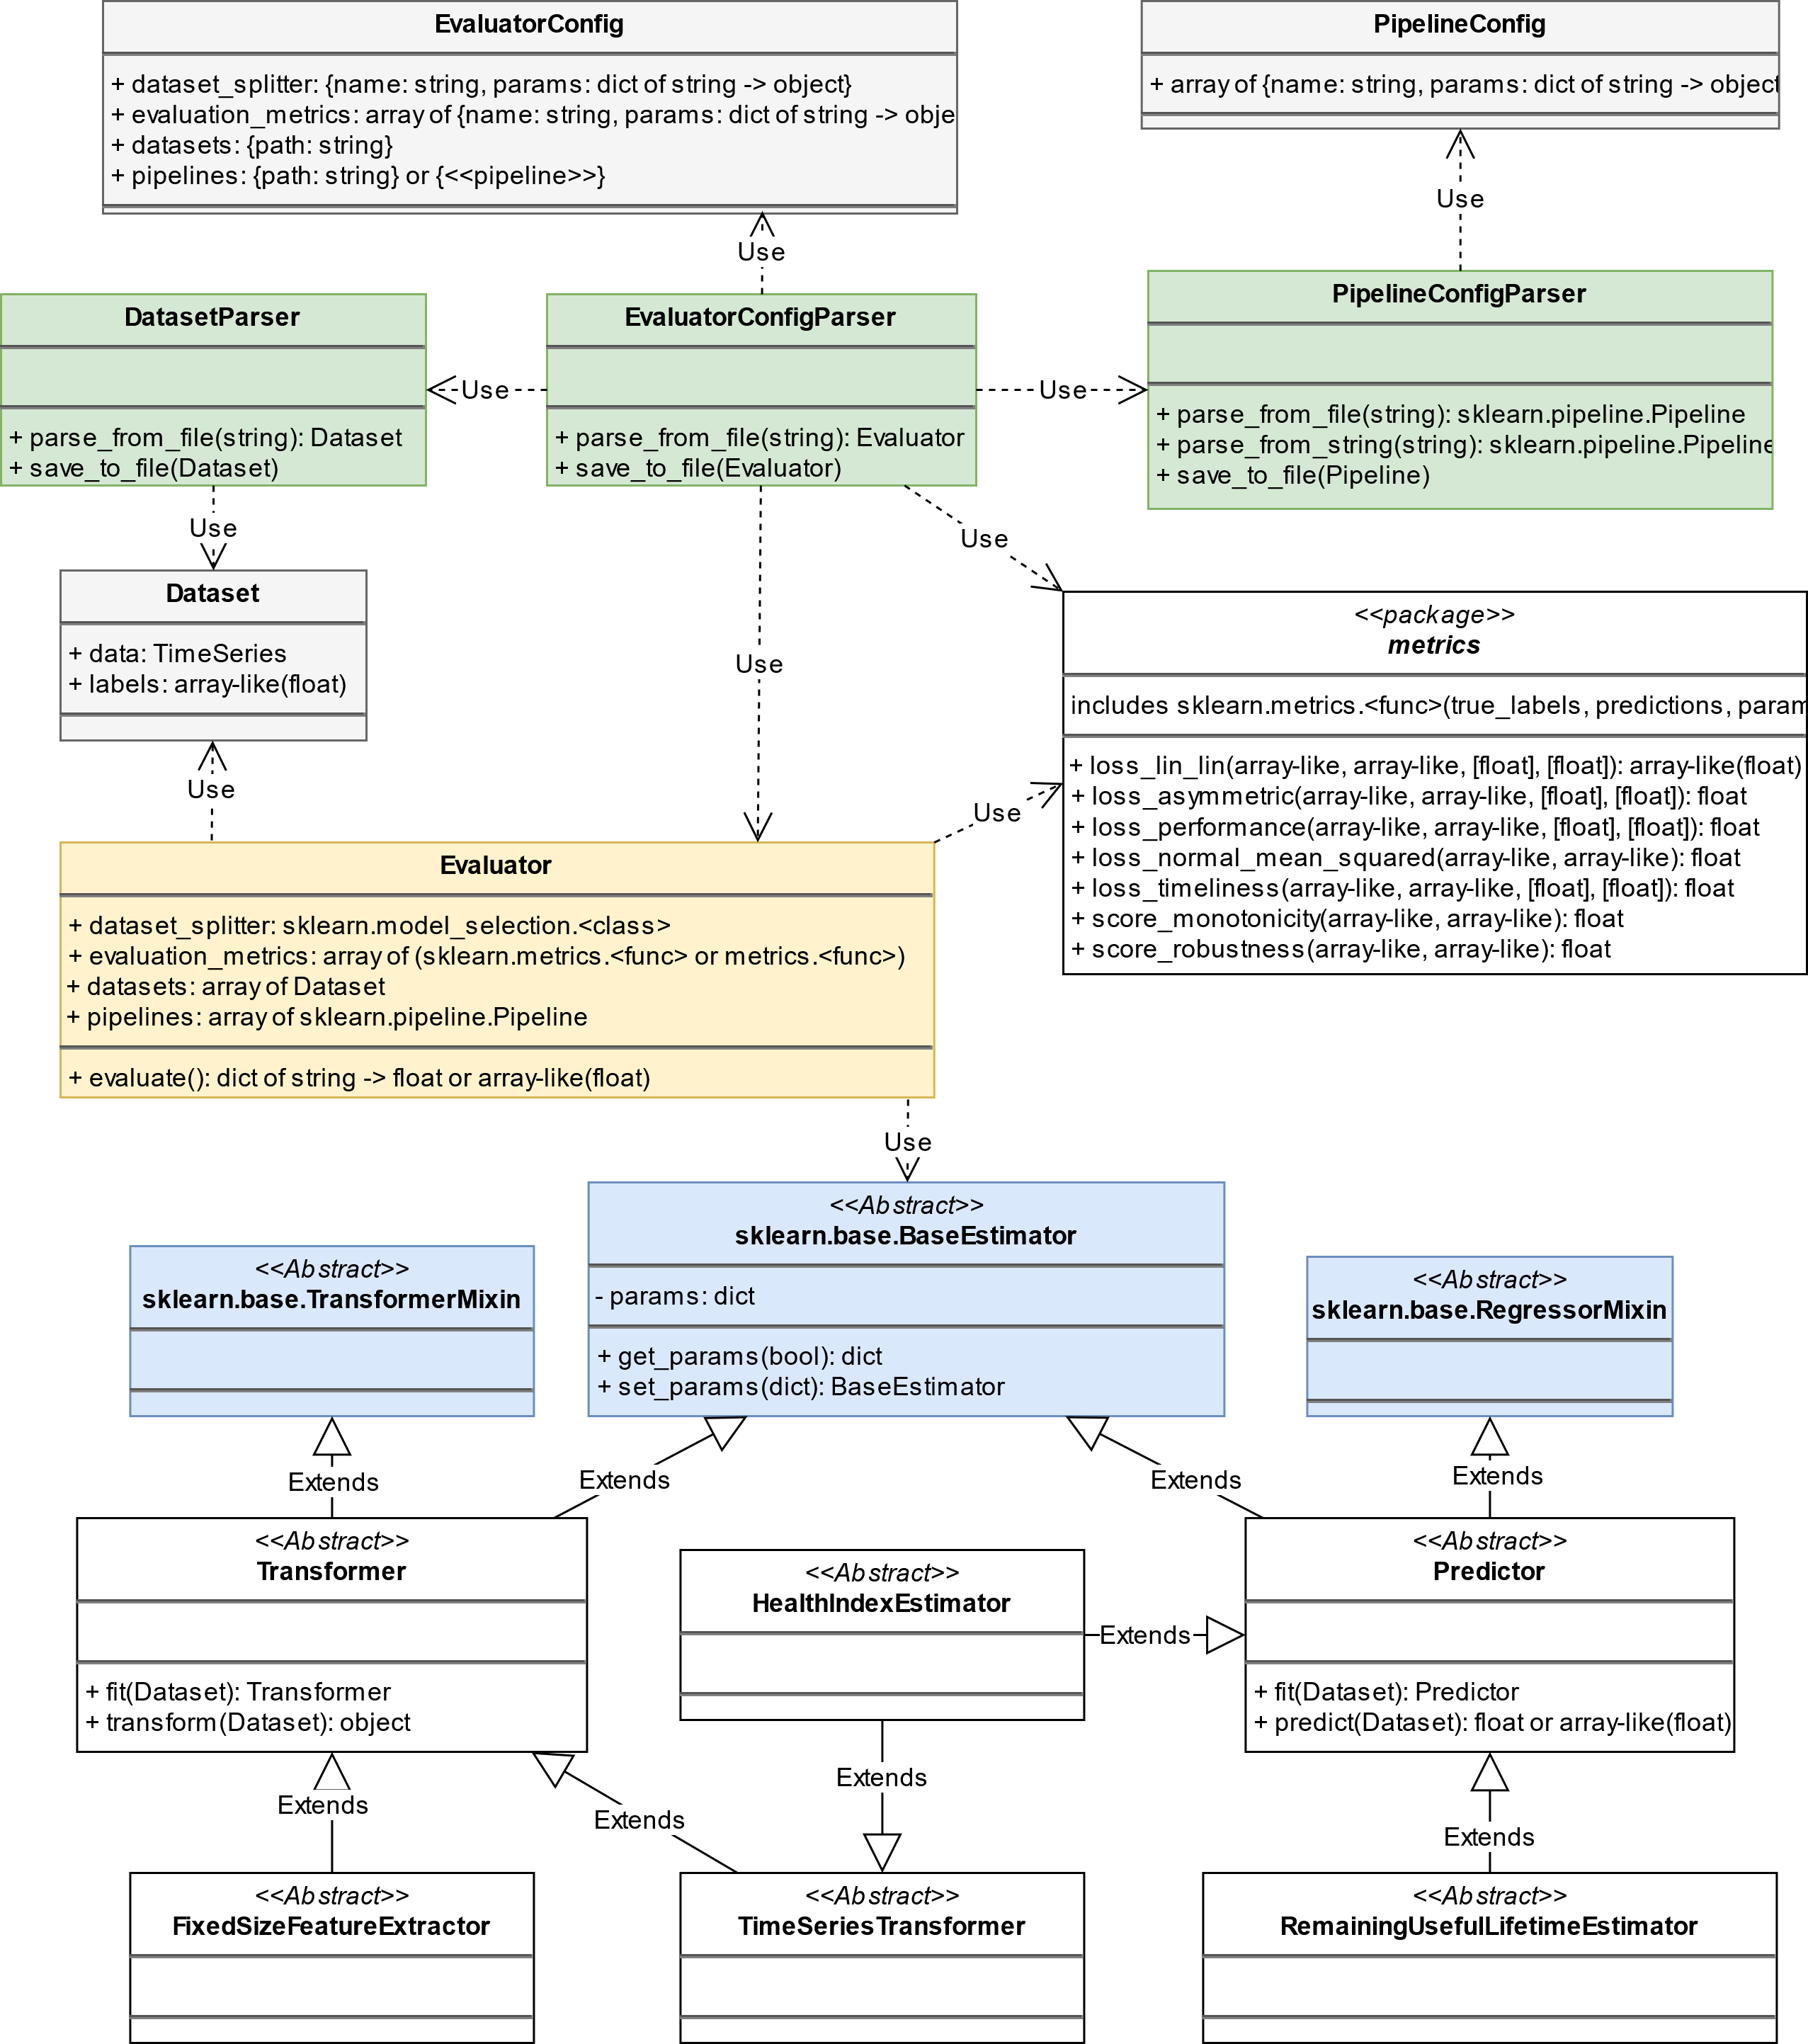
\includegraphics[width=\textwidth]{gfx/general_class_diagram}
    \caption{Class diagram showing general classes and interrelations}
    \label{fig:interfaces-general_class_diagram}
\end{figure}

\subsection*{Sequence diagram}
\vspace*{-10mm}\hfill{\fontfamily{phv}\normalsize\emph{Paul Fährmann}}
\\
The first general sequence diagram shown in Figure~\ref{fig:interfaces-general_sequence_diagram} describes the use case for loading evaluating one pipeline on one data set using the \textit{Evaluator} class. We first load the dataset via the \textit{DatasetParser}, then create a Pipeline with the \textit{make\_pipeline} call. We also create a \textit{splitter} object which is used to split the data into training and test subsets. When creating the \textit{Evaluator}, we give the dataset, the pipeline, the splitter and the metric-functions to the constructor. In the \textit{evaluate} function call of the \textit{Evaluator} object we have four nested loops.
\begin{enumerate}
    \item The first one loops over the data sets and splits them into a \textit{train\_dataset} and a \textit{test\_dataset}.
    \item In the second one we loop over the pipelines, which includes fitting the pipeline on the training set and predicting via the testing set.
    \item The third loop goes over the created splits of the data set in which the fit and the transform functions of the pipeline are called.
    \item The fourth one loops over the metrics as we now evaluate the loss or the score of the prediction for that pipeline. Here we get the \textit{evaluation\_result} back which is then concatenated or combined into the end result.
\end{enumerate}

\begin{figure}[ht]
    \centering
    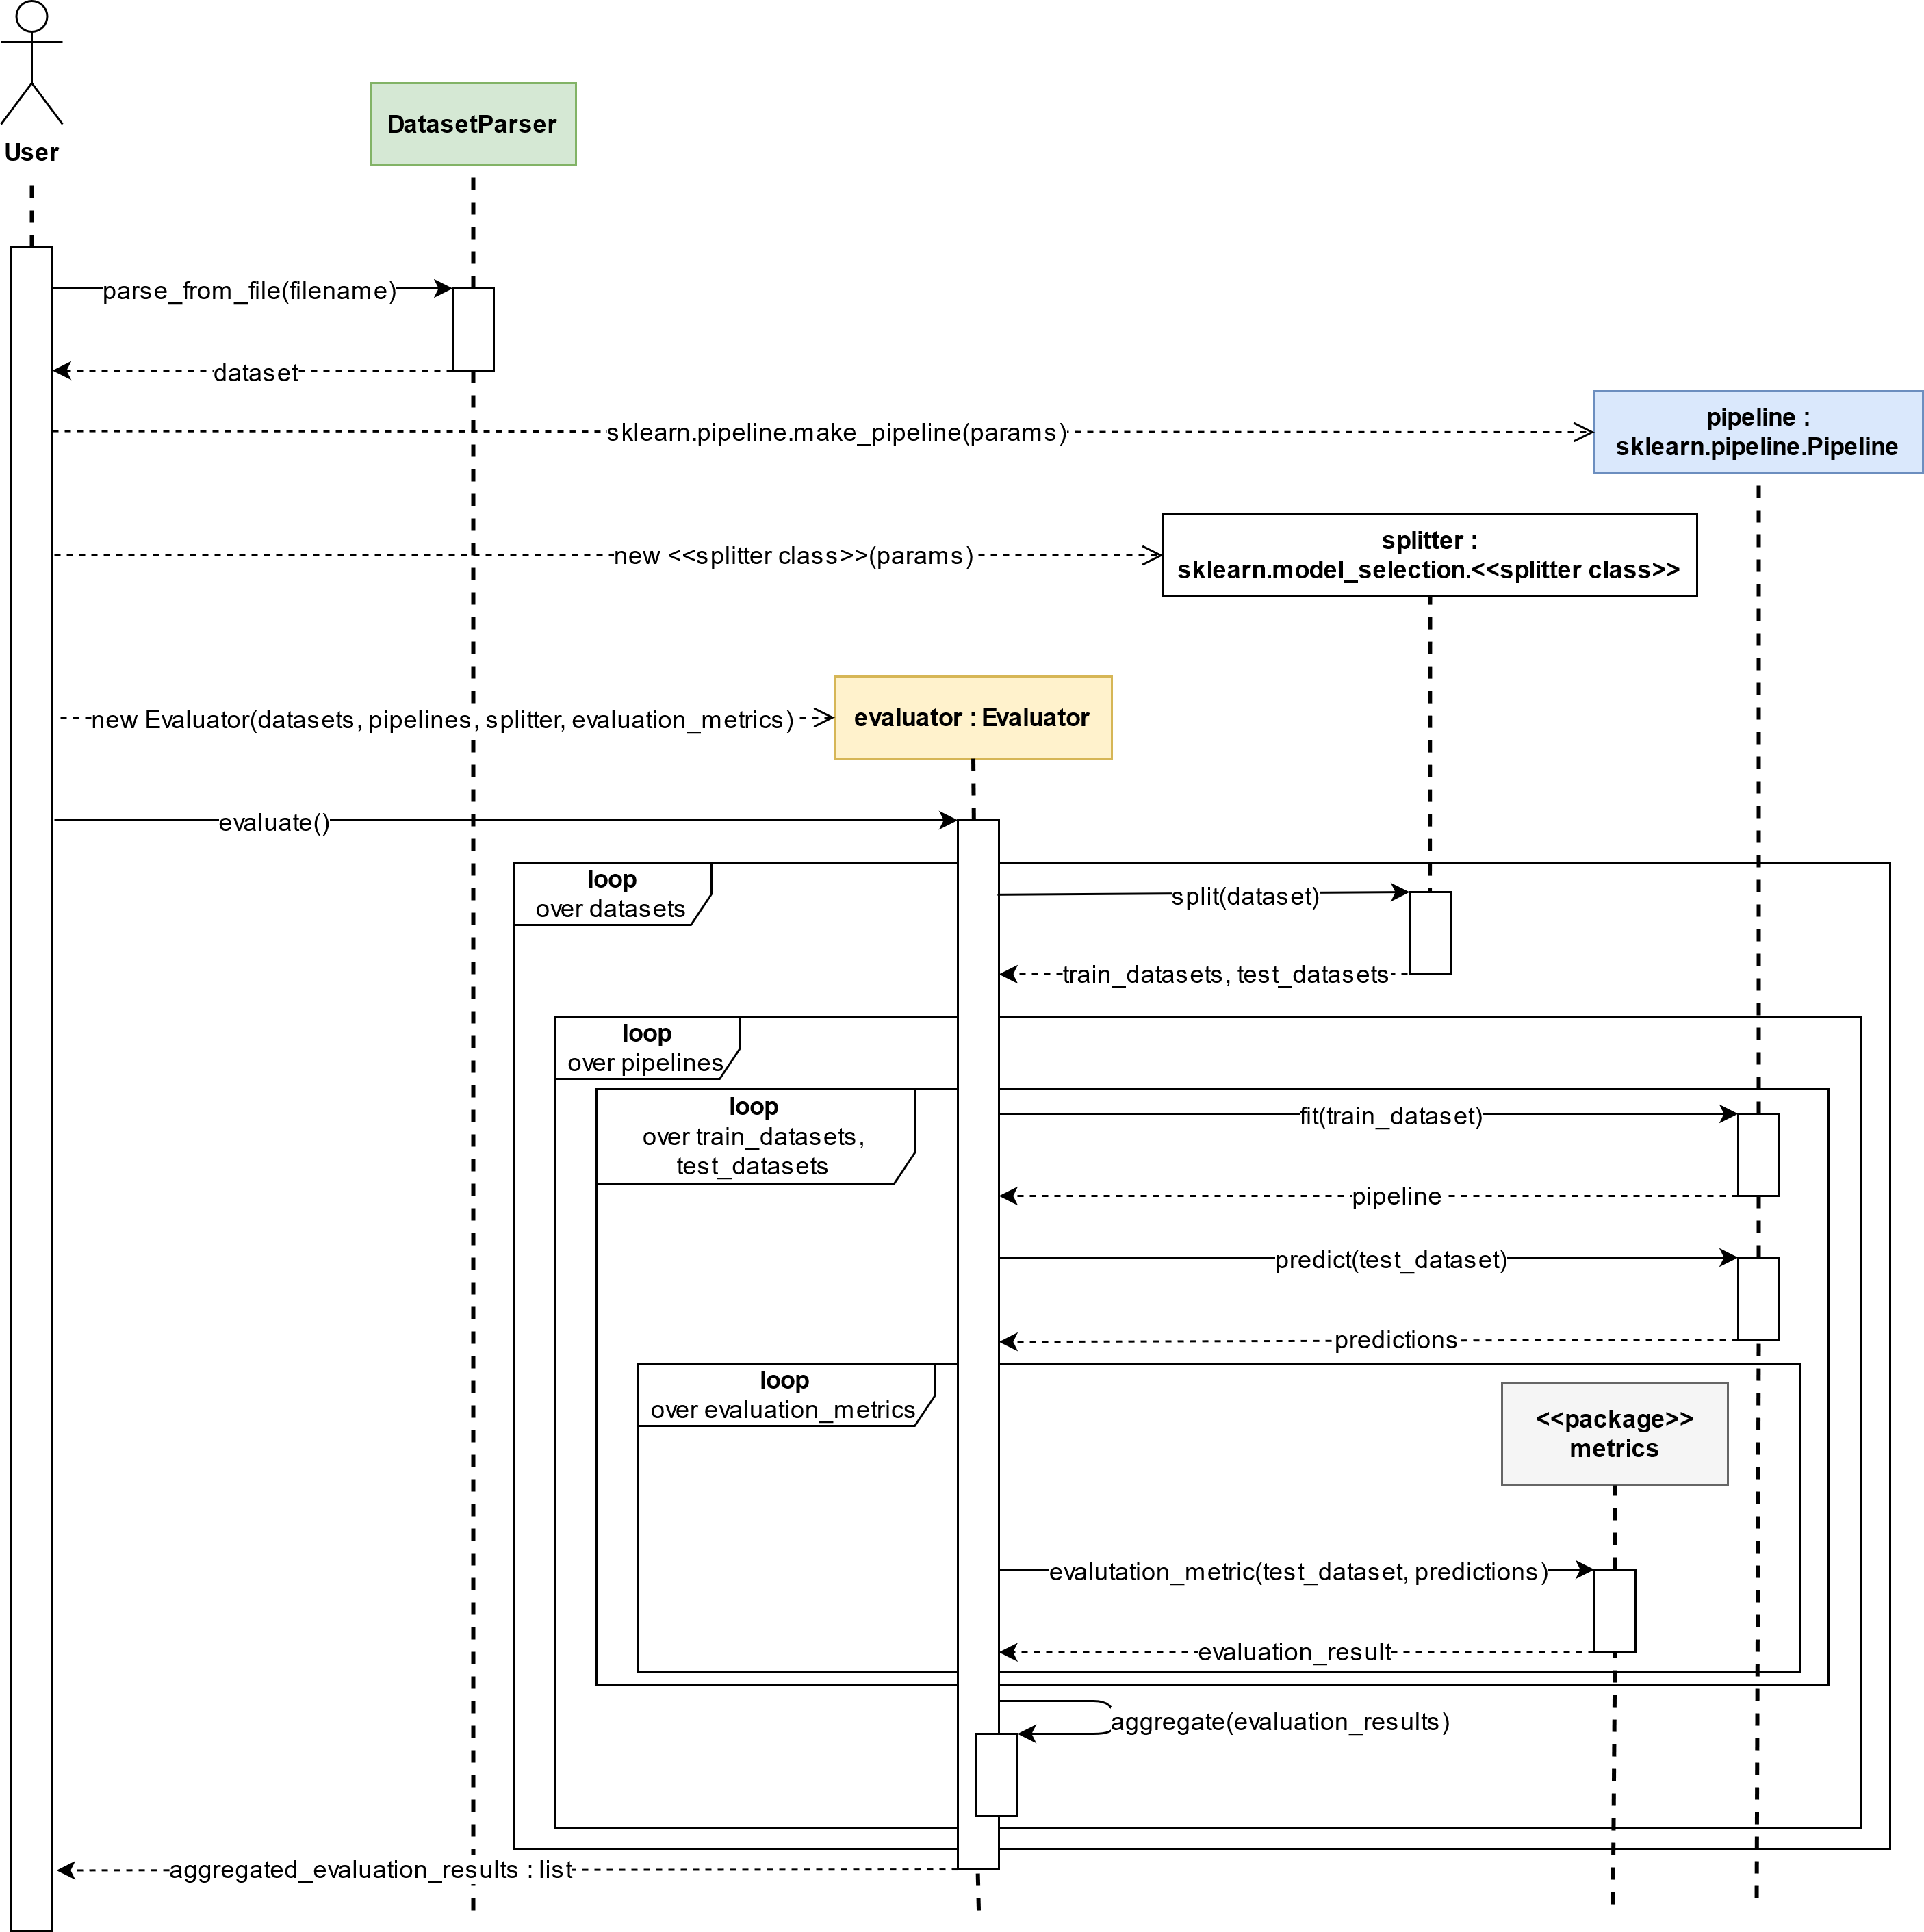
\includegraphics[width=\textwidth]{gfx/general_sequence_diagram}
    \caption{Sequence diagram showing the general flow of actions when starting from scratch.}
    \label{fig:interfaces-general_sequence_diagram}
\end{figure}

The second general sequence diagrams shown in Figure~\ref{fig:interfaces-general_sequence_diagram_with_config} describes the use case of loading an \textit{Evaluator} from a configuration file via the \textit{EvaluatorConfigParser}.
In the parsing of the configuration file the \textit{EvaluatorConfigParser} has three loops, which are however not nested.
\begin{itemize}
    \item The first loop goes over the \textit{dataset\_paths} which uses the \textit{DatasetParser} to load the datasets.
    \item The second loop goes over the \textit{pipeline\_paths} which uses the \textit{PipelineConfigParser} to load the pipeline configuration and then uses its internal pipeline parser function \textit{parse\_from\_string} to create the pipelines.
    \item The third loop goes over the pipeline configuration strings that are put into the evaluator configuration directly. These are parsed to create the pipelines.
\end{itemize}
After these loops the \textit{splitter} is created and the \textit{Evaluator} object is constructed with the now loaded datasets, pipelines, splitter and metrics, which are loaded directly.
\begin{figure}[ht]
    \centering
    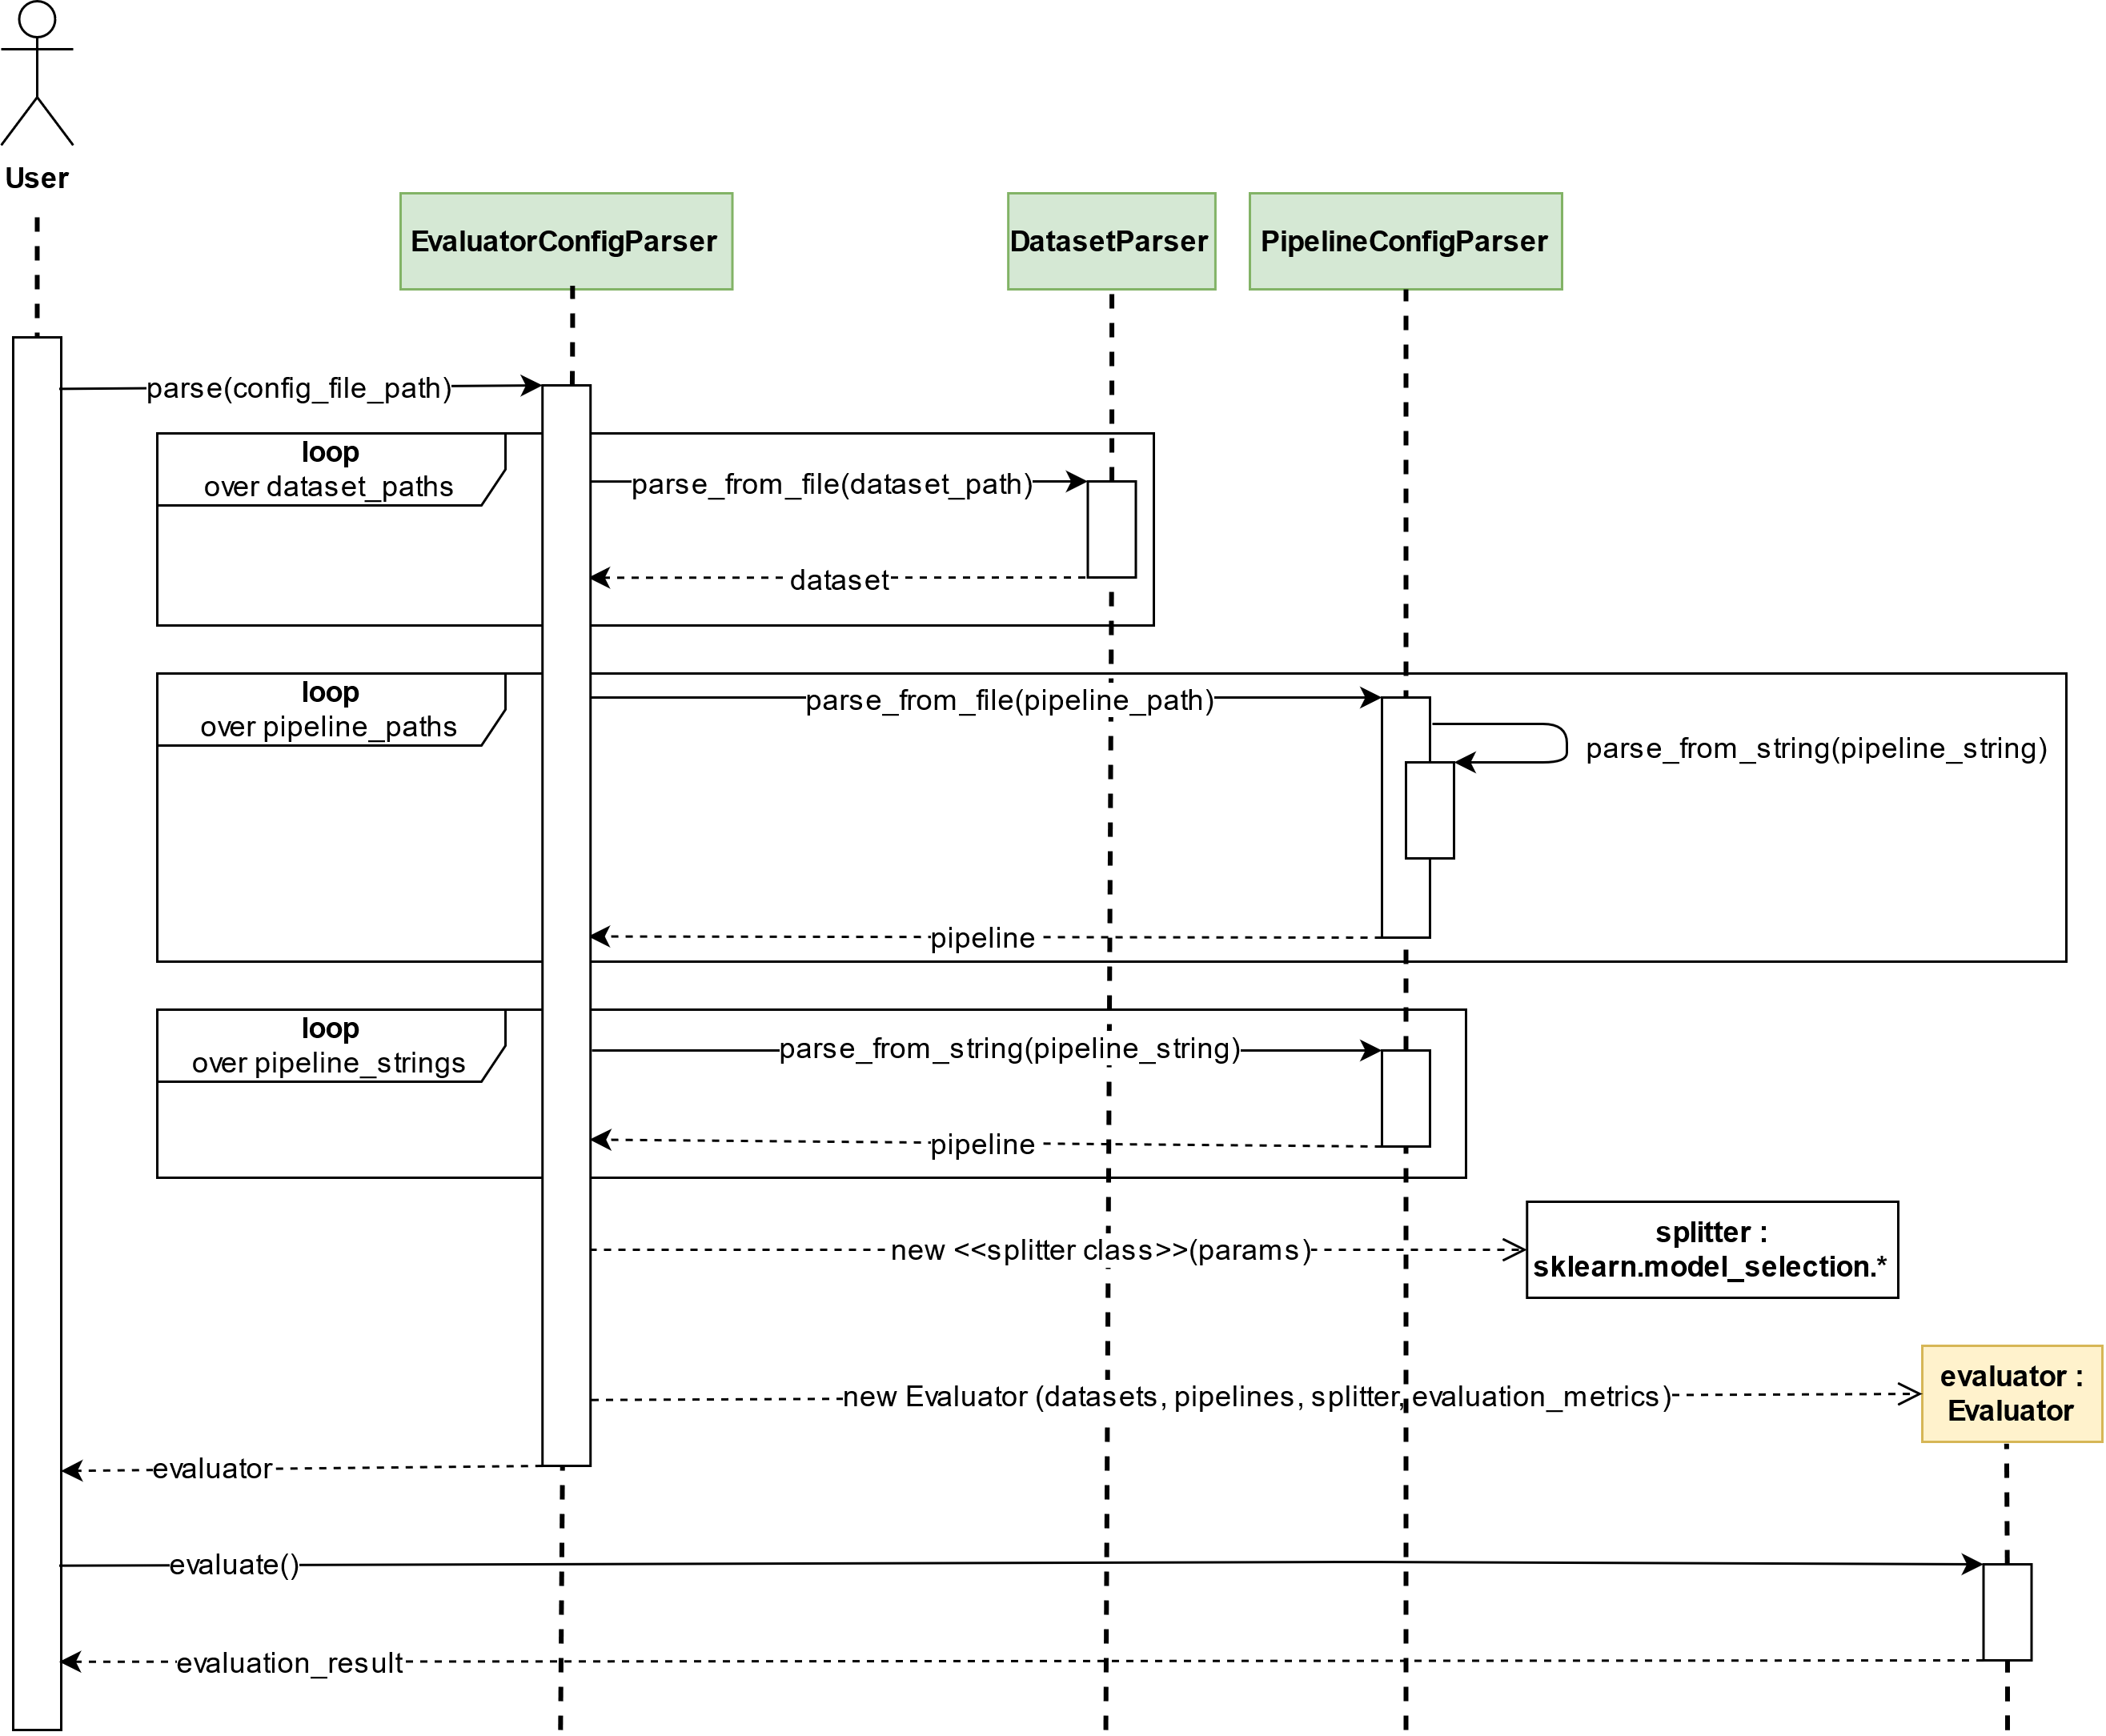
\includegraphics[width=\textwidth]{gfx/general_sequence _diagram_config}
    \caption{Sequence diagram showing the general flow of actions when starting with some predefined approach and evaluation.}
    \label{fig:interfaces-general_sequence_diagram_with_config}
\end{figure}

\section{Time Series Feature Extraction}
\vspace*{-5mm}\hfill{\fontfamily{phv}\normalsize\emph{Paul Fährmann, Sanjay Gupta}}
\\
In this chapter we show the class and sequence diagrams regarding to the classes in the feature extraction and preprocessing steps of our library.
\subsection*{Class diagram}
\vspace*{-5mm}\hfill{\fontfamily{phv}\normalsize\emph{Paul Fährmann, Sanjay Gupta}}
\\
The Figures \ref{fig:interfaces-tfe-fixedsize} and \ref{fig:interfaces-tfe-transformer} demonstrate the class diagram of time series feature extraction. Every class that inherits from the \textit{FixedSizeFeatureExtractor} abstract class transforms a time series into a fixed length vector of real valued features. These are \textit{RNNAutoencoder} which represents a time series into a fixed dimension using neuronal networks, \textit{TSFreshWrapper} which extracts basic statistical features, \textit{PytsTransformWrapper} which includes several methods of extracting feature vectors and \textit{MovingWeightedAverage} which calculates one moving weighted value of a time series.

\begin{figure}[ht]
    \centering
    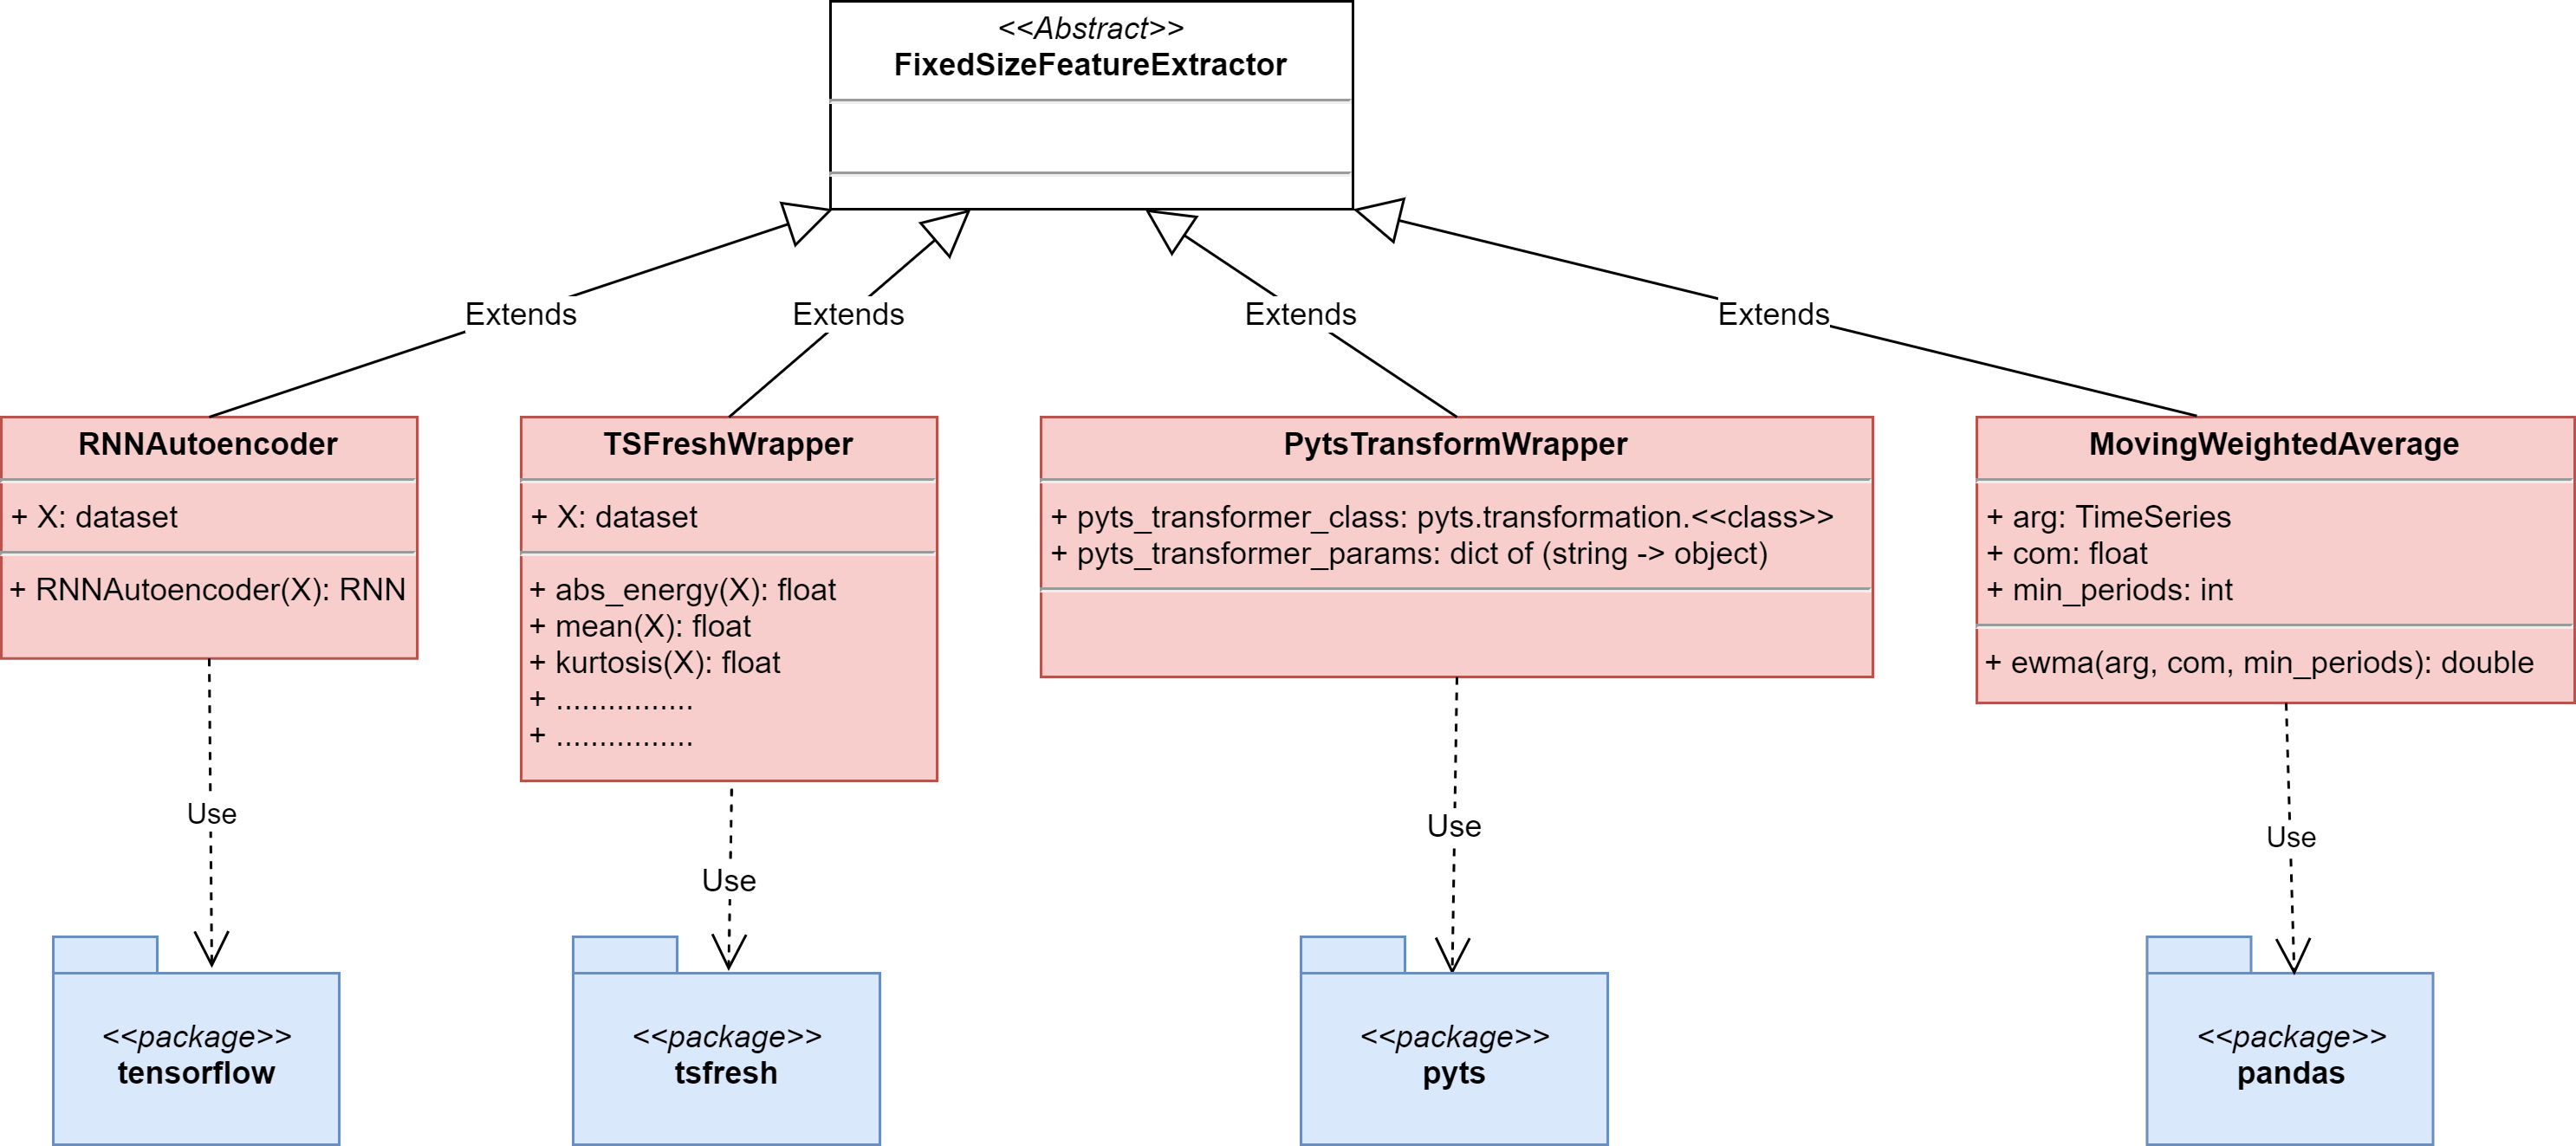
\includegraphics[width=\textwidth]{gfx/Interfaces-TFE-FixedSize.png}
    \caption{Class diagram of Fixed size feature extractor.}
    \label{fig:interfaces-tfe-fixedsize}
\end{figure}
Every class that inherits from the \textit{TimeSeriesTransformer} abstract class transforms a time series into another time series. These are the \textit{TimeSeriesImputer} which imputes timestamp-value pairs, \textit{EMDSignalWrapper} and \textit{PywtWrapper} which extract and filter the time series and the \textit{WindowingApproach} which cuts the time series into same size chunks.
\begin{figure}[ht]
    \centering
    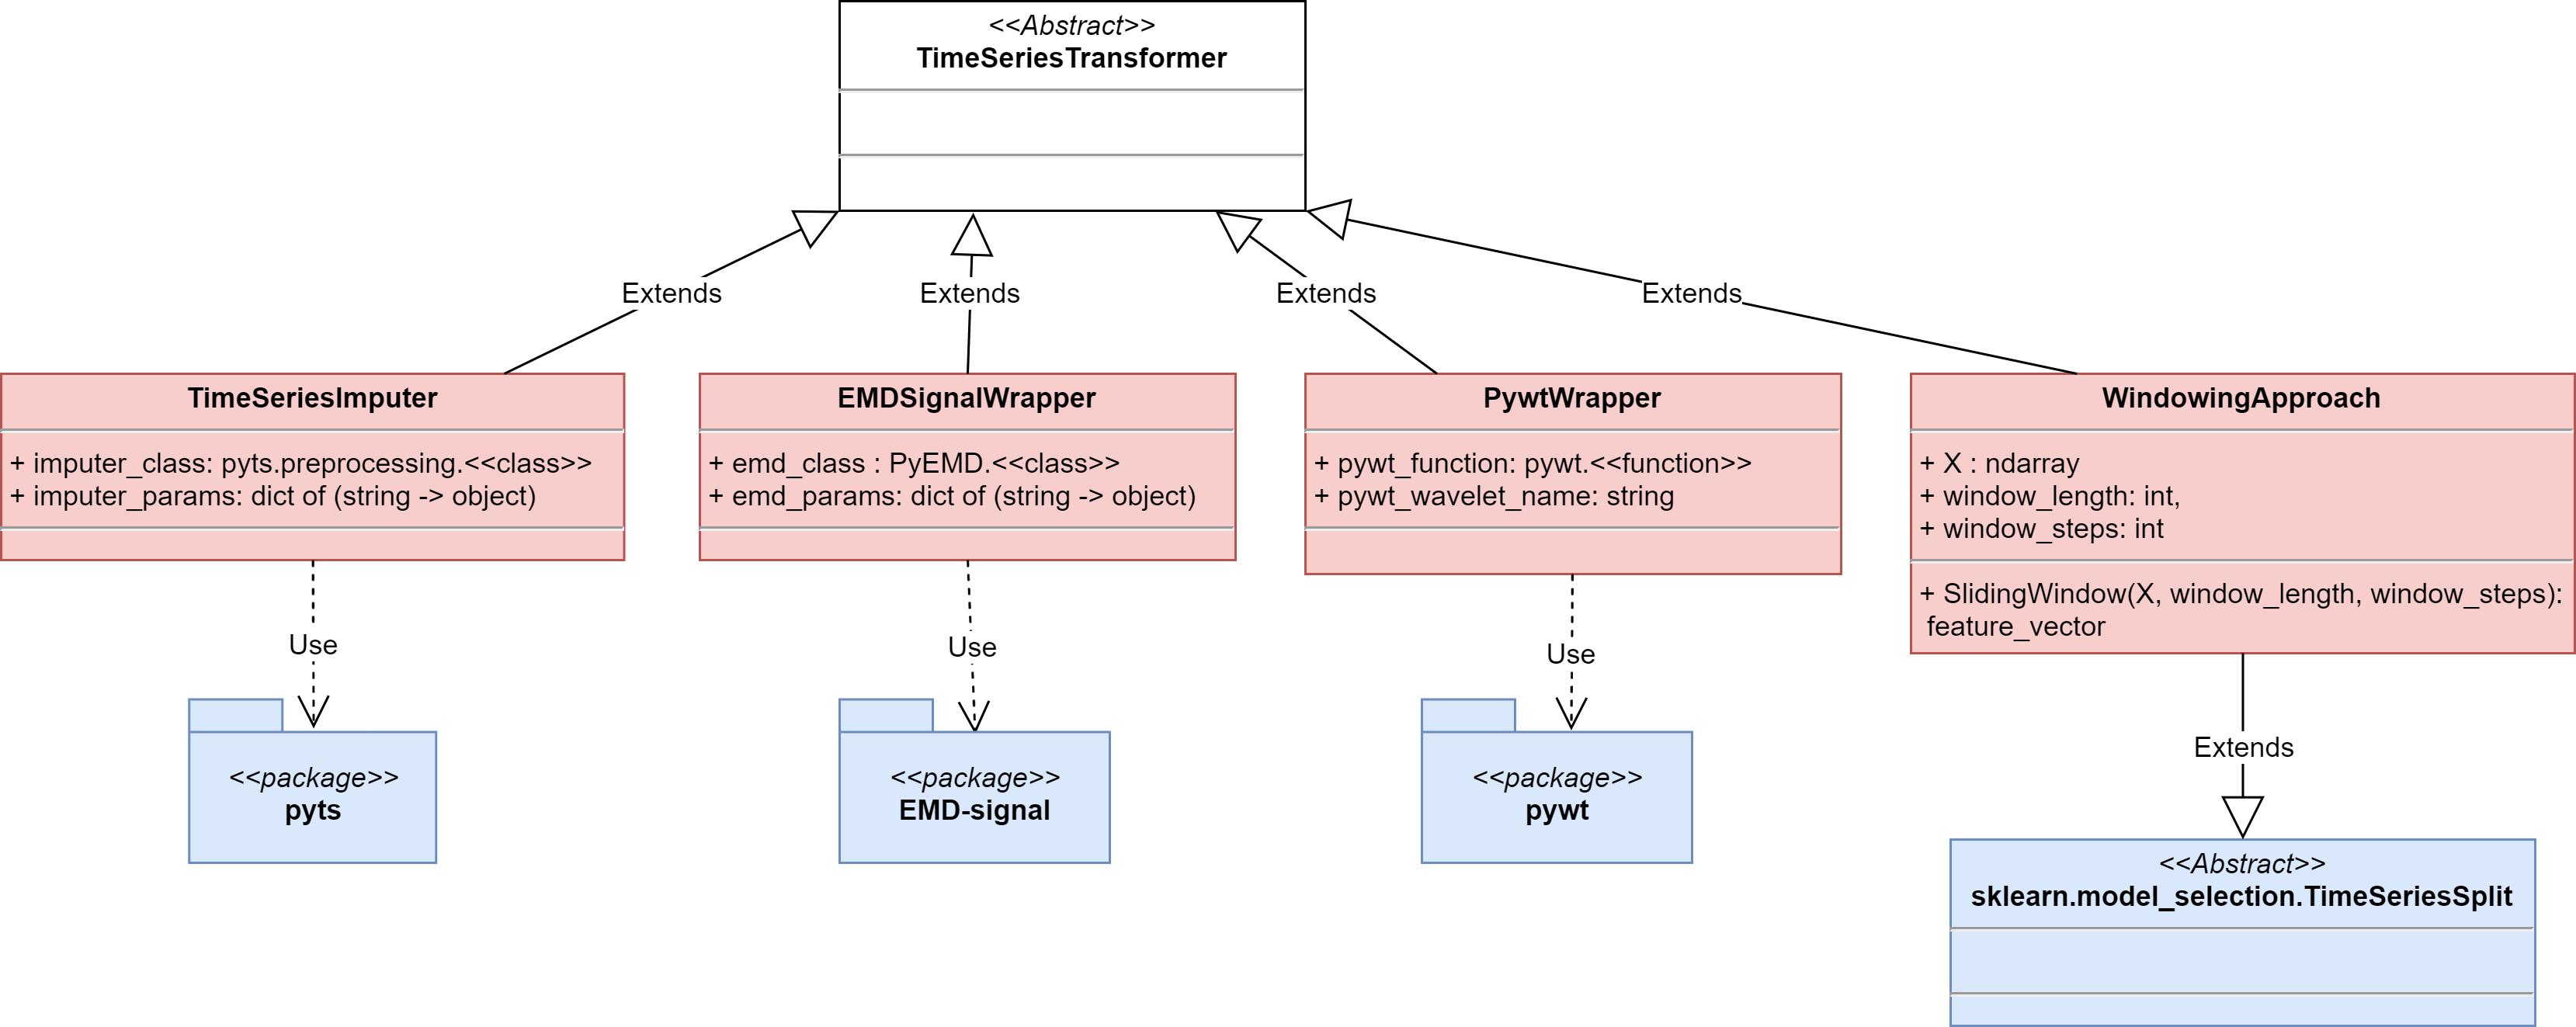
\includegraphics[width=\textwidth]{gfx/Interfaces-TFE-Transformer.png}
    \caption{Class diagram of Time Series Transformer.}
    \label{fig:interfaces-tfe-transformer}
\end{figure}
The \textit{UniToMultivariateWrapper} class applies the specified transformer on all time series. The transformers class can either be a \textit{TimeSeriesTransformer} or a \textit{FixedSizeFeatureExtractor}.
\begin{figure}[ht]
    \centering
    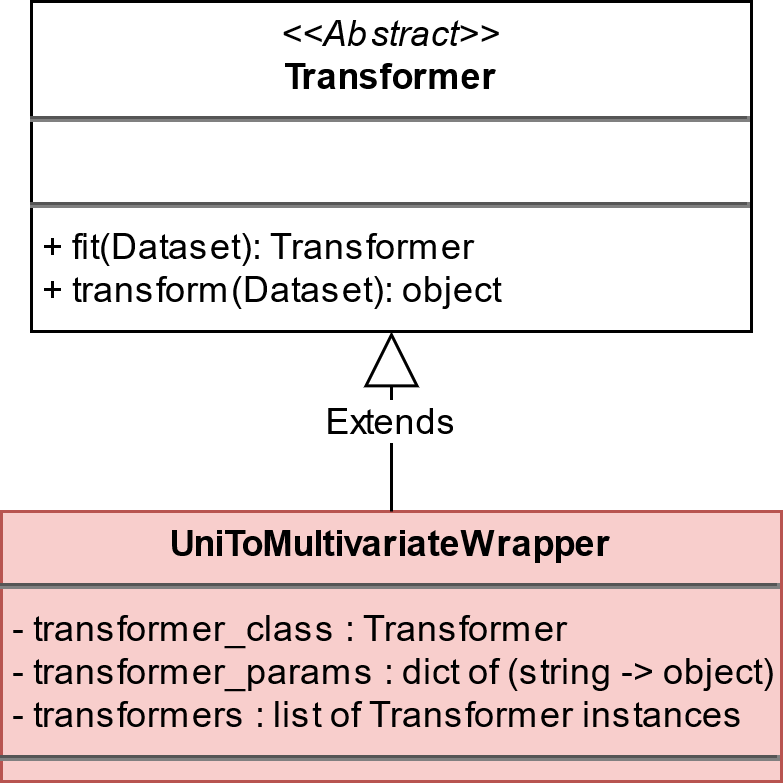
\includegraphics[width=.4\textwidth]{gfx/uni_to_multivariate_wrapper_class}
    \caption{Class diagram showing general classes and interrelations}
    \label{fig:interfaces-tfe-unitomulti}
\end{figure}
\newpage
\subsection*{Sequence diagram}
We are explaining the fit and transform use cases for the different time series feature extraction and preprocessing classes.
\subsubsection*{UniToMultivariateWrapper}
\vspace*{-10mm}\hfill{\fontfamily{phv}\normalsize\emph{Paul Fährmann}}
\\
The \textit{UniToMultivariateWrapper} applies a transformation to each sensor data (univariate time series) of the dataset and aggregates the transformed data at the end. We specify the used \textit{transformer\_class} with the \textit{transformer\_params} in the constructor.
\begin{figure}[ht]
    \centering
    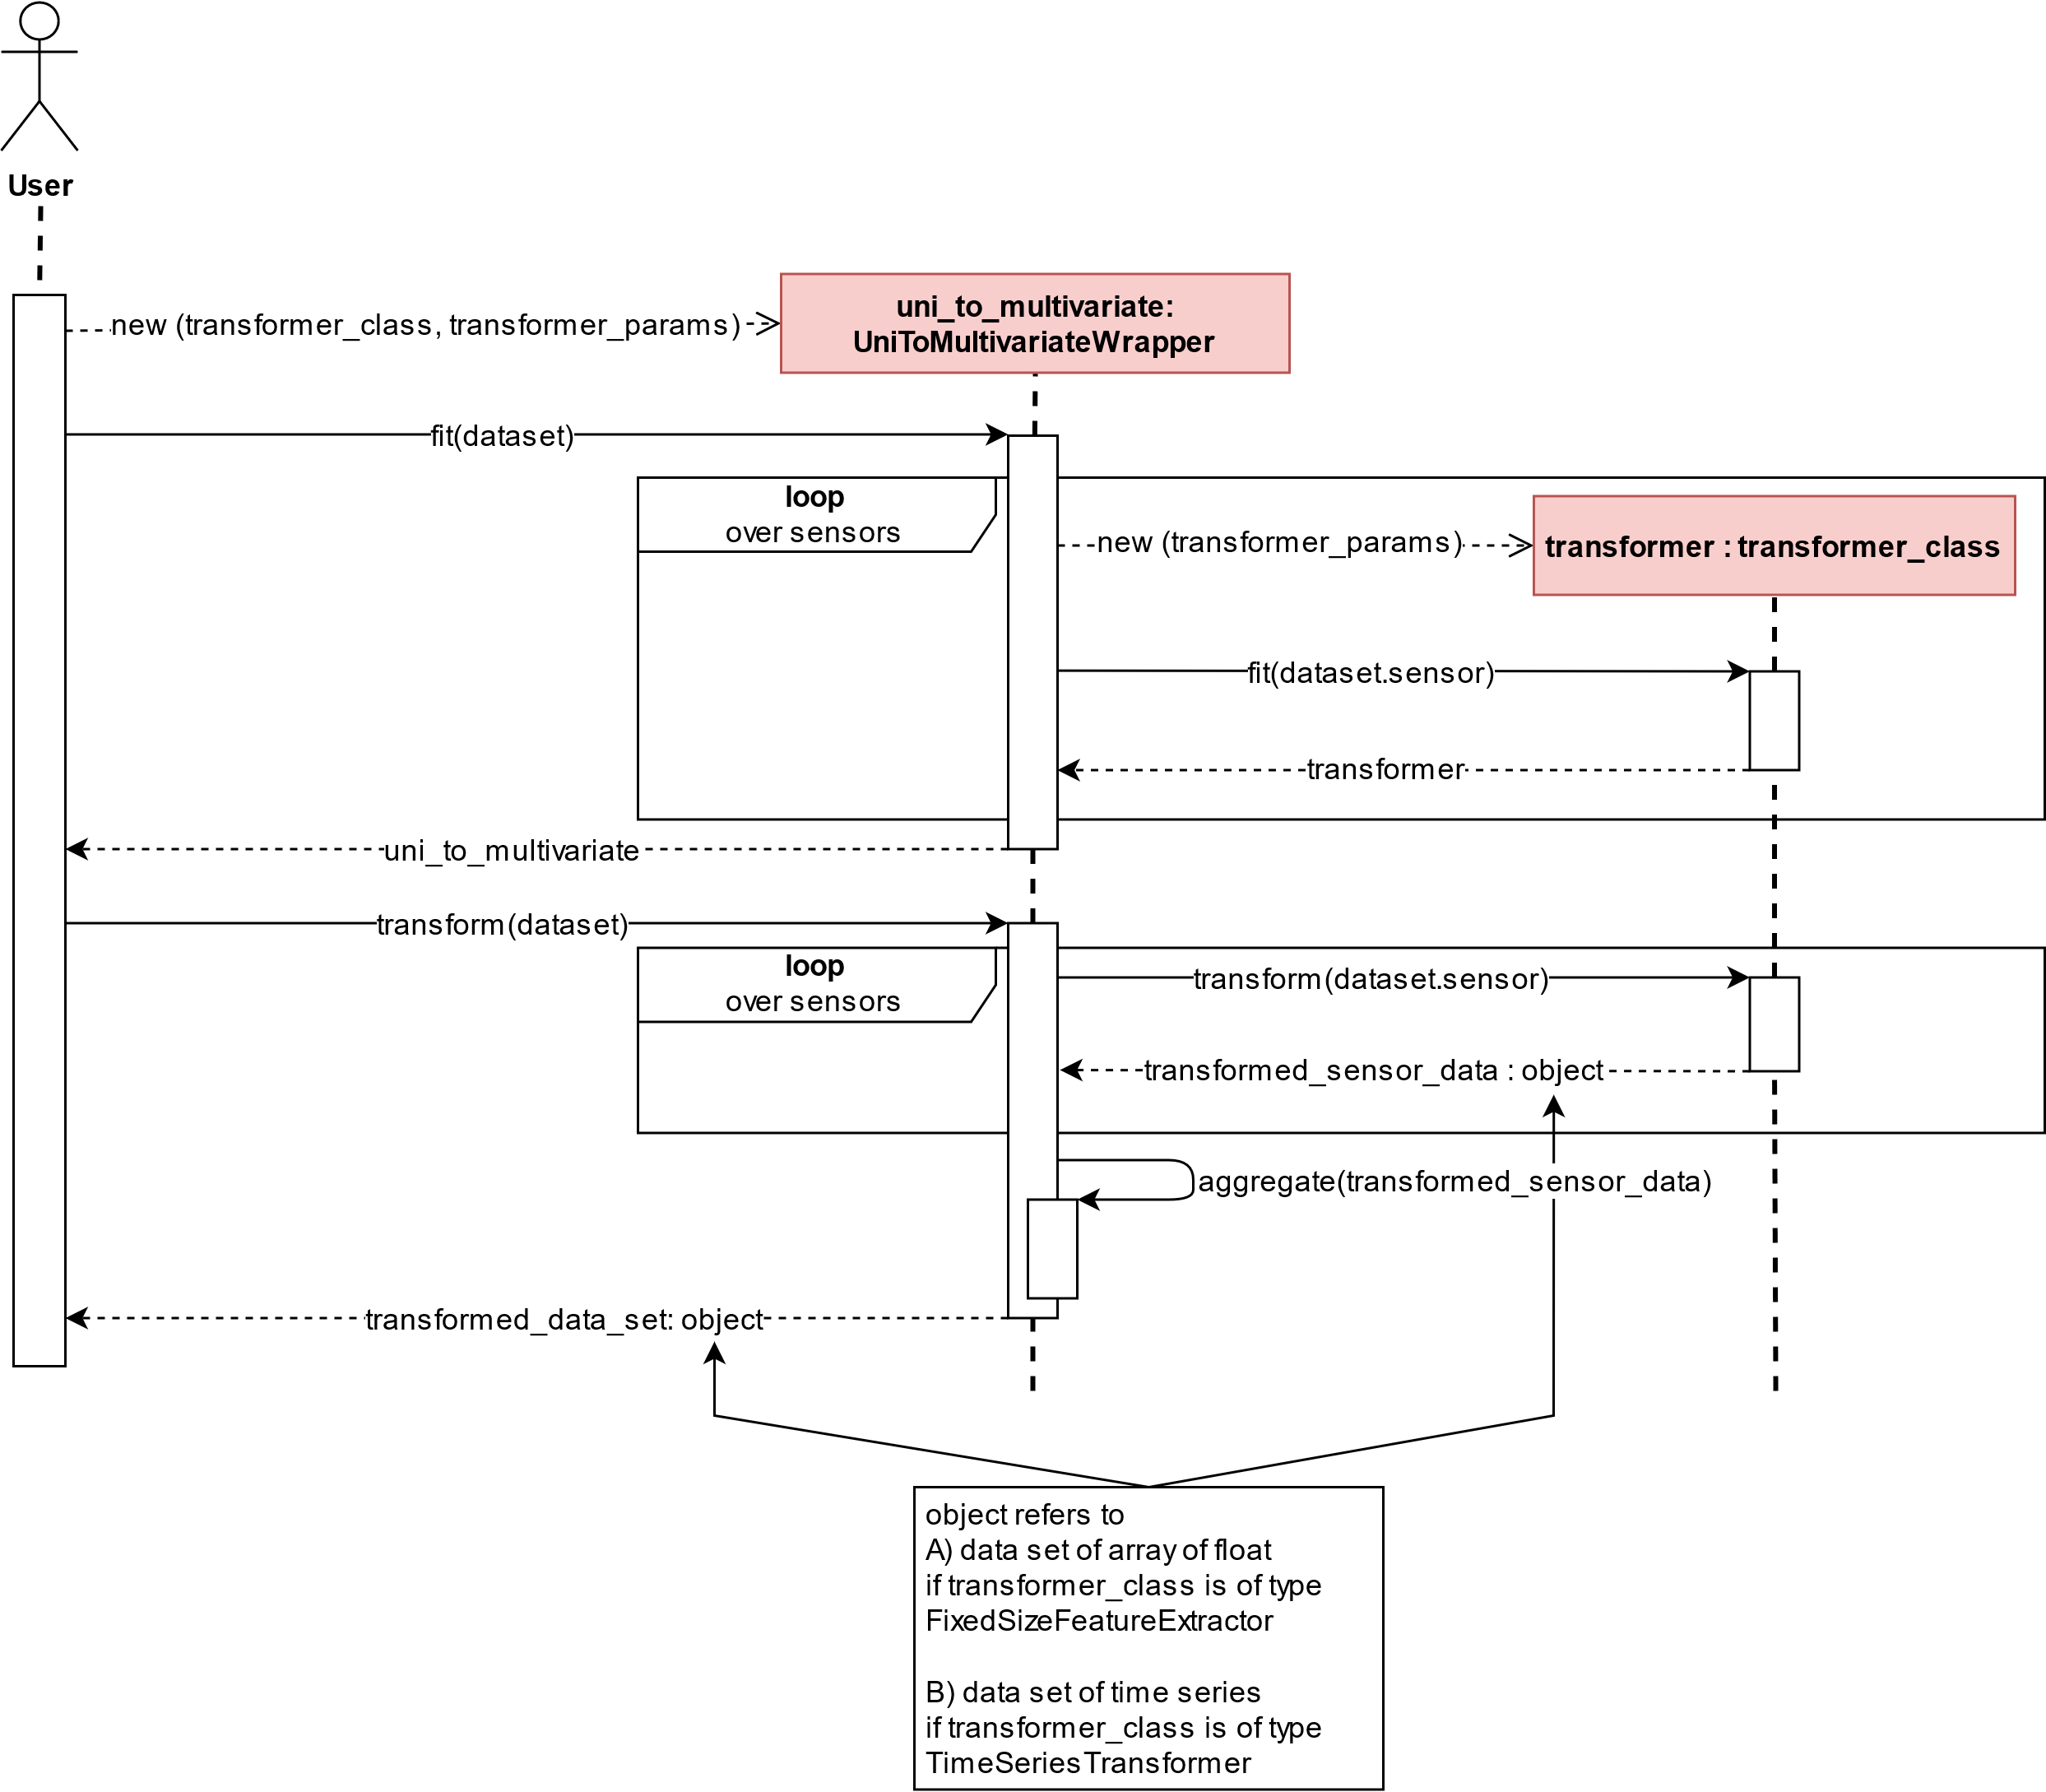
\includegraphics[width=\textwidth]{gfx/uni_to_multi_sequence}
    \caption{Sequence Diagram of the UniToMultivariateWrapper class for fit and transform use-case.}
    \label{fig:uni-to-multi-seq}
\end{figure}
In Figure~\ref{fig:uni-to-multi-seq}, we show the use case for the fit and the transform function call. In the fit call we loop over the sensors and create a transformer object for each sensor respectively and also call the fit function on that transformer. These transformers are saved in a list \textit{transformers} as member parameters. In the \textit{transform} function call we again loop over the sensors and call the transform on the fitted transformer for that sensor from our list of transformers. After transforming these sensors we aggregate the result. If our specified transformer class is of type \textit{TimeSeriesTransformer} we transform each individual sensor time series into the new form for an instance of the dataset. If our specified transformer class is of type \textit{FixedSizeFeatureExtractor} we concatenate the resulting fixed size vectors of the sensors to one vector for an instance of the dataset.
\subsubsection*{PywtWrapper}
\vspace*{-10mm}\hfill{\fontfamily{phv}\normalsize\emph{Paul Fährmann}}
\\
The \textit{PywtWrapper} is a wrapper for the PyWavelet library \textit{pywt}\footnote{\href{https://pywavelets.readthedocs.io/en/latest/}{https://pywavelets.readthedocs.io/en/latest/}}. The \textit{pywt} package contains several wavelet transformation functions that scan over the time and frequency domain of the data. We specify the used transformation function \textit{pywt\_function} and the wavelet function name \textit{pywt\_wavelet\_name} in the constructor of the \textit{PywtWrapper}. In Figure~\ref{fig:tfe-pywt-seq}, we show the use case for the fit and the transform function call. In the fit call nothing happens, as nothing from the dataset needs to be known before. In the transform function call, the specified wavelet transformation function is called with the dataset and the specified wavelet function. We get back the wavelet-coefficients.
\begin{figure}[ht]
    \centering
    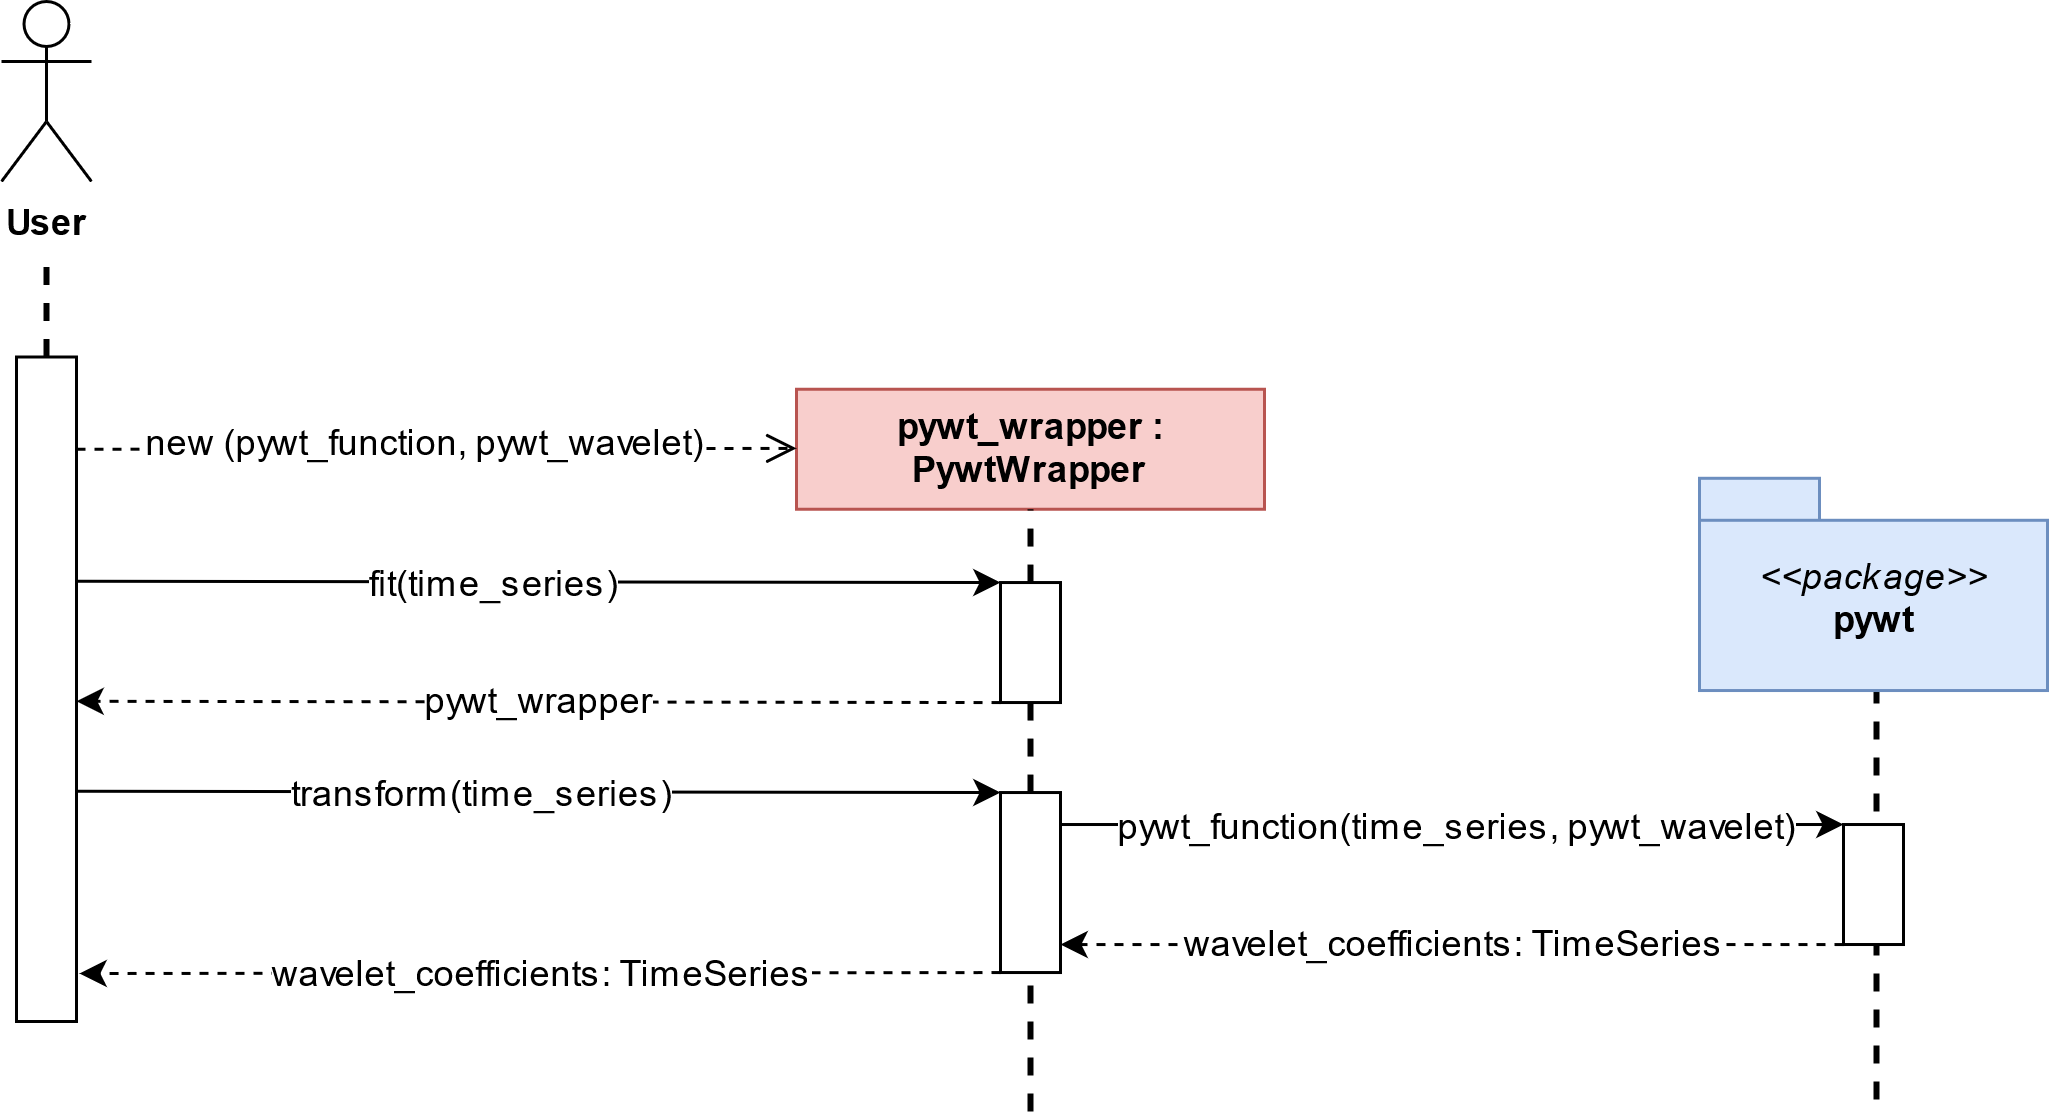
\includegraphics[width=\textwidth]{gfx/pywt_sequence}
    \caption{Sequence Diagram of the PywtWrapper class for fit and transform use-case.}
    \label{fig:tfe-pywt-seq}
\end{figure}
\newpage
\subsubsection*{EMDSignalWrapper}
\vspace*{-10mm}\hfill{\fontfamily{phv}\normalsize\emph{Paul Fährmann}}
\\
The \textit{EMDSignalWrapper} is a wrapper for the EMD-Signal library \textit{PyEMD}\footnote{\href{https://pypi.org/project/EMD-signal/}{https://pypi.org/project/EMD-signal/}}. This library contains several EMD classes. We specify the used class of that library and the constructor parameters in the \textit{EMDSignalWrapper} constructor and create the \textit{emd\_class} object with the specified params. In Figure~\ref{fig:tfe-emd-signal-seq}, we show the use case for the fit and the transform function call. The fit function call does nothing, but in the transform call, the emd object is used to calculate the imf components for the time series in given dataset.
\begin{figure}[ht]
    \centering
    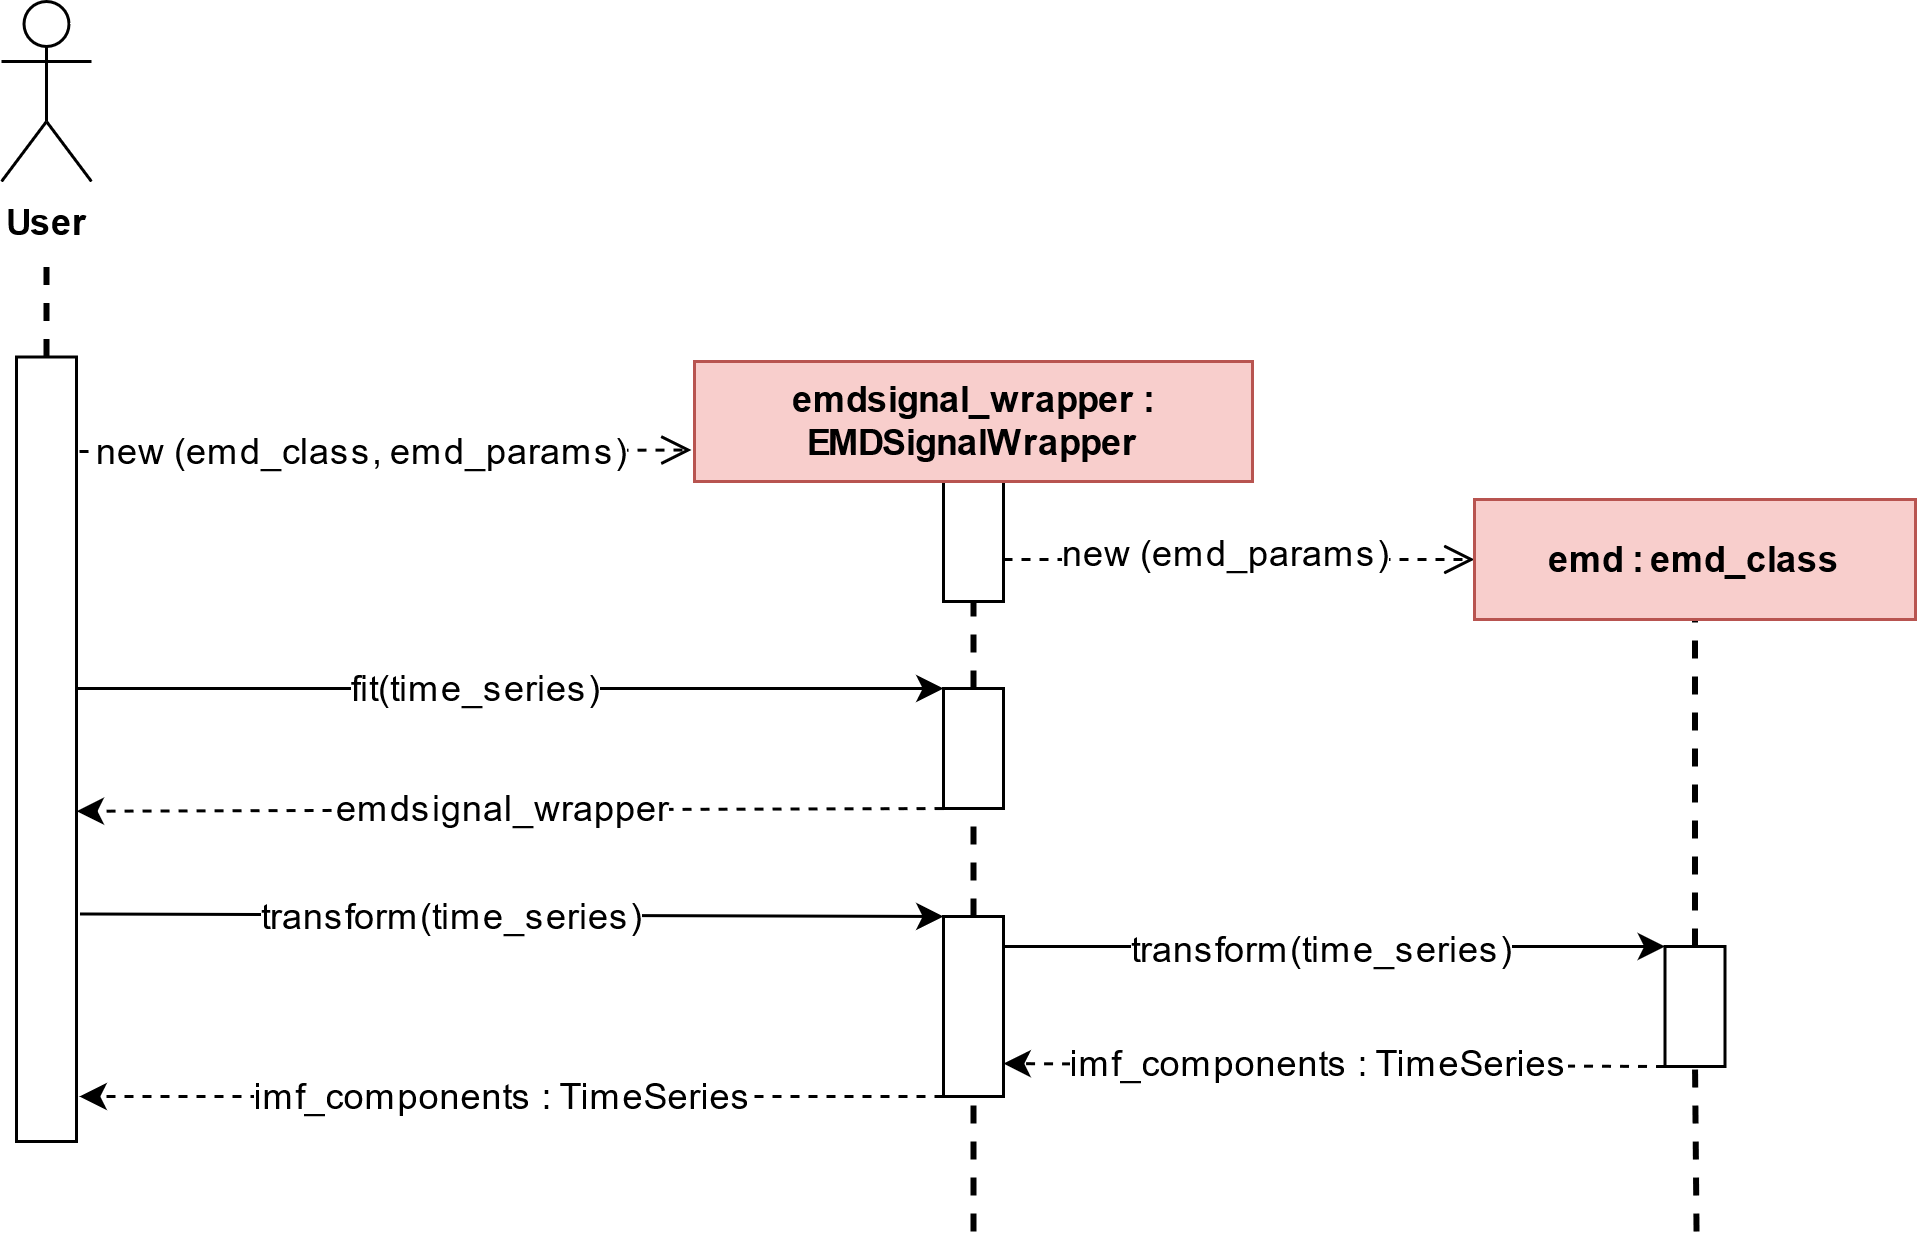
\includegraphics[width=\textwidth]{gfx/emdsignal_sequence}
    \caption{Sequence Diagram of the EMDSignalWrapper class for fit and transform use-case.}
    \label{fig:tfe-emd-signal-seq}
\end{figure}
\subsubsection*{TimeSeriesImputer}
\vspace*{-10mm}\hfill{\fontfamily{phv}\normalsize\emph{Paul Fährmann}}
\\
The \textit{TimeSeriesImputer} is a wrapper for the \textit{pyts.preprocessing}\footnote{\href{https://pypi.org/project/pyts/}{https://pypi.org/project/pyts/}} imputer classes that can be extended in the implementation phase to a more general imputer for time series, hence the name. We specify the class and the constructor params of the imputer class in the \textit{PytsImputeWrapper} constructor and create the \textit{pyts\_imputer\_class} object with the specified params. In Figure~\ref{fig:tfe-pyts-impute-seq}, we show the use case for the fit and the transform function call. In the \textit{fit} call we call the fit function of that imputer and get back the imputer. In the \textit{transform} call we just call the transform function of the imputer class object.
\begin{figure}[ht]
    \centering
    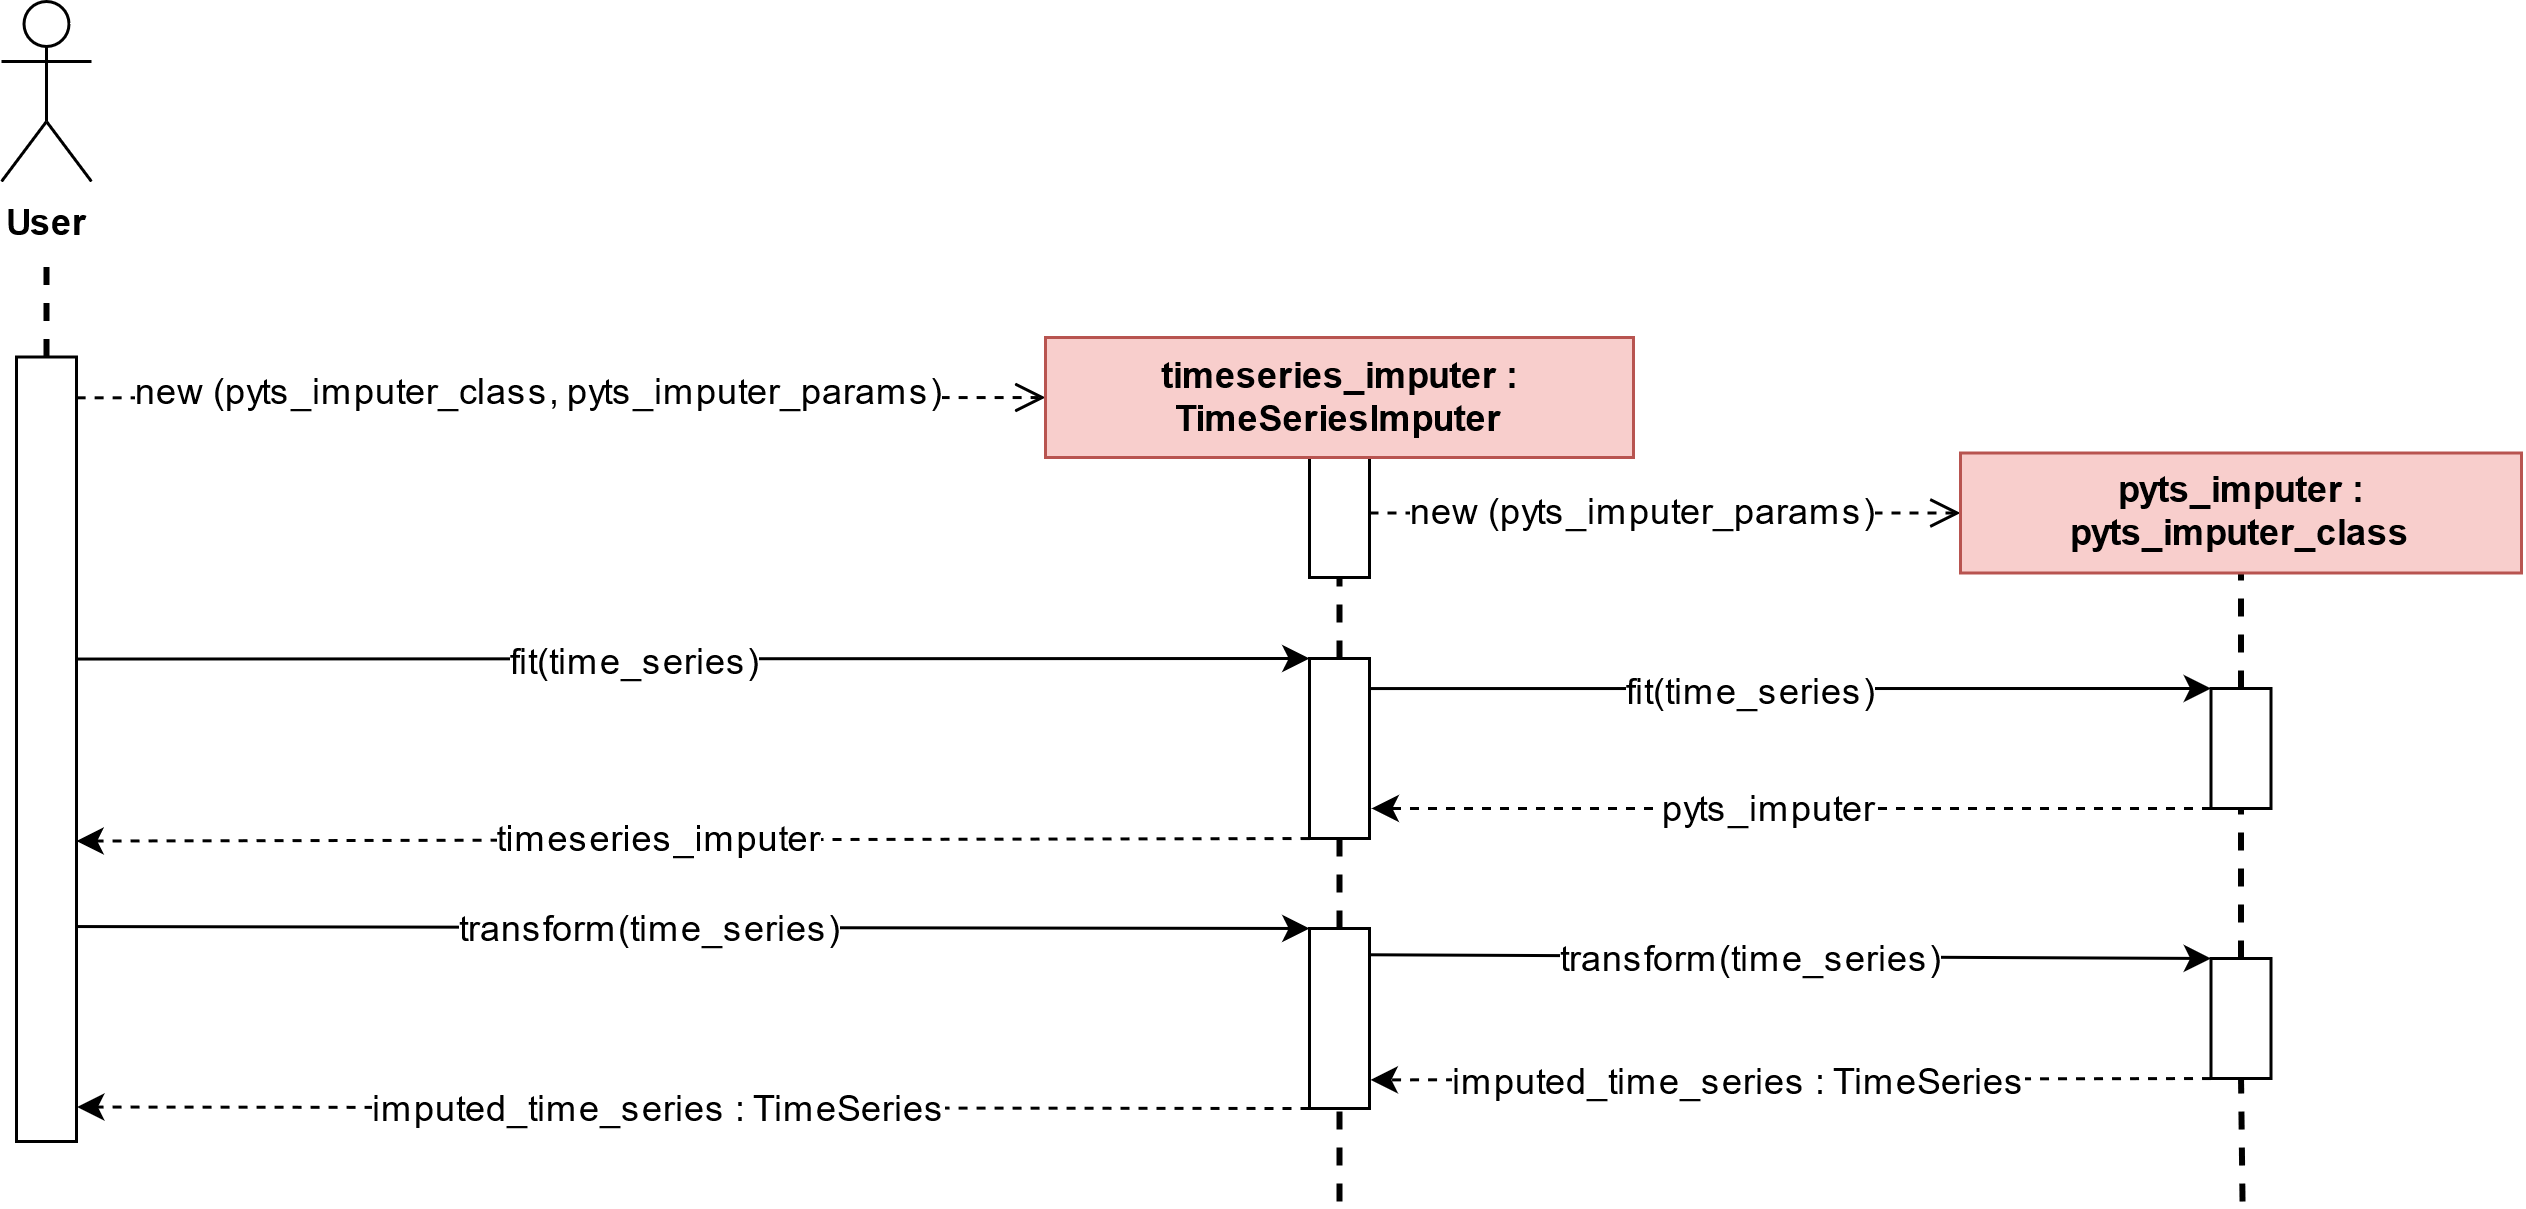
\includegraphics[width=\textwidth]{gfx/pyts_imputer_sequence}
    \caption{Sequence Diagram of the PytsImputeWrapper class for fit and transform use-case.}
    \label{fig:tfe-pyts-impute-seq}s
\end{figure}
\subsubsection*{PytsTransformWrapper}
\vspace*{-10mm}\hfill{\fontfamily{phv}\normalsize\emph{Paul Fährmann and Sanjay Gupta}}
\\
The \textit{PytsTransformWrapper} is a wrapper for the \textit{pyts.transform}\footnote{\href{https://pypi.org/project/pyts/}{https://pypi.org/project/pyts/}} classes. We specify the class and the constructor params of the transformer class in the \textit{PytsTransformWrapper} constructor and create the \textit{pyts\_transformer\_class} object with the specified params. In Figure~\ref{fig:tfe-pyts-transform-seq}, we show the use case for the fit and the transform function call. In the \textit{fit} call we call the fit function of that transformer and get back the \textit{pyts\_transformer}. In the \textit{transform} call we just call the transform function of the transformer class object.
\begin{figure}[ht]
    \centering
    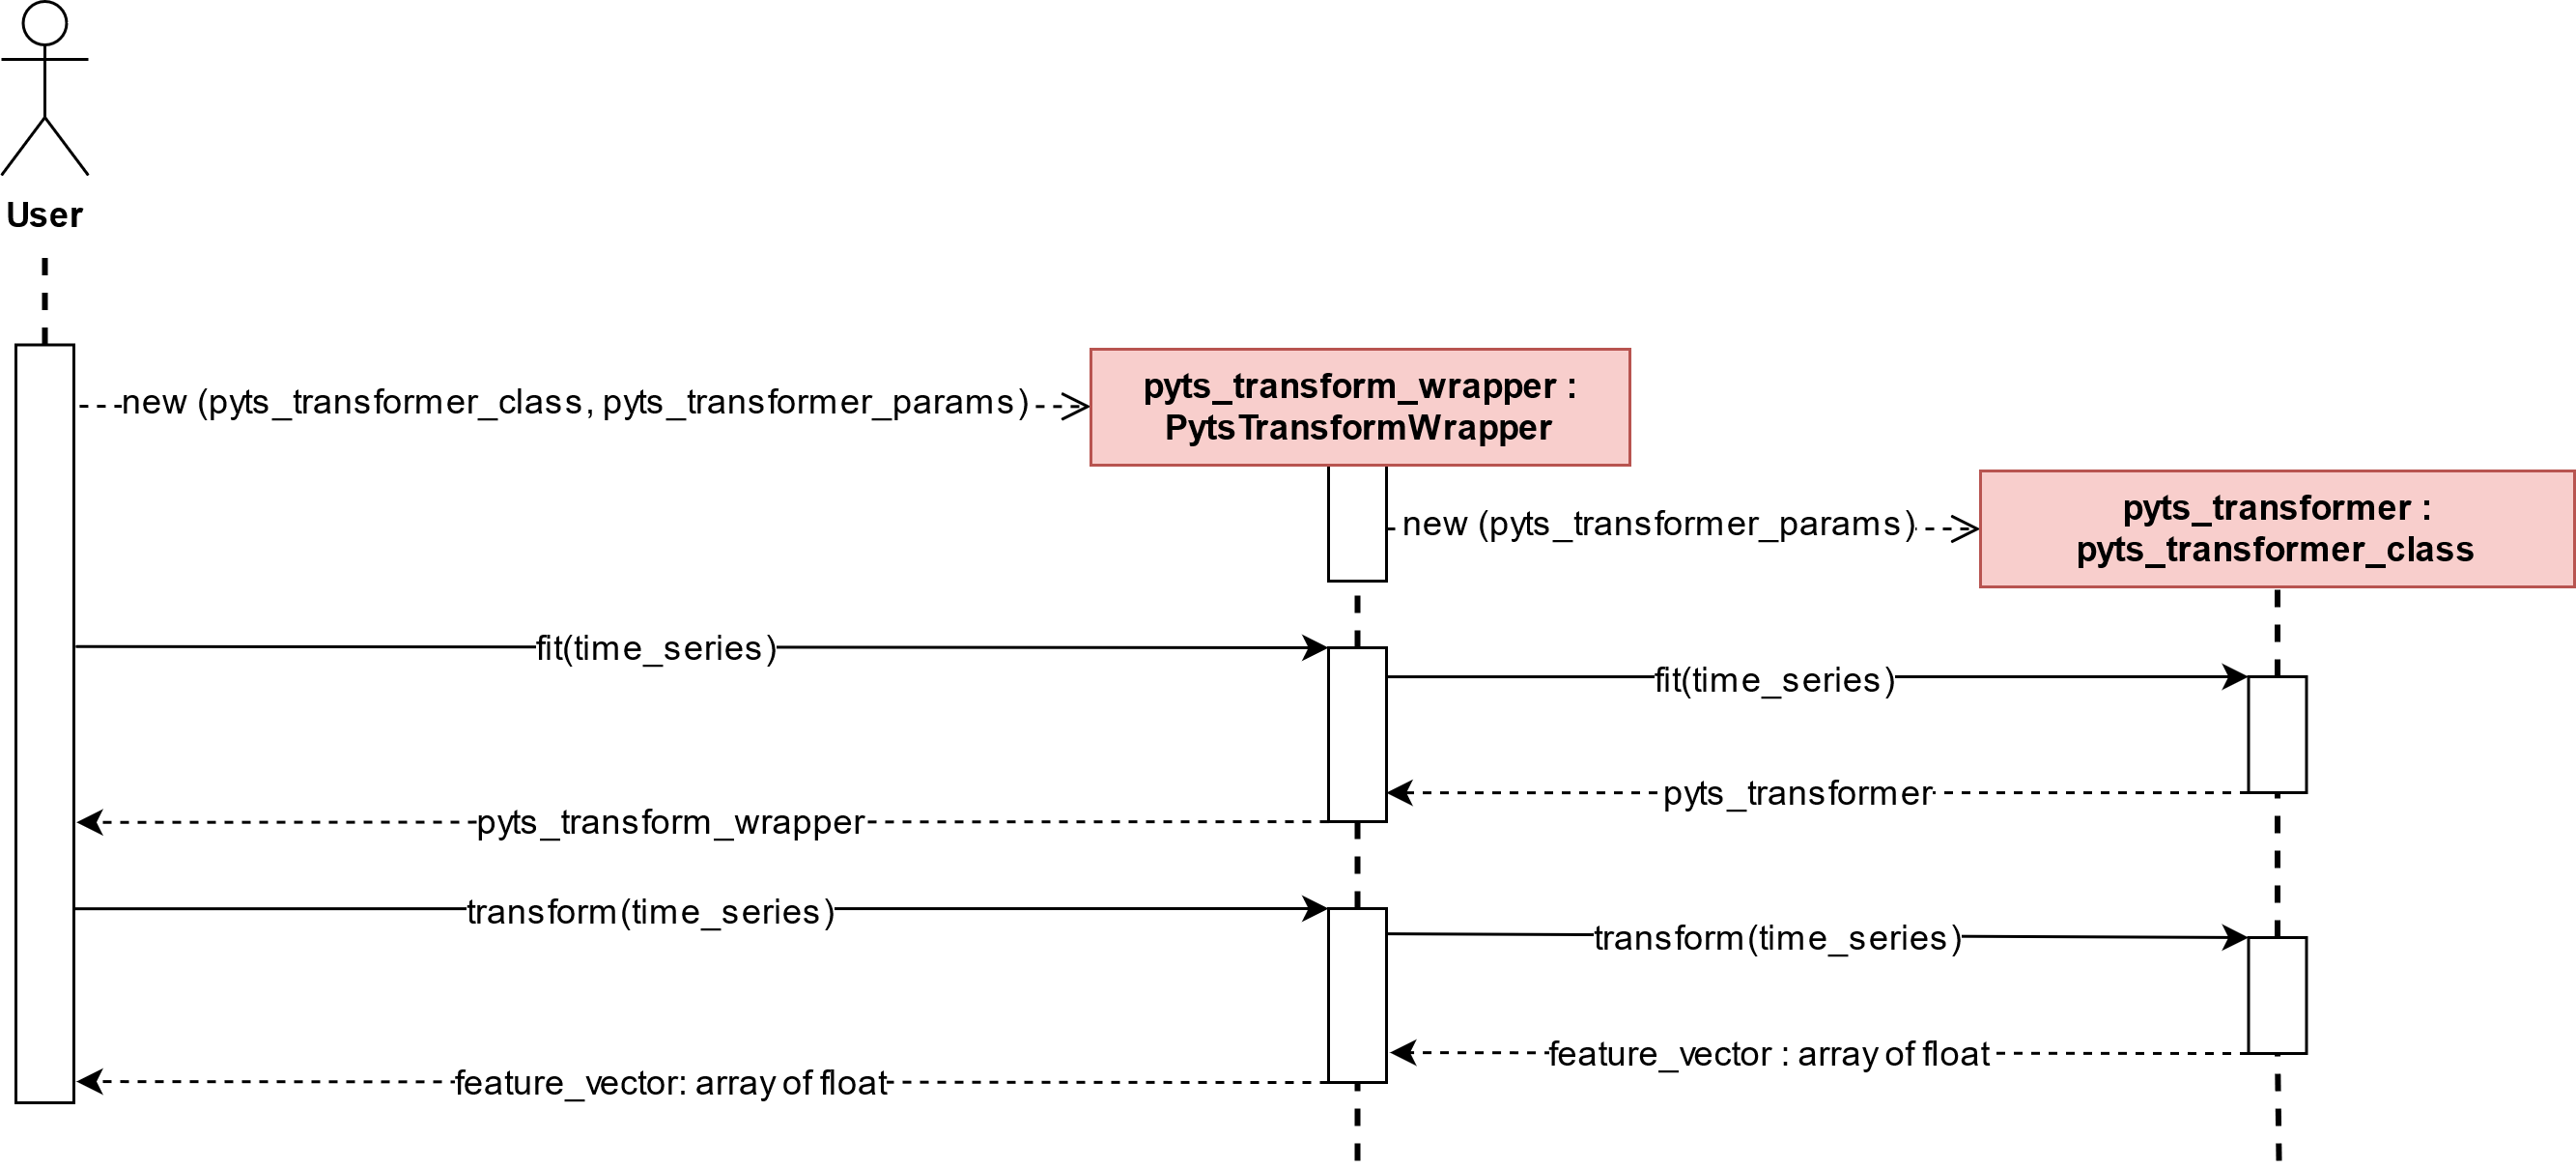
\includegraphics[width=\textwidth]{gfx/pyts_transform_sequence}
    \caption{Sequence Diagram of the PytsTransformWrapper class for fit and transform use-case.}
    \label{fig:tfe-pyts-transform-seq}
\end{figure}
\\
Figure \ref{fig:pyts-transform-wrapper-seq} show the use case for the fit and the transform function call with the ROCKET, Bag of Patterns, and Shapelet Transform. To access all the methods of \textit{pyts.transformation} class, we first need to initialize the \textit{pyts.transformation} class. From the \textit{PytsTransformeWrapper} class we can directly call the ROCKET, Bag of Patterns, and Shapelet Transform method which all return model as an object. Then we use this model to fit our time series data and transform the data. After fitting the Bag of Patterns model with the dataset it will give word frequencies for each time series. The \textit {fit\_transform} method of Shapelet Transform method return the feature vectors.
\begin{figure}[ht]
    \centering
    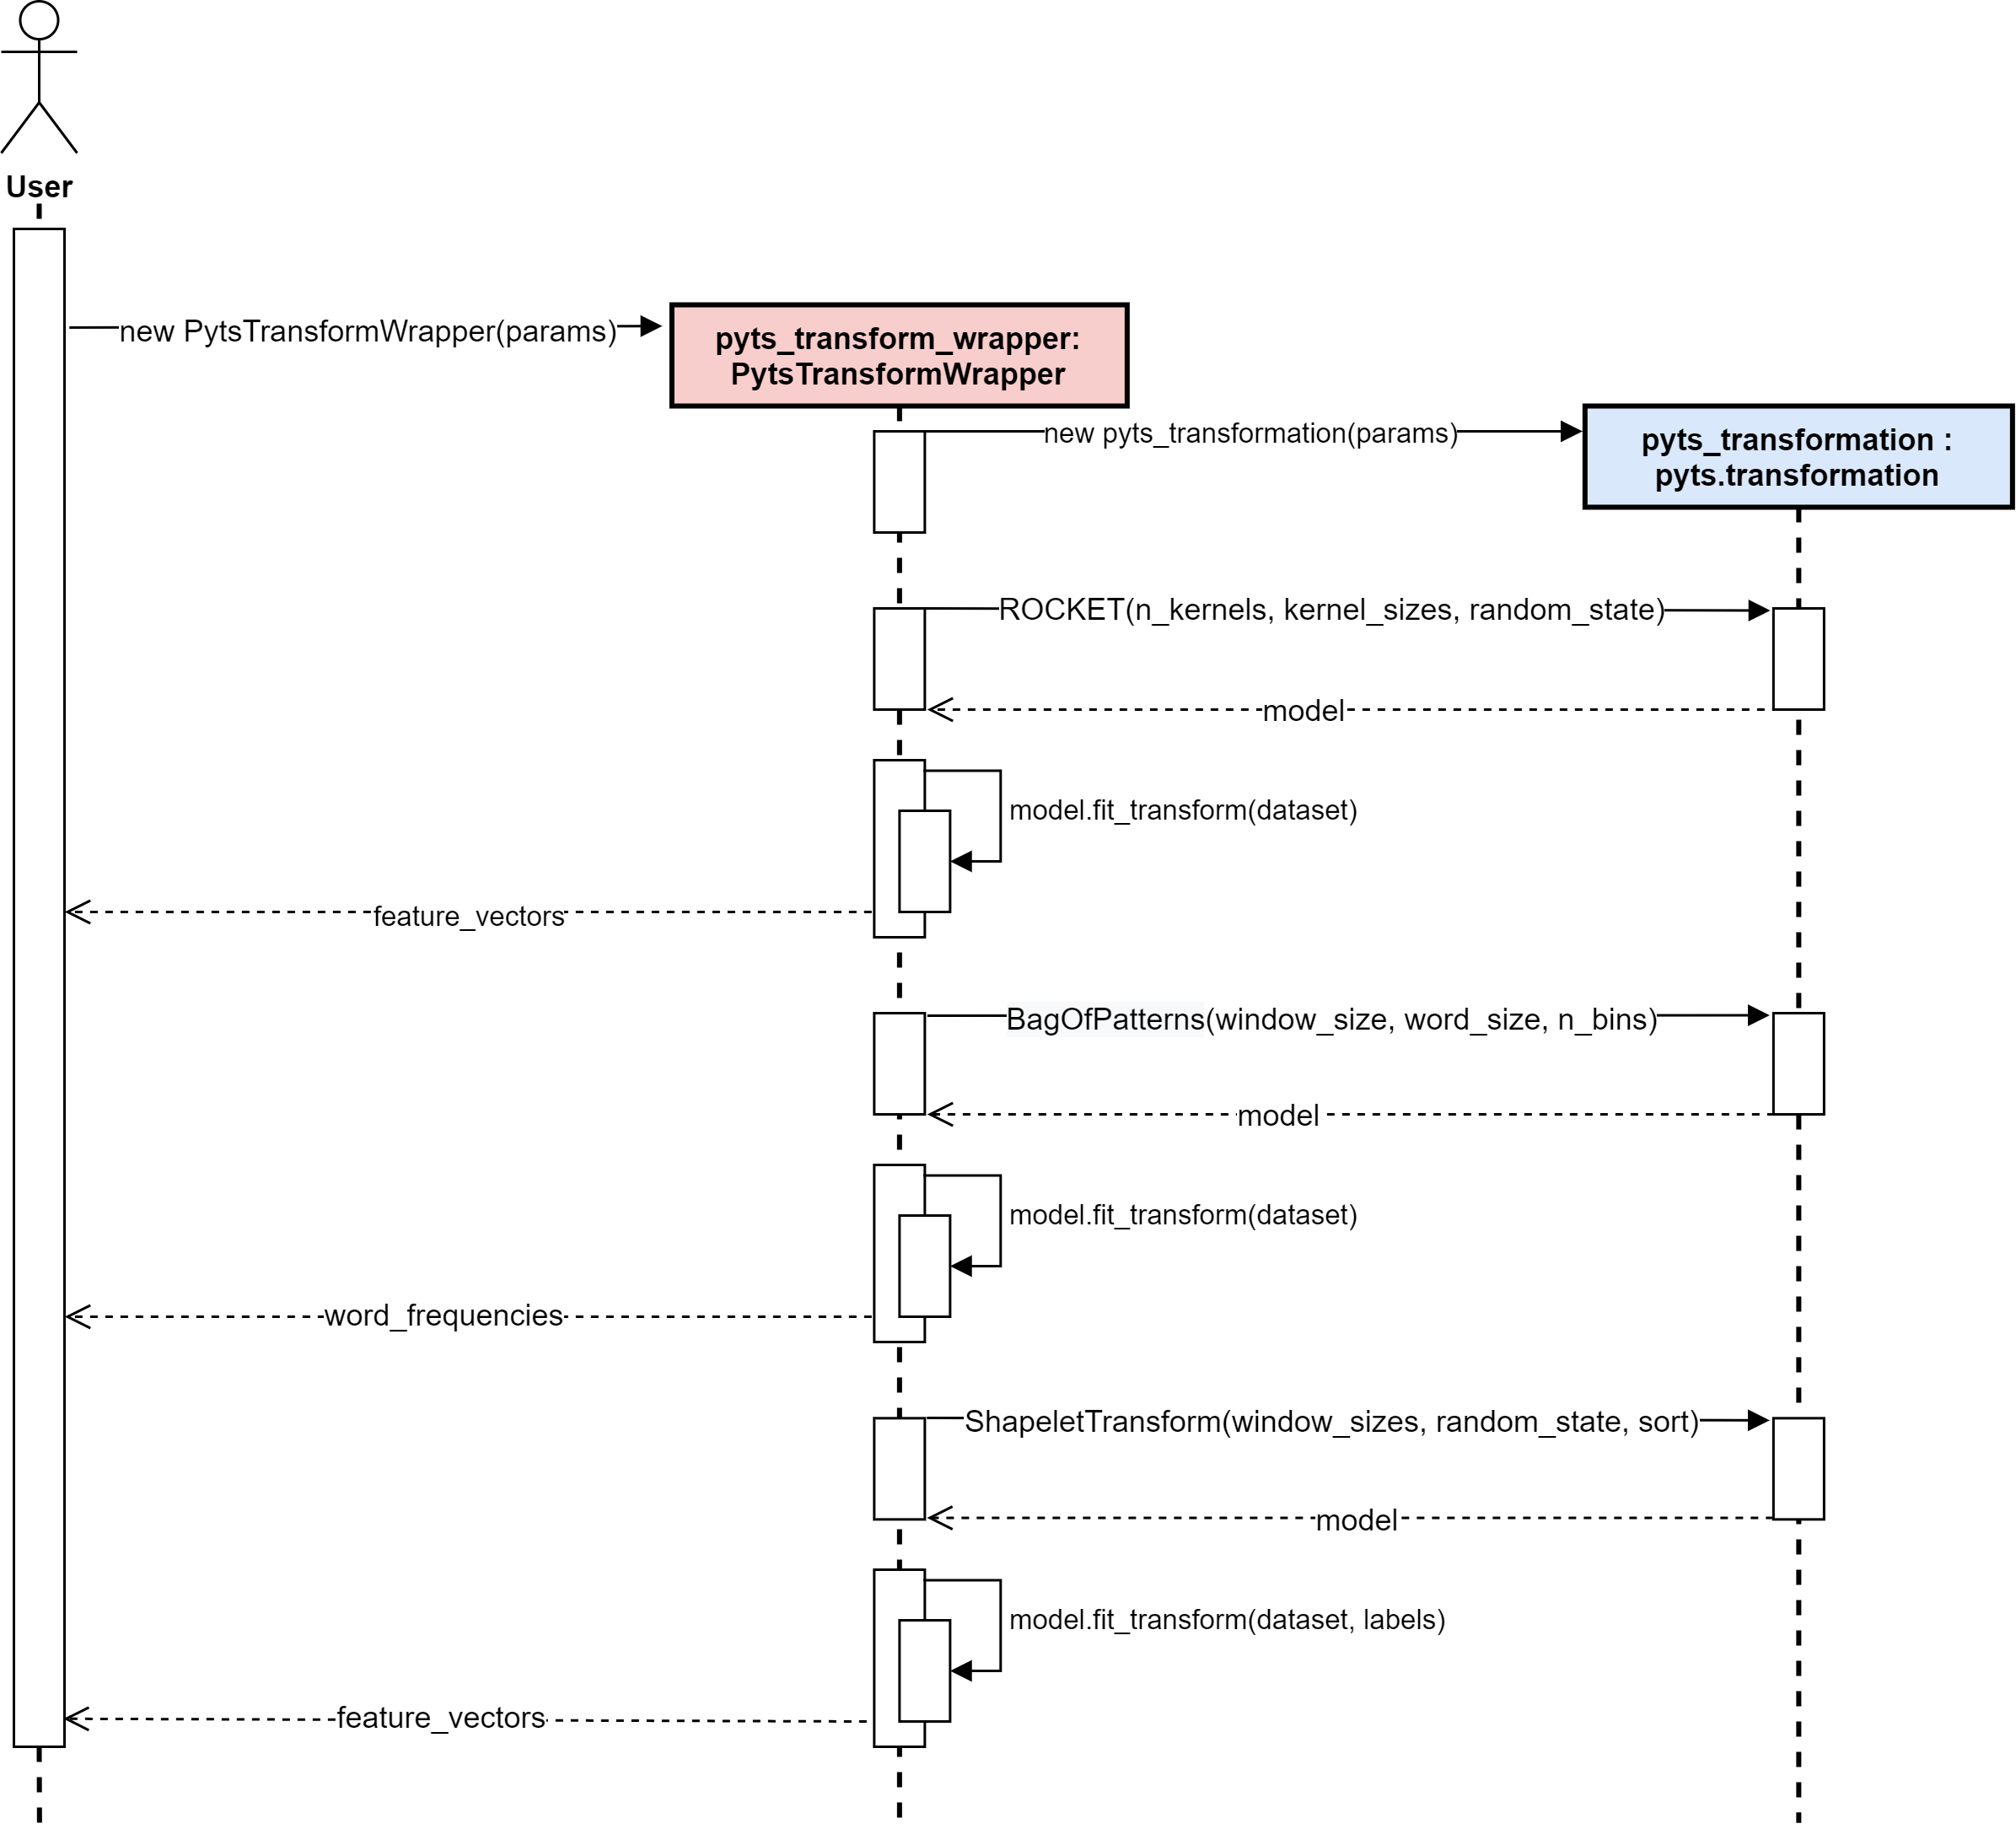
\includegraphics[width=\textwidth]{gfx/pyts_transform_wrapper-Sequence.png}
    \caption{Sequence Diagram of the PytsTransformWrapper class with ROCKET, BOP, and Shapelet Transform for fit and transform use-case.}
    \label{fig:pyts-transform-wrapper-seq}
\end{figure}
\subsubsection*{TSFreshWrapper}
\vspace*{-10mm}\hfill{\fontfamily{phv}\normalsize\emph{Sanjay Gupta}}
\\
The \textit{TSFreshWrapper} is a wrapper for the \textit{tsfresh} \footnote{\href{https://pypi.org/project/tsfresh/}{https://pypi.org/project/tsfresh/}} Package. The \textit{tsfresh} stands for Time Series Feature extraction based on scalable hypothesis tests. The package contains many feature extraction methods and feature selection algorithms. In Figure \ref{fig:tsfresh-wrapper-seq}, we show the use case for the fit and the transform function call. To access all the classes related to feature engineering we need to first initialize the \textit{tsfresh} package. The \textit{tsfresh.feature\_extraction.feature\_calculators} module contains more than sixty features or methods that take time series data as input and calculate the values of the feature.
\begin{figure}[ht]
    \centering
    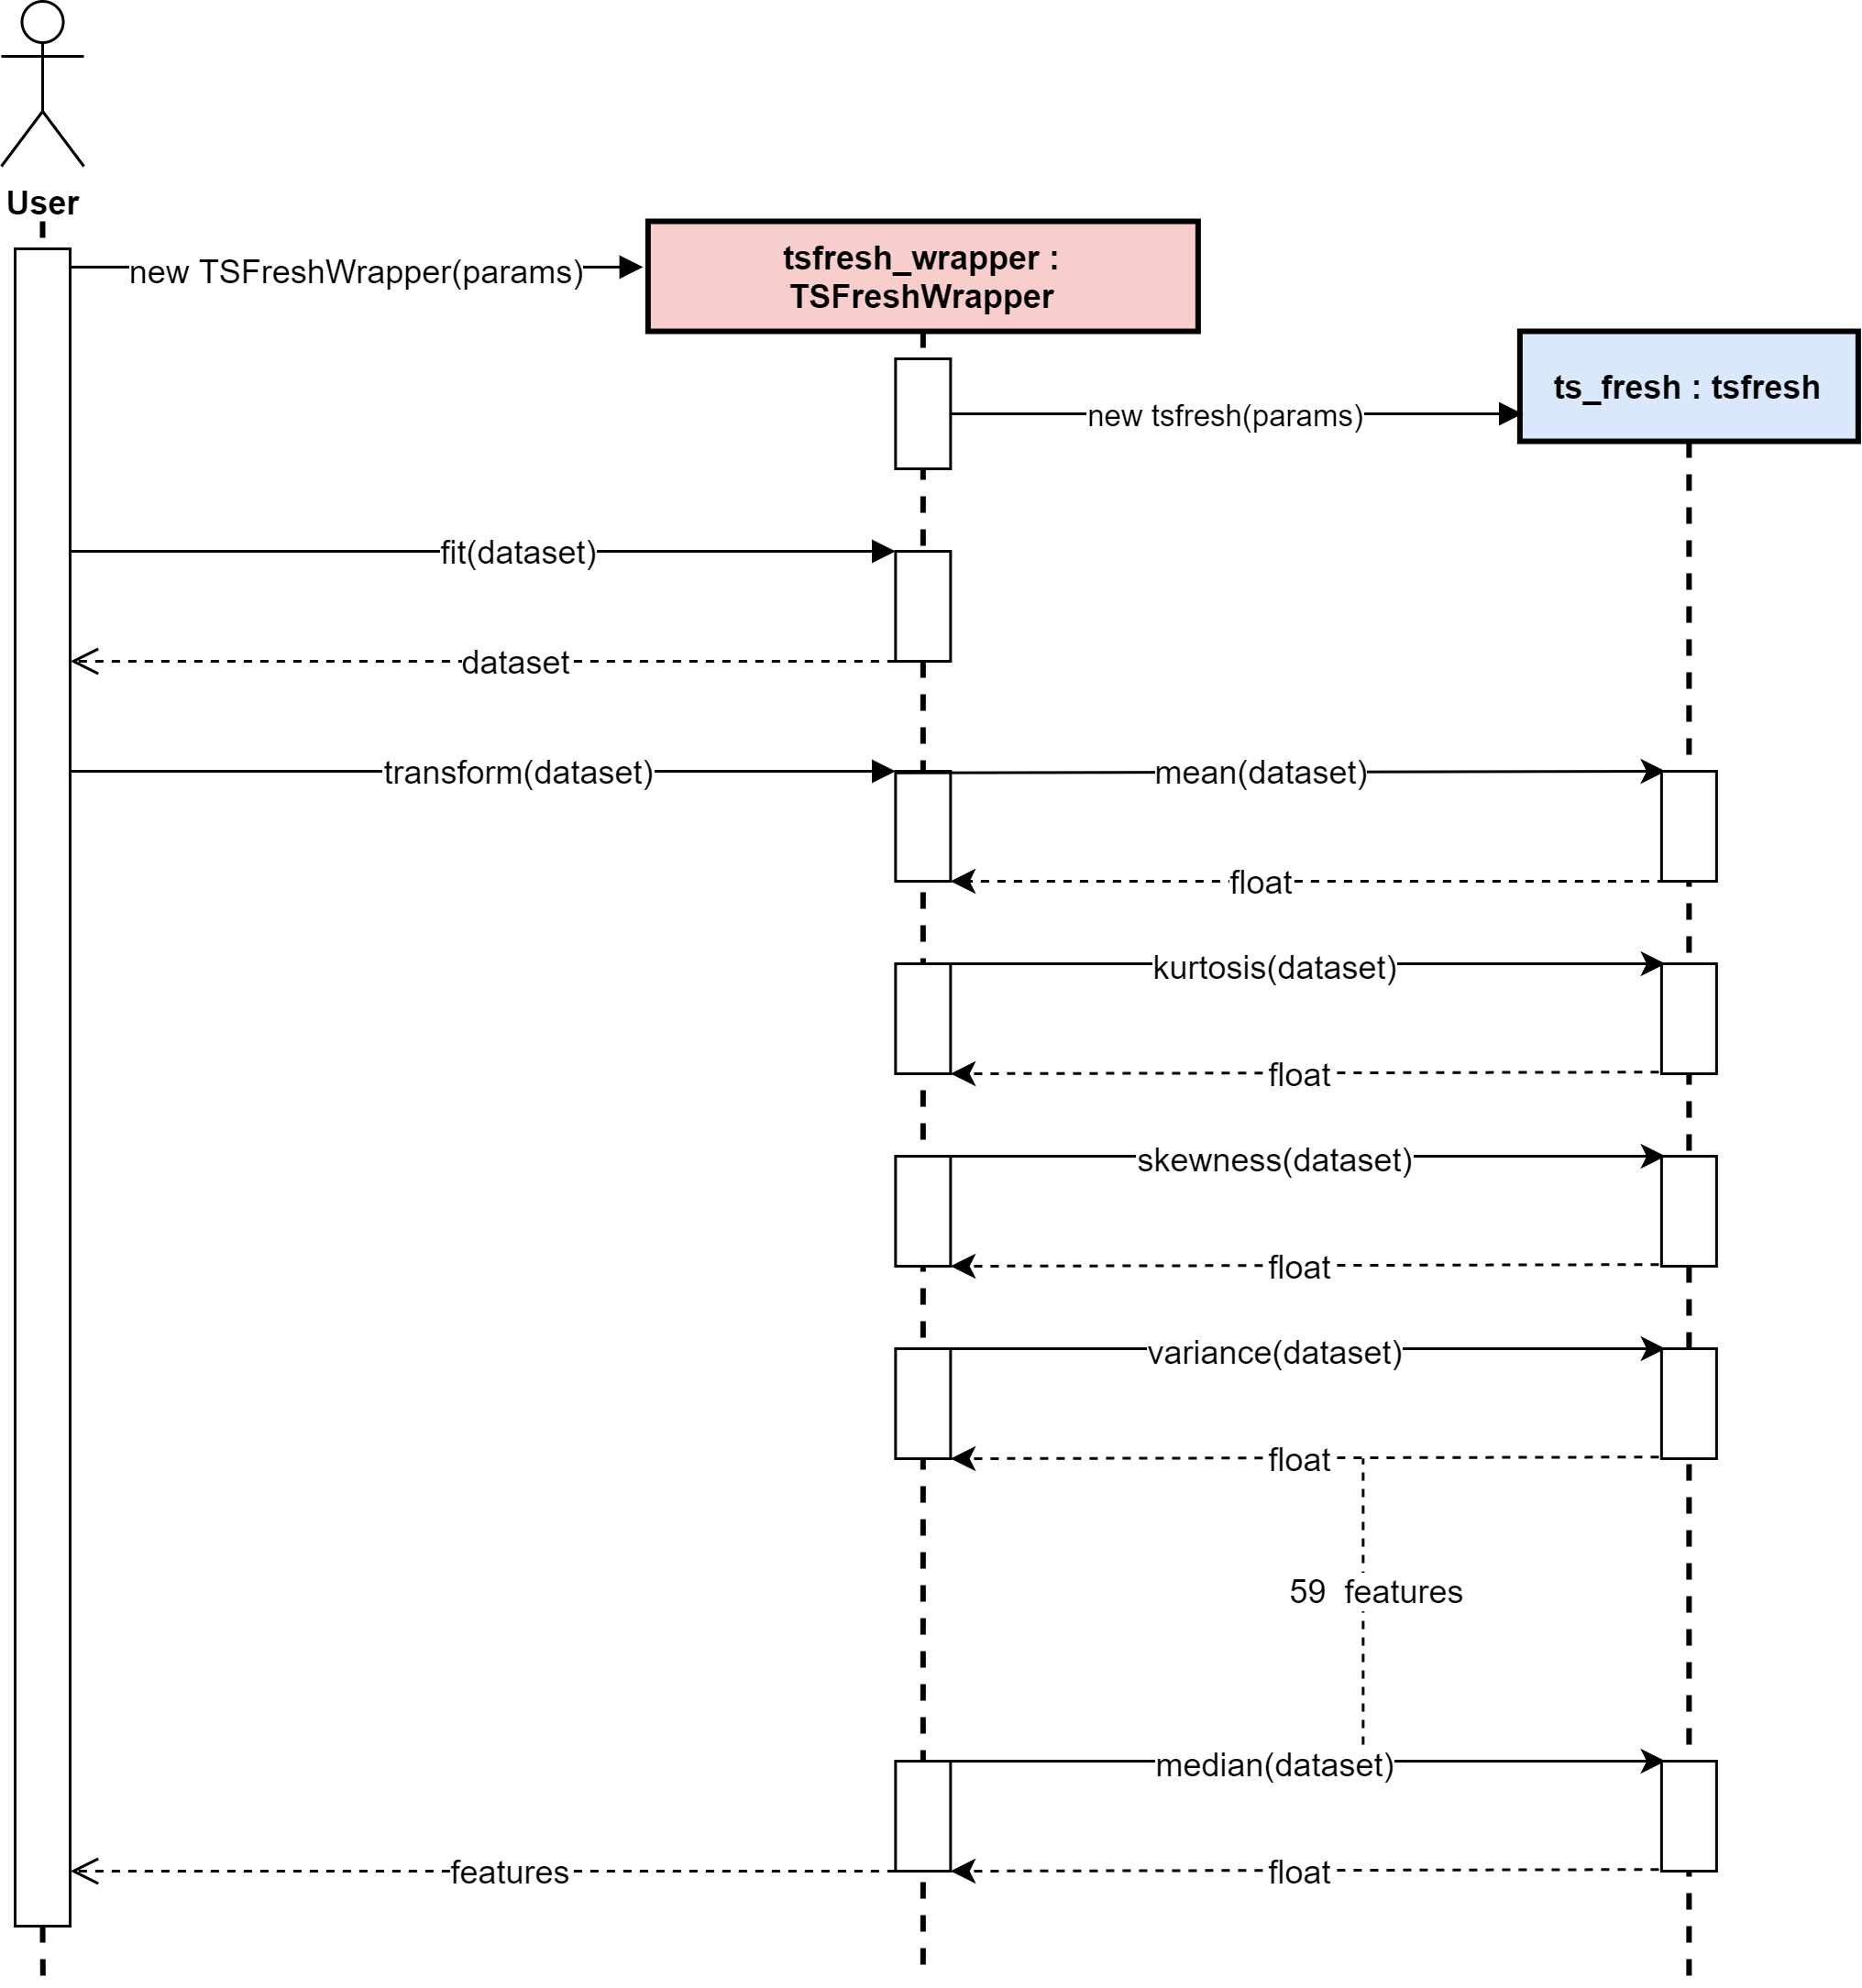
\includegraphics[width=\textwidth]{gfx/TSFreshWrapper-Sequence}
    \caption{Sequence Diagram of the TSFreshWrapper class for fit and transform use-case.}
    \label{fig:tsfresh-wrapper-seq}
\end{figure}
\subsubsection*{RNNAutoencoder}
\vspace*{-10mm}\hfill{\fontfamily{phv}\normalsize\emph{Sanjay Gupta}}
\\
The \textit{RNNAutoencoder} class use \textit{tensorflow} \footnote{\href{https://pypi.org/project/tensorflow/}{https://pypi.org/project/tensorflow/}} library to perform the RNN and Autoencoder functionality. Tensorflow is a open source software library for high-performance numerical computation. In Figure \ref{fig:rnn-seq}, we show the use case for the fit and the transform function call. To access all the classes which is required to implement RNN can be directly call in \textit{RNNAutoencoder} class after initialization of \textit{tensorflow} library. The \textit{RNNAutoencoder} class will return the feature vector as a output for the \textit{transform} call.
\begin{figure}[ht]
    \centering
    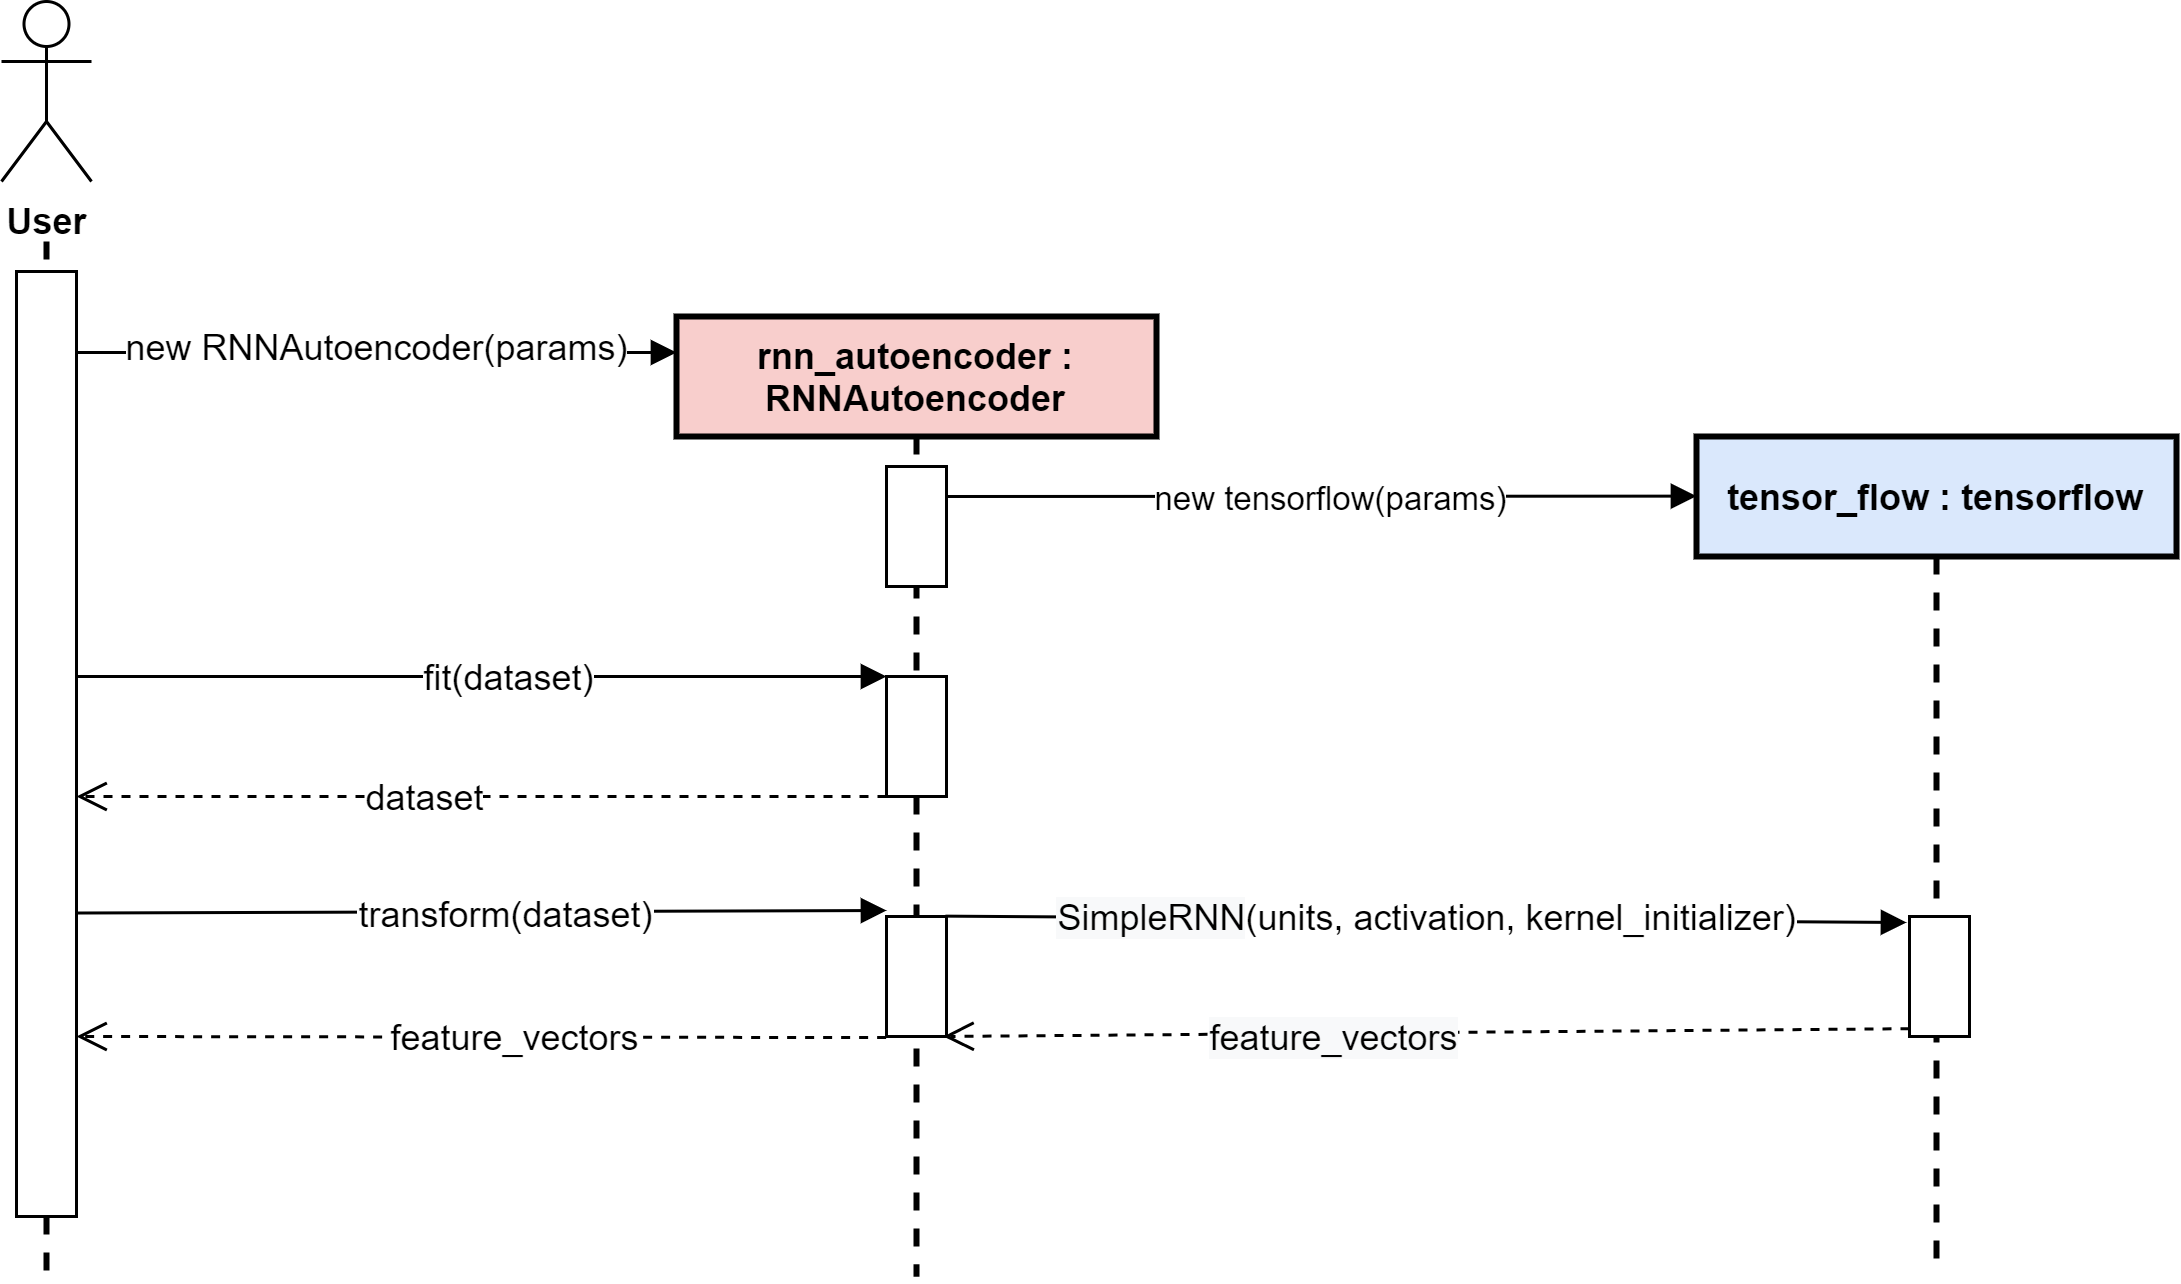
\includegraphics[width=\textwidth]{gfx/RNN-Sequence}
    \caption{Sequence Diagram of the RNN Autoencoder for fit and transform use-case.}
    \label{fig:rnn-seq}
\end{figure}
\subsubsection*{WindowingApproach}
\vspace*{-10mm}\hfill{\fontfamily{phv}\normalsize\emph{Sanjay Gupta}}
\\
The \textit{WindowingApproach} class use \textit{sklearn} \footnote{\href{https://pypi.org/project/scikit-learn/}{https://pypi.org/project/scikit-learn/}} module to perform the windowing transformation. The \textit{sklearn} is a python module for machine learning built on top of \textit{SciPy} \footnote{\href{https://www.scipy.org/}{https://www.scipy.org/}}. Using \textit{sklearn} library, we can perform classification, regression, clustering, dimensionality reduction, model selection, and preprocessing operation on datasets. In Figure \ref{fig:rnn-seq}, we show the use case for the fit and the transform function call. We can access all the classes and method of \textit{sklearn} module by initializing library in \textit{WindowingApproach} class. The \textit{WindowingApproach} class will return the window for each time series as a output for the \textit{transform} call.
\begin{figure}[ht]
    \centering
    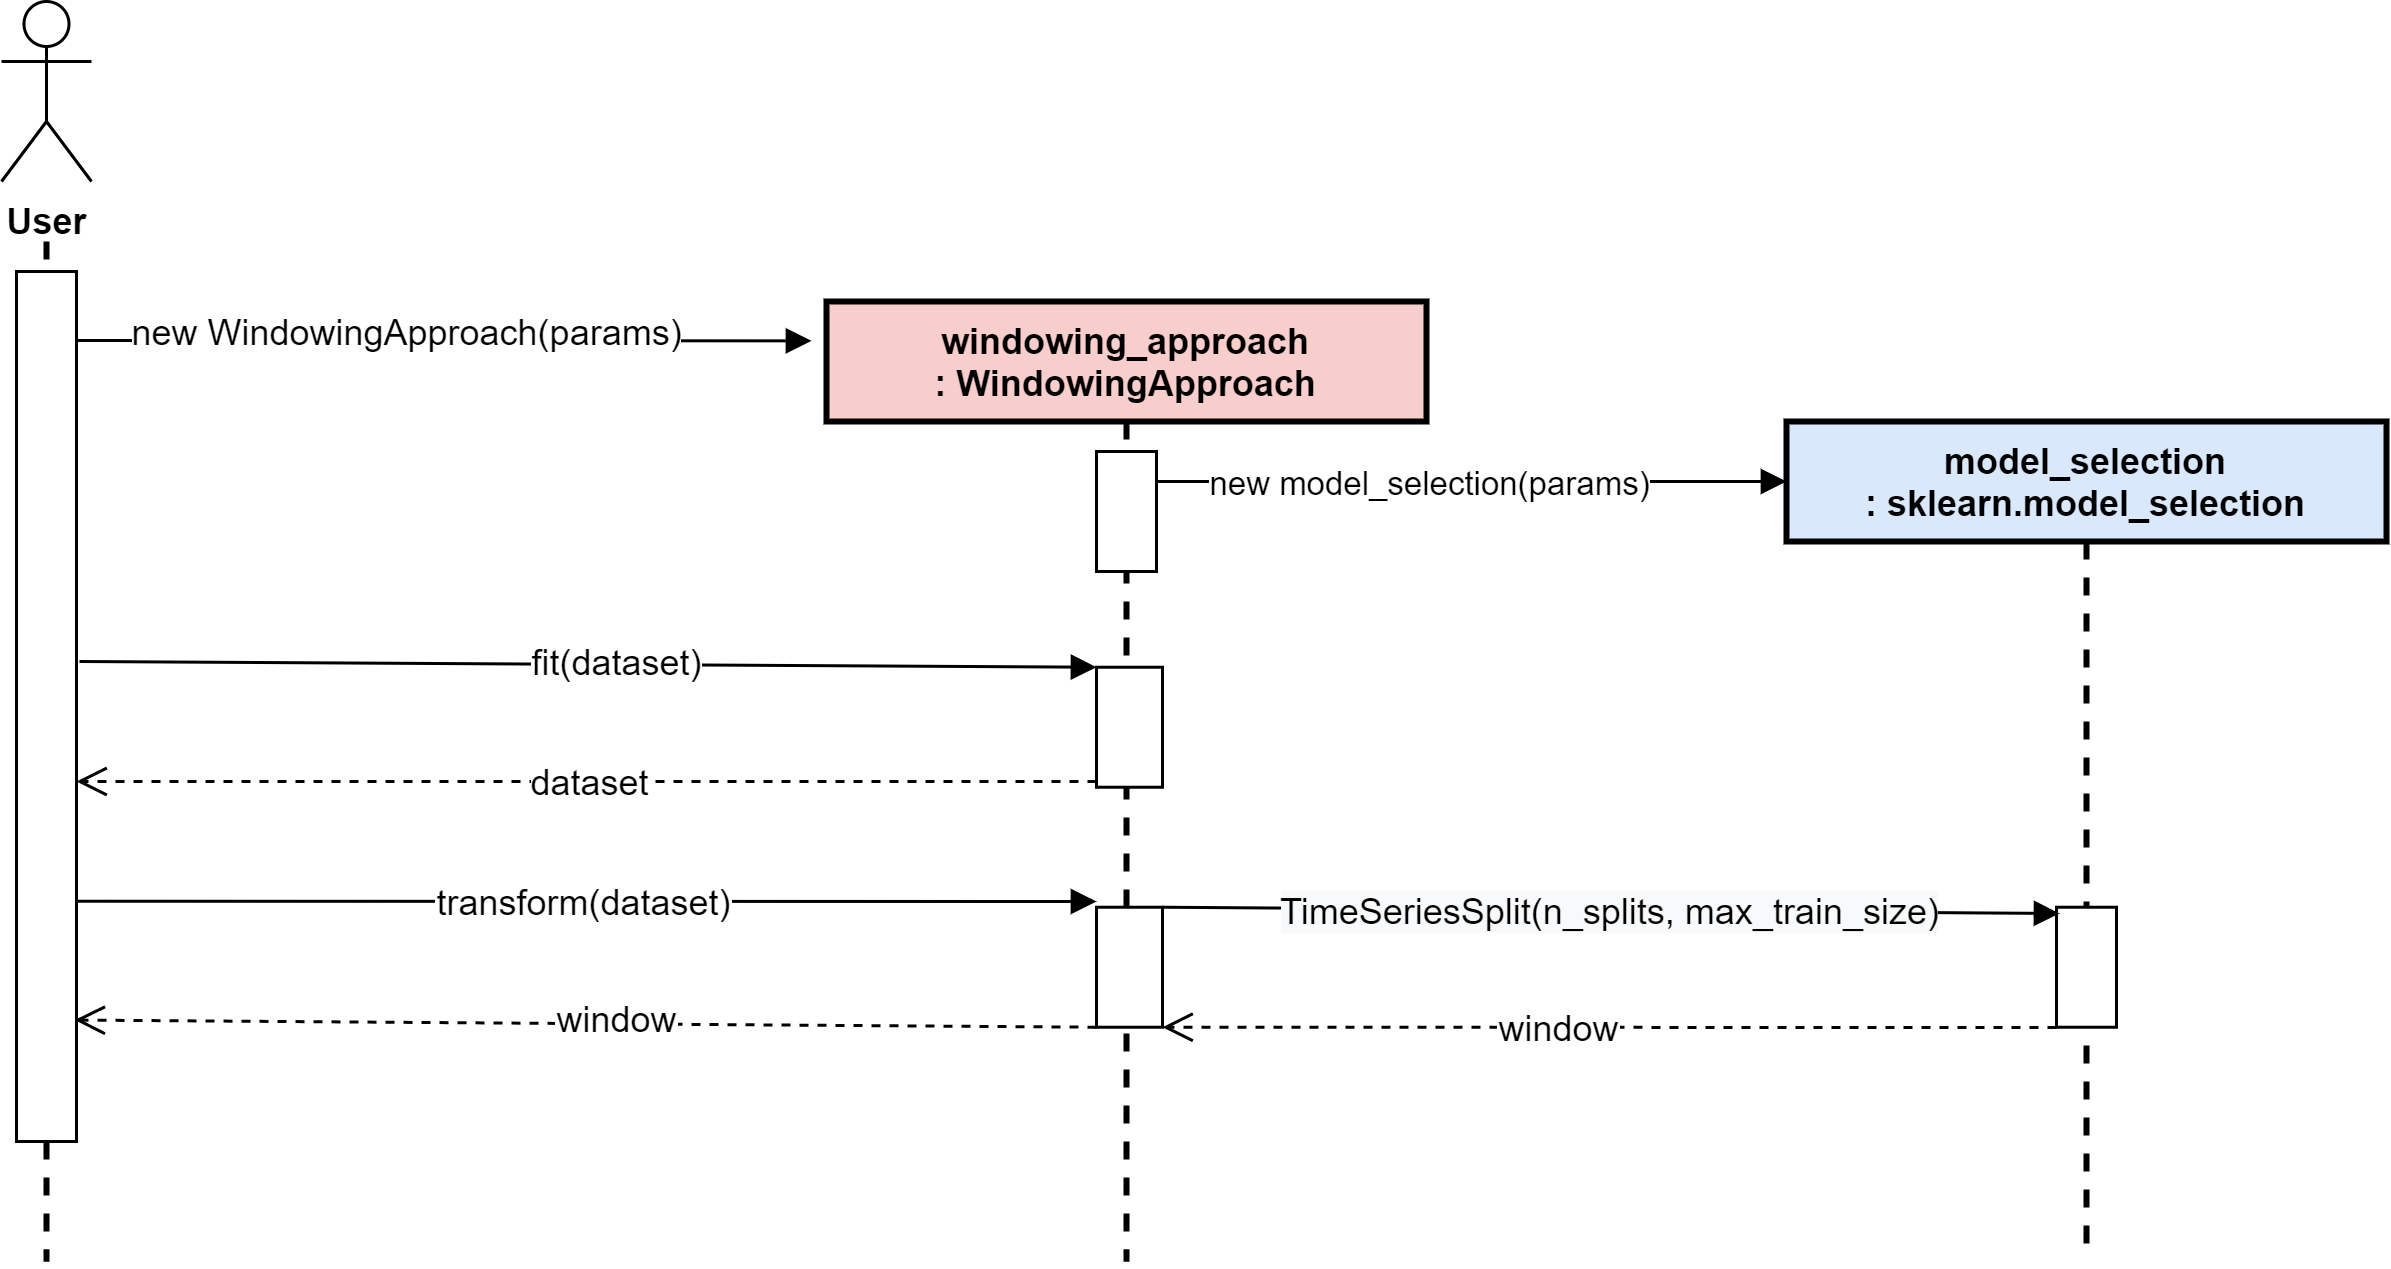
\includegraphics[width=\textwidth]{gfx/WindowApproach-Sequence}
    \caption{Sequence Diagram of the Windowing Approach for fit and transform use-case.}
    \label{fig:window-seq}
\end{figure}

\newpage
\section{Health Index Estimation}
\vspace*{-15mm}\hfill{\fontfamily{phv}\normalsize\emph{Selami Hoxha}}
\label{sec:system_design:health_index}

In this section the design for the health index estimation module of the framework is presented, starting with the class diagram and then
presenting sequence diagrams for the approaches that will be implemented.

\subsection*{Class diagram}
The class diagram of health index builds on the general class diagram. It extends the general class diagram by extending the HealthIndexEstimator abstract class.
In this module three approaches are presented with three purple box classes. The approaches use make use of different libraries like scikit-learn, tensorflow and scipy as shown
in the figure \ref{fig:class_hie}. In health index estimation also a Transformer abstract class from the general class diagram is used which will help with
feature extraction and other data transformation that are needed.
\begin{figure}[H]
    \centering
    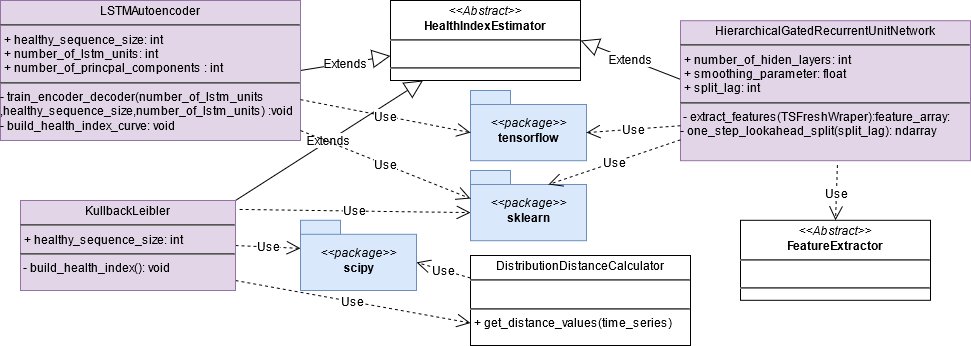
\includegraphics[width=\textwidth]{gfx/Interfaces-HIE.png}
    \caption{Class diagram for health index estimation module}
    \label{fig:class_hie}
\end{figure}

\subsection*{Sequence diagram}
The sequence diagrams try to show the flow of the approaches by showing the interactions between different classes. The sequence
diagrams for three approaches are presented in the figures \ref{fig:sequence_lstm}, \ref{fig:sequence_hgrun} and \ref{fig:sequence_KLD}.

\begin{figure}[H]
    \centering
    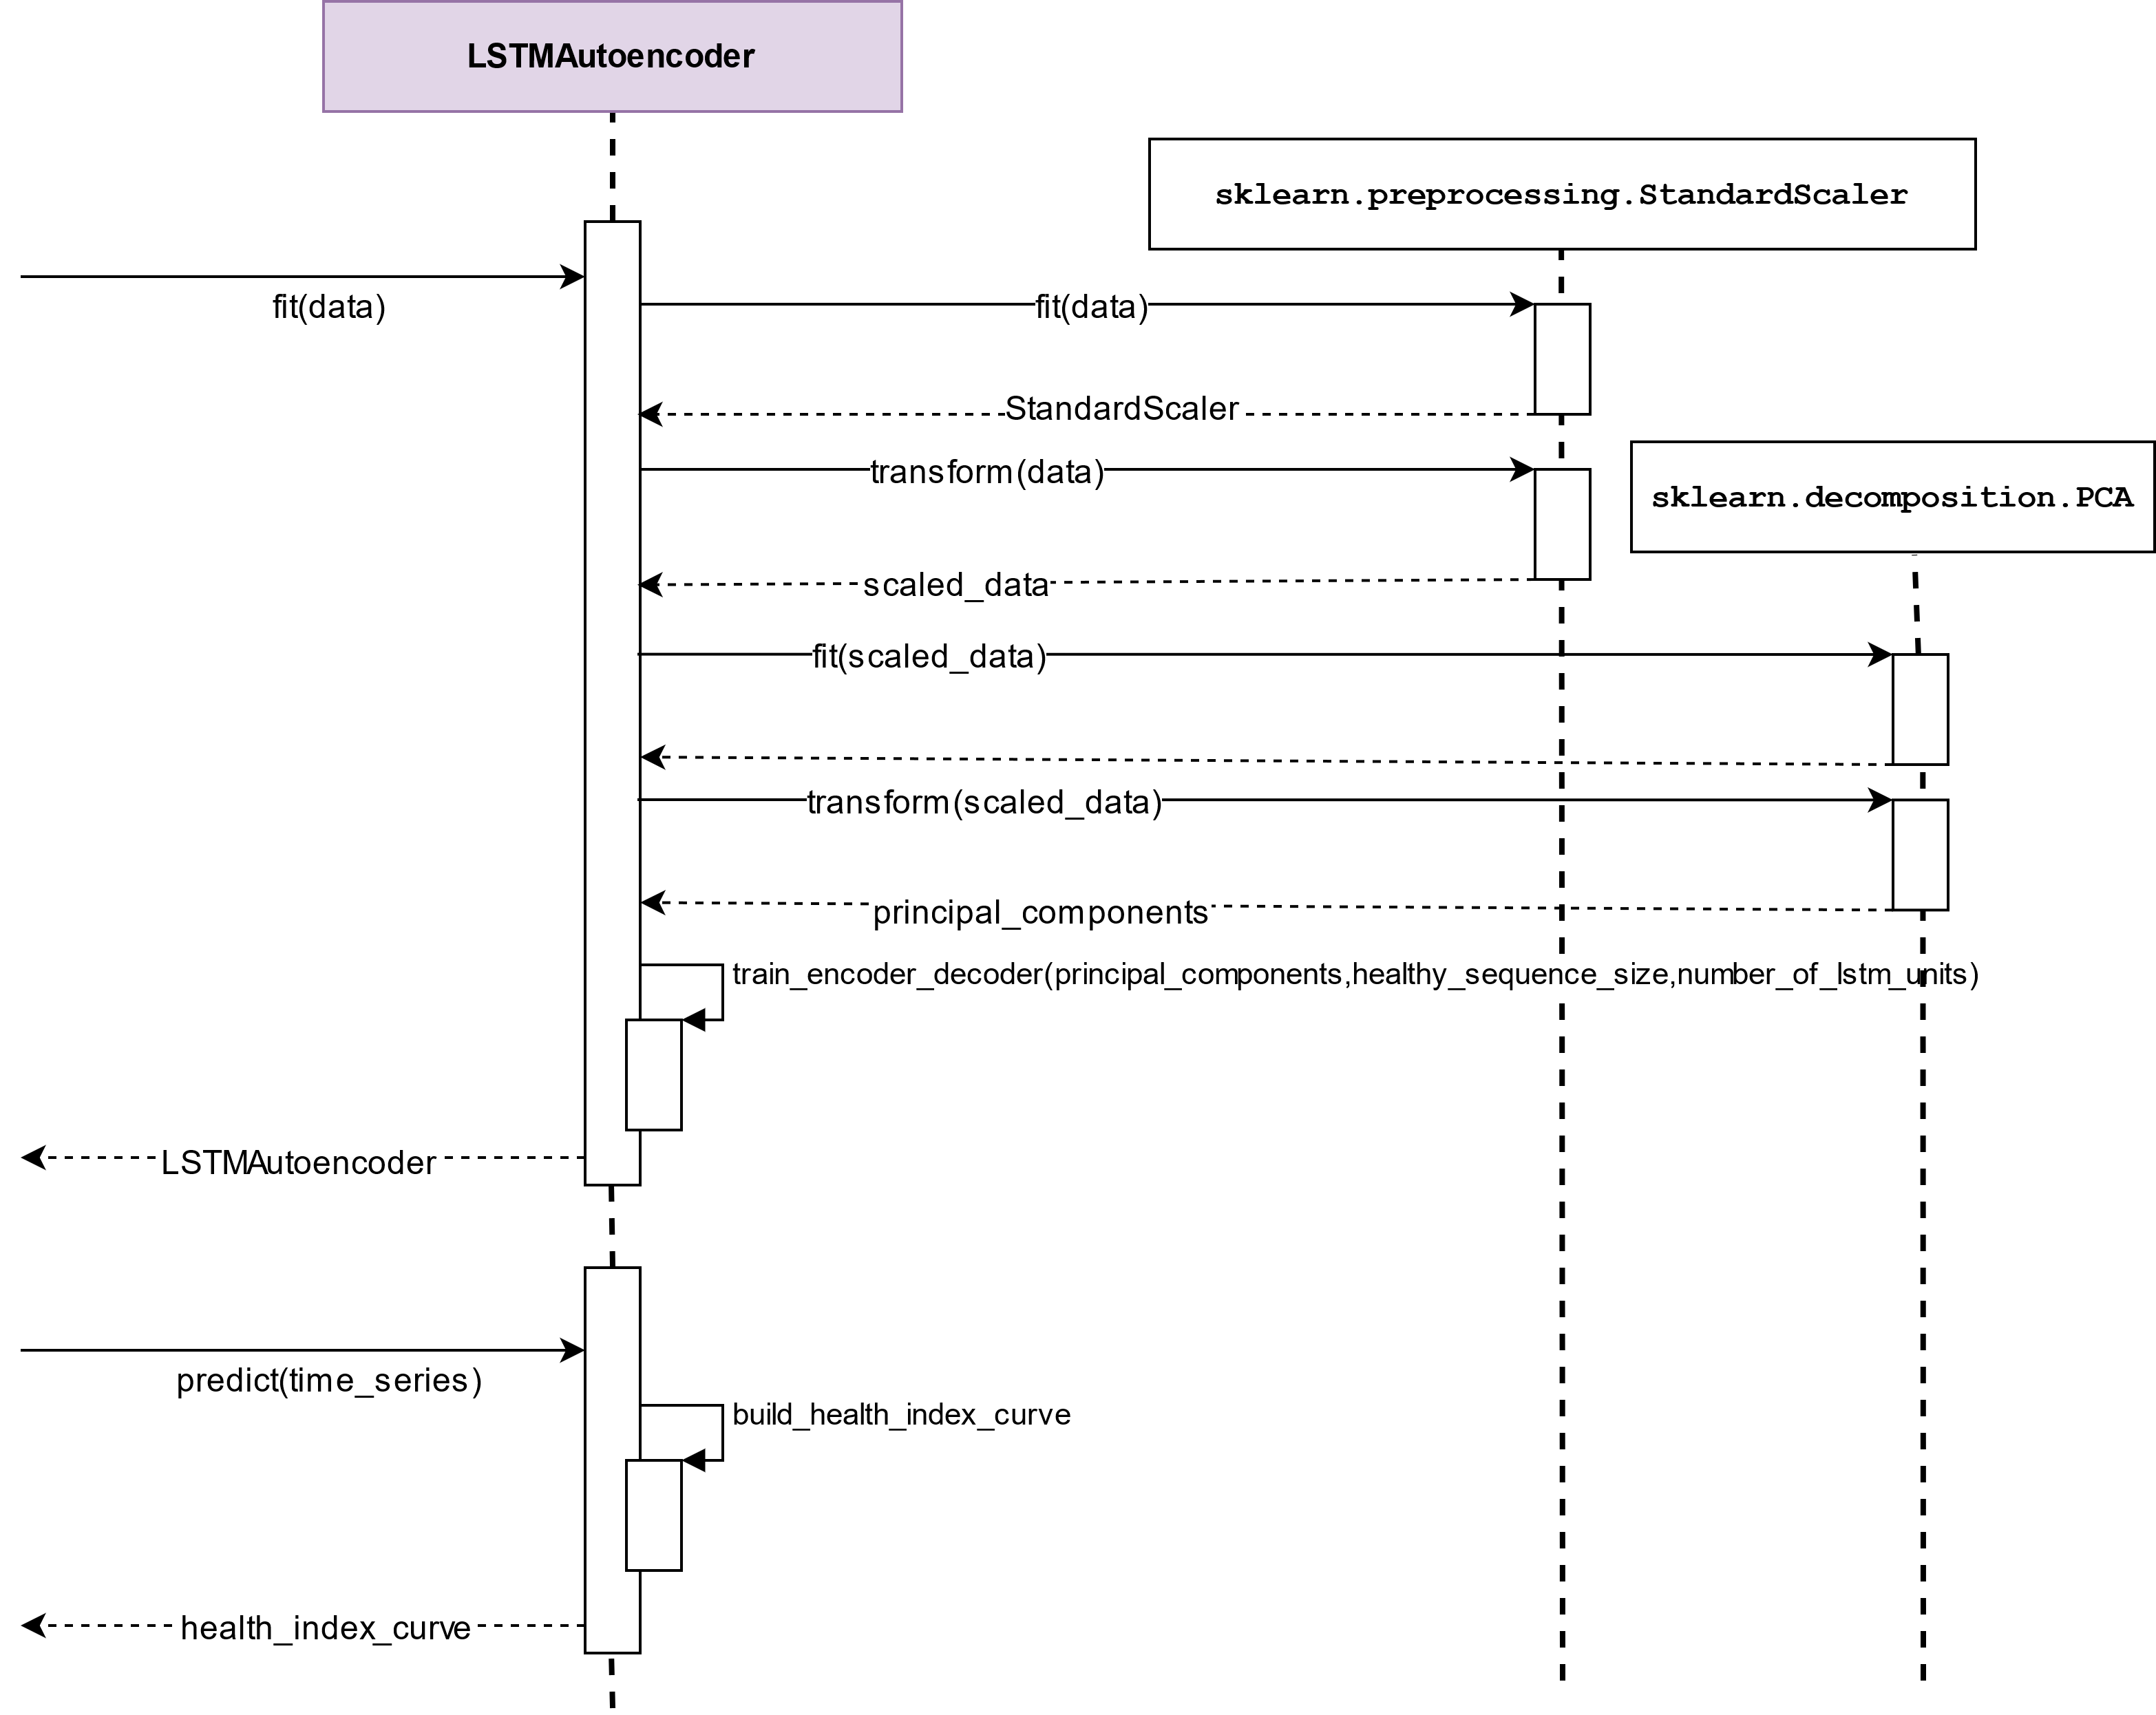
\includegraphics[width=\textwidth]{gfx/LSTMatuoencodersequencediagram.png}
    \caption{LSTM Encoder-Decoder HI estimation sequence diagram}
    \label{fig:sequence_lstm}
\end{figure}

\begin{figure}[H]
    \centering
    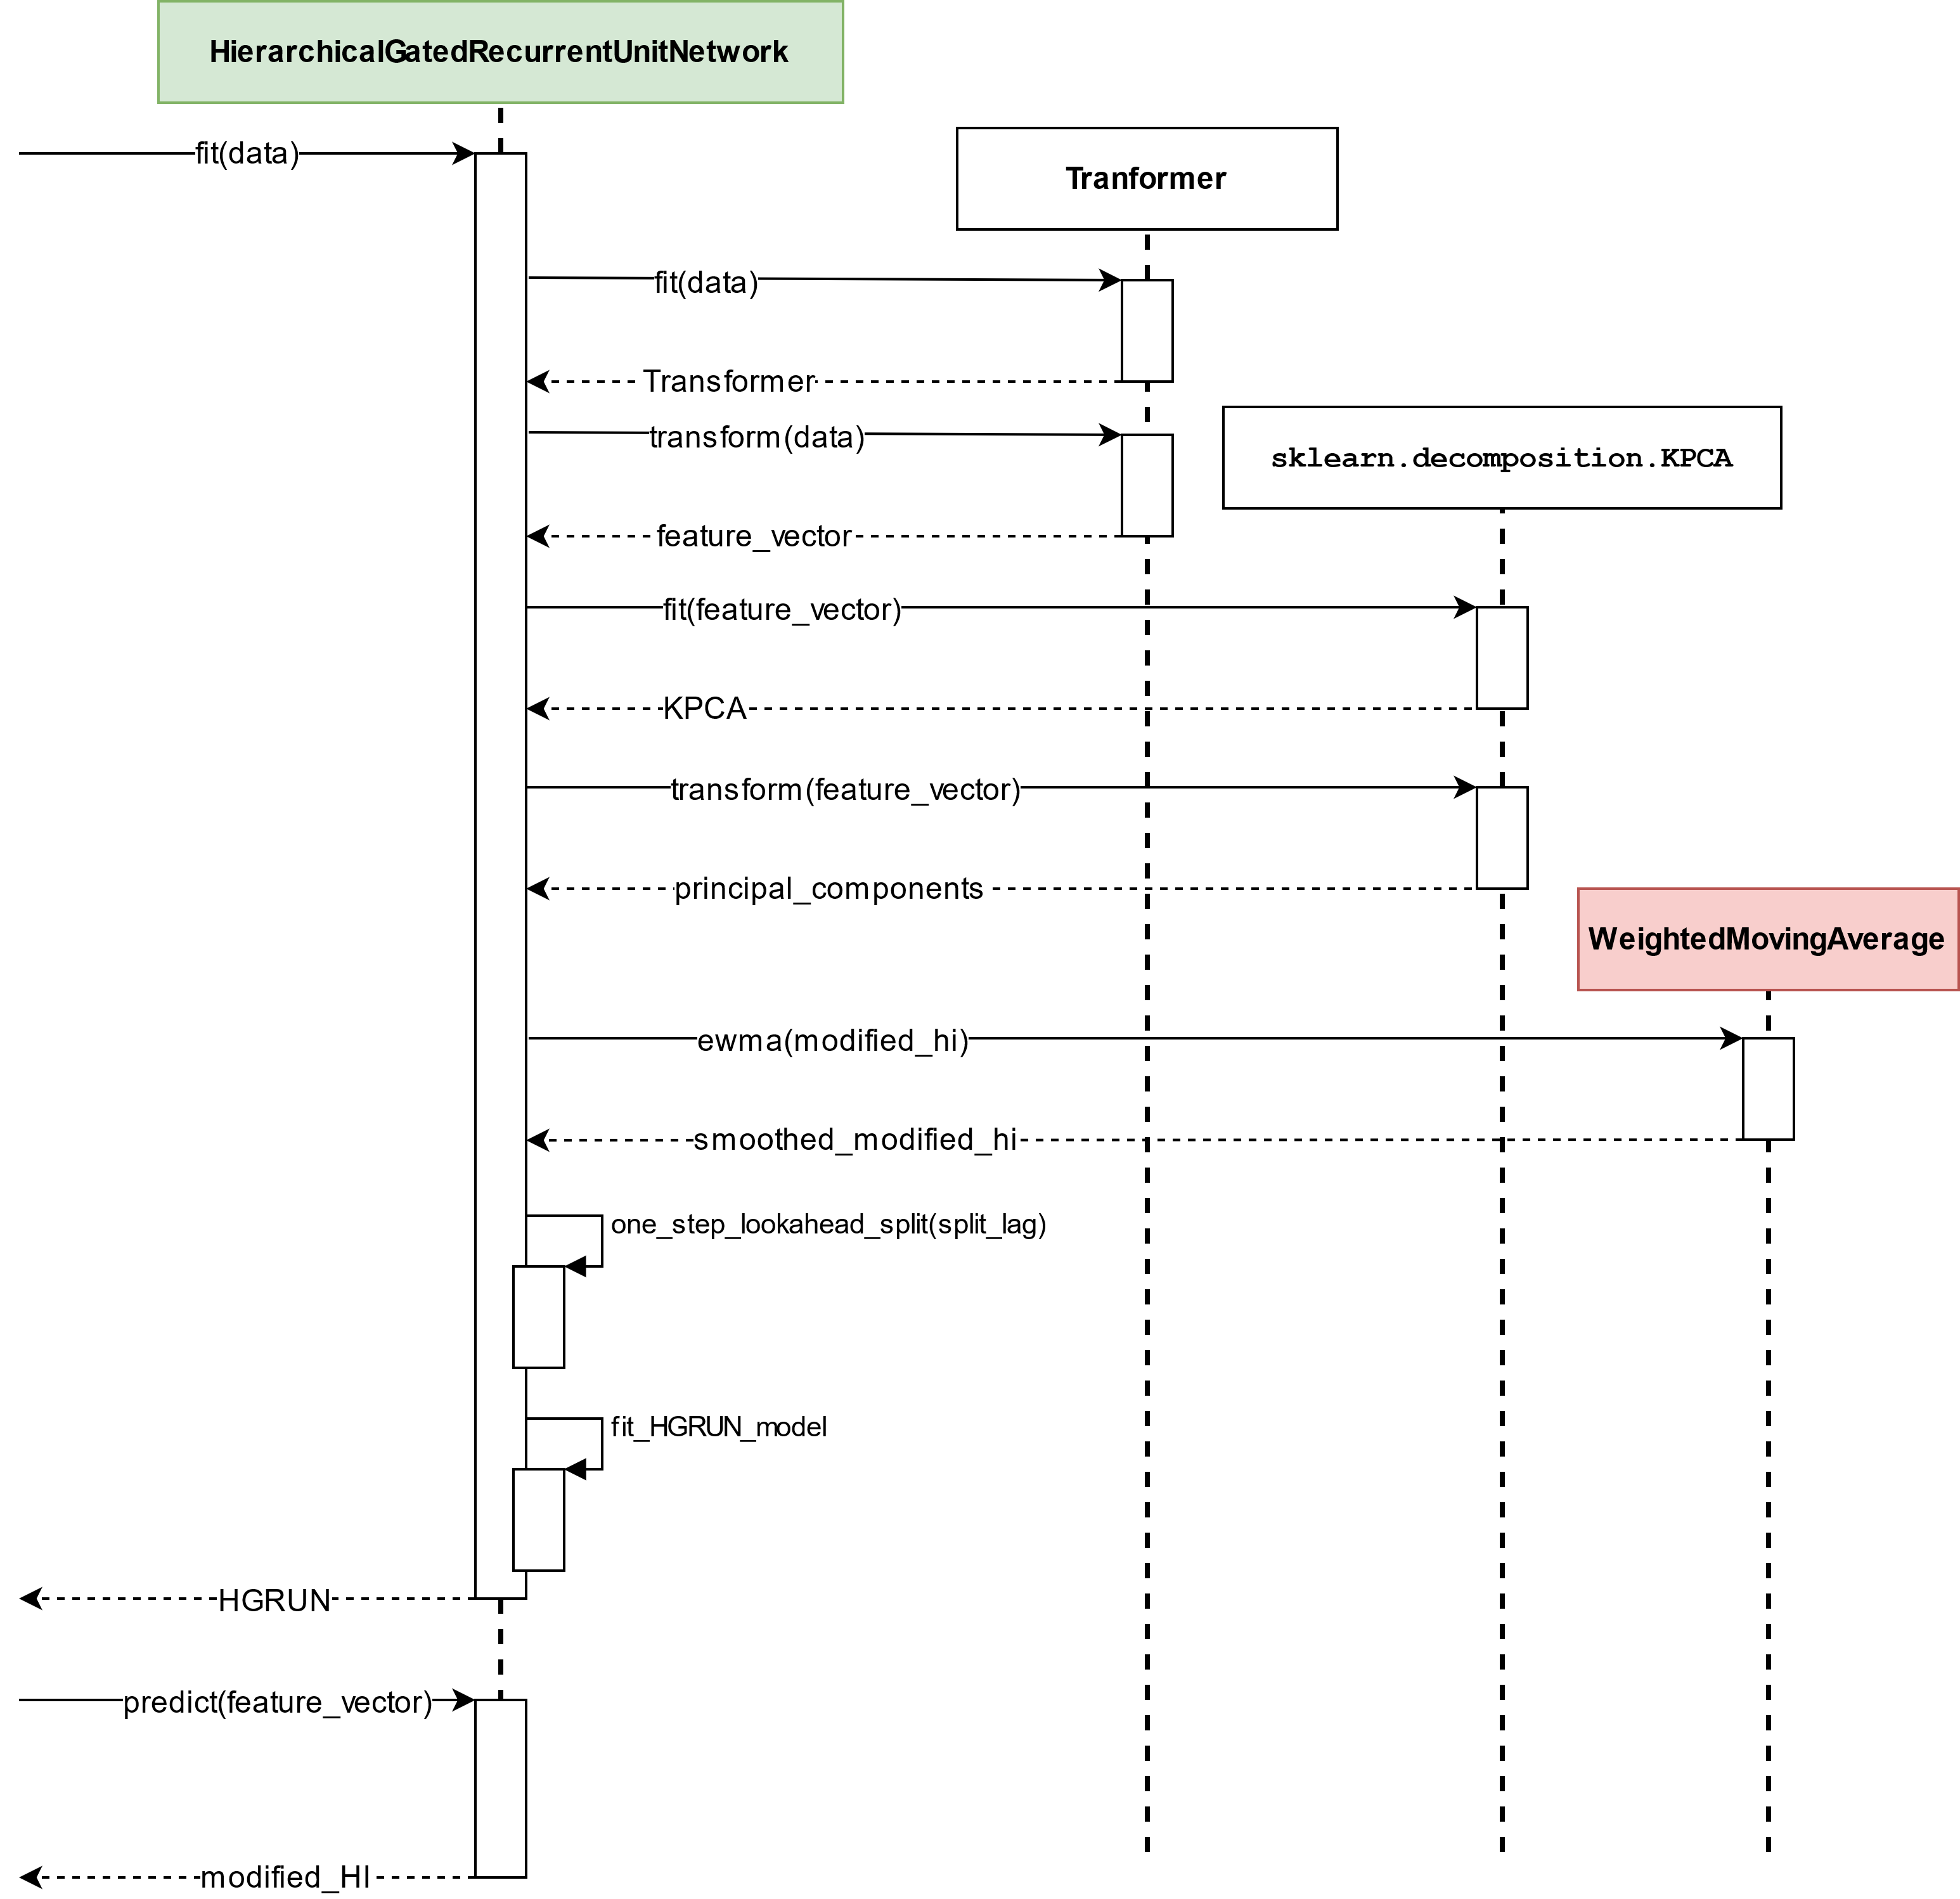
\includegraphics[width=\textwidth]{gfx/HGRUNsequencediagram.png}
    \caption{Hierarchical Gated Recurrent Unit Network HI estimation sequence diagram}
    \label{fig:sequence_hgrun}
\end{figure}

\begin{figure}[H]
    \centering
    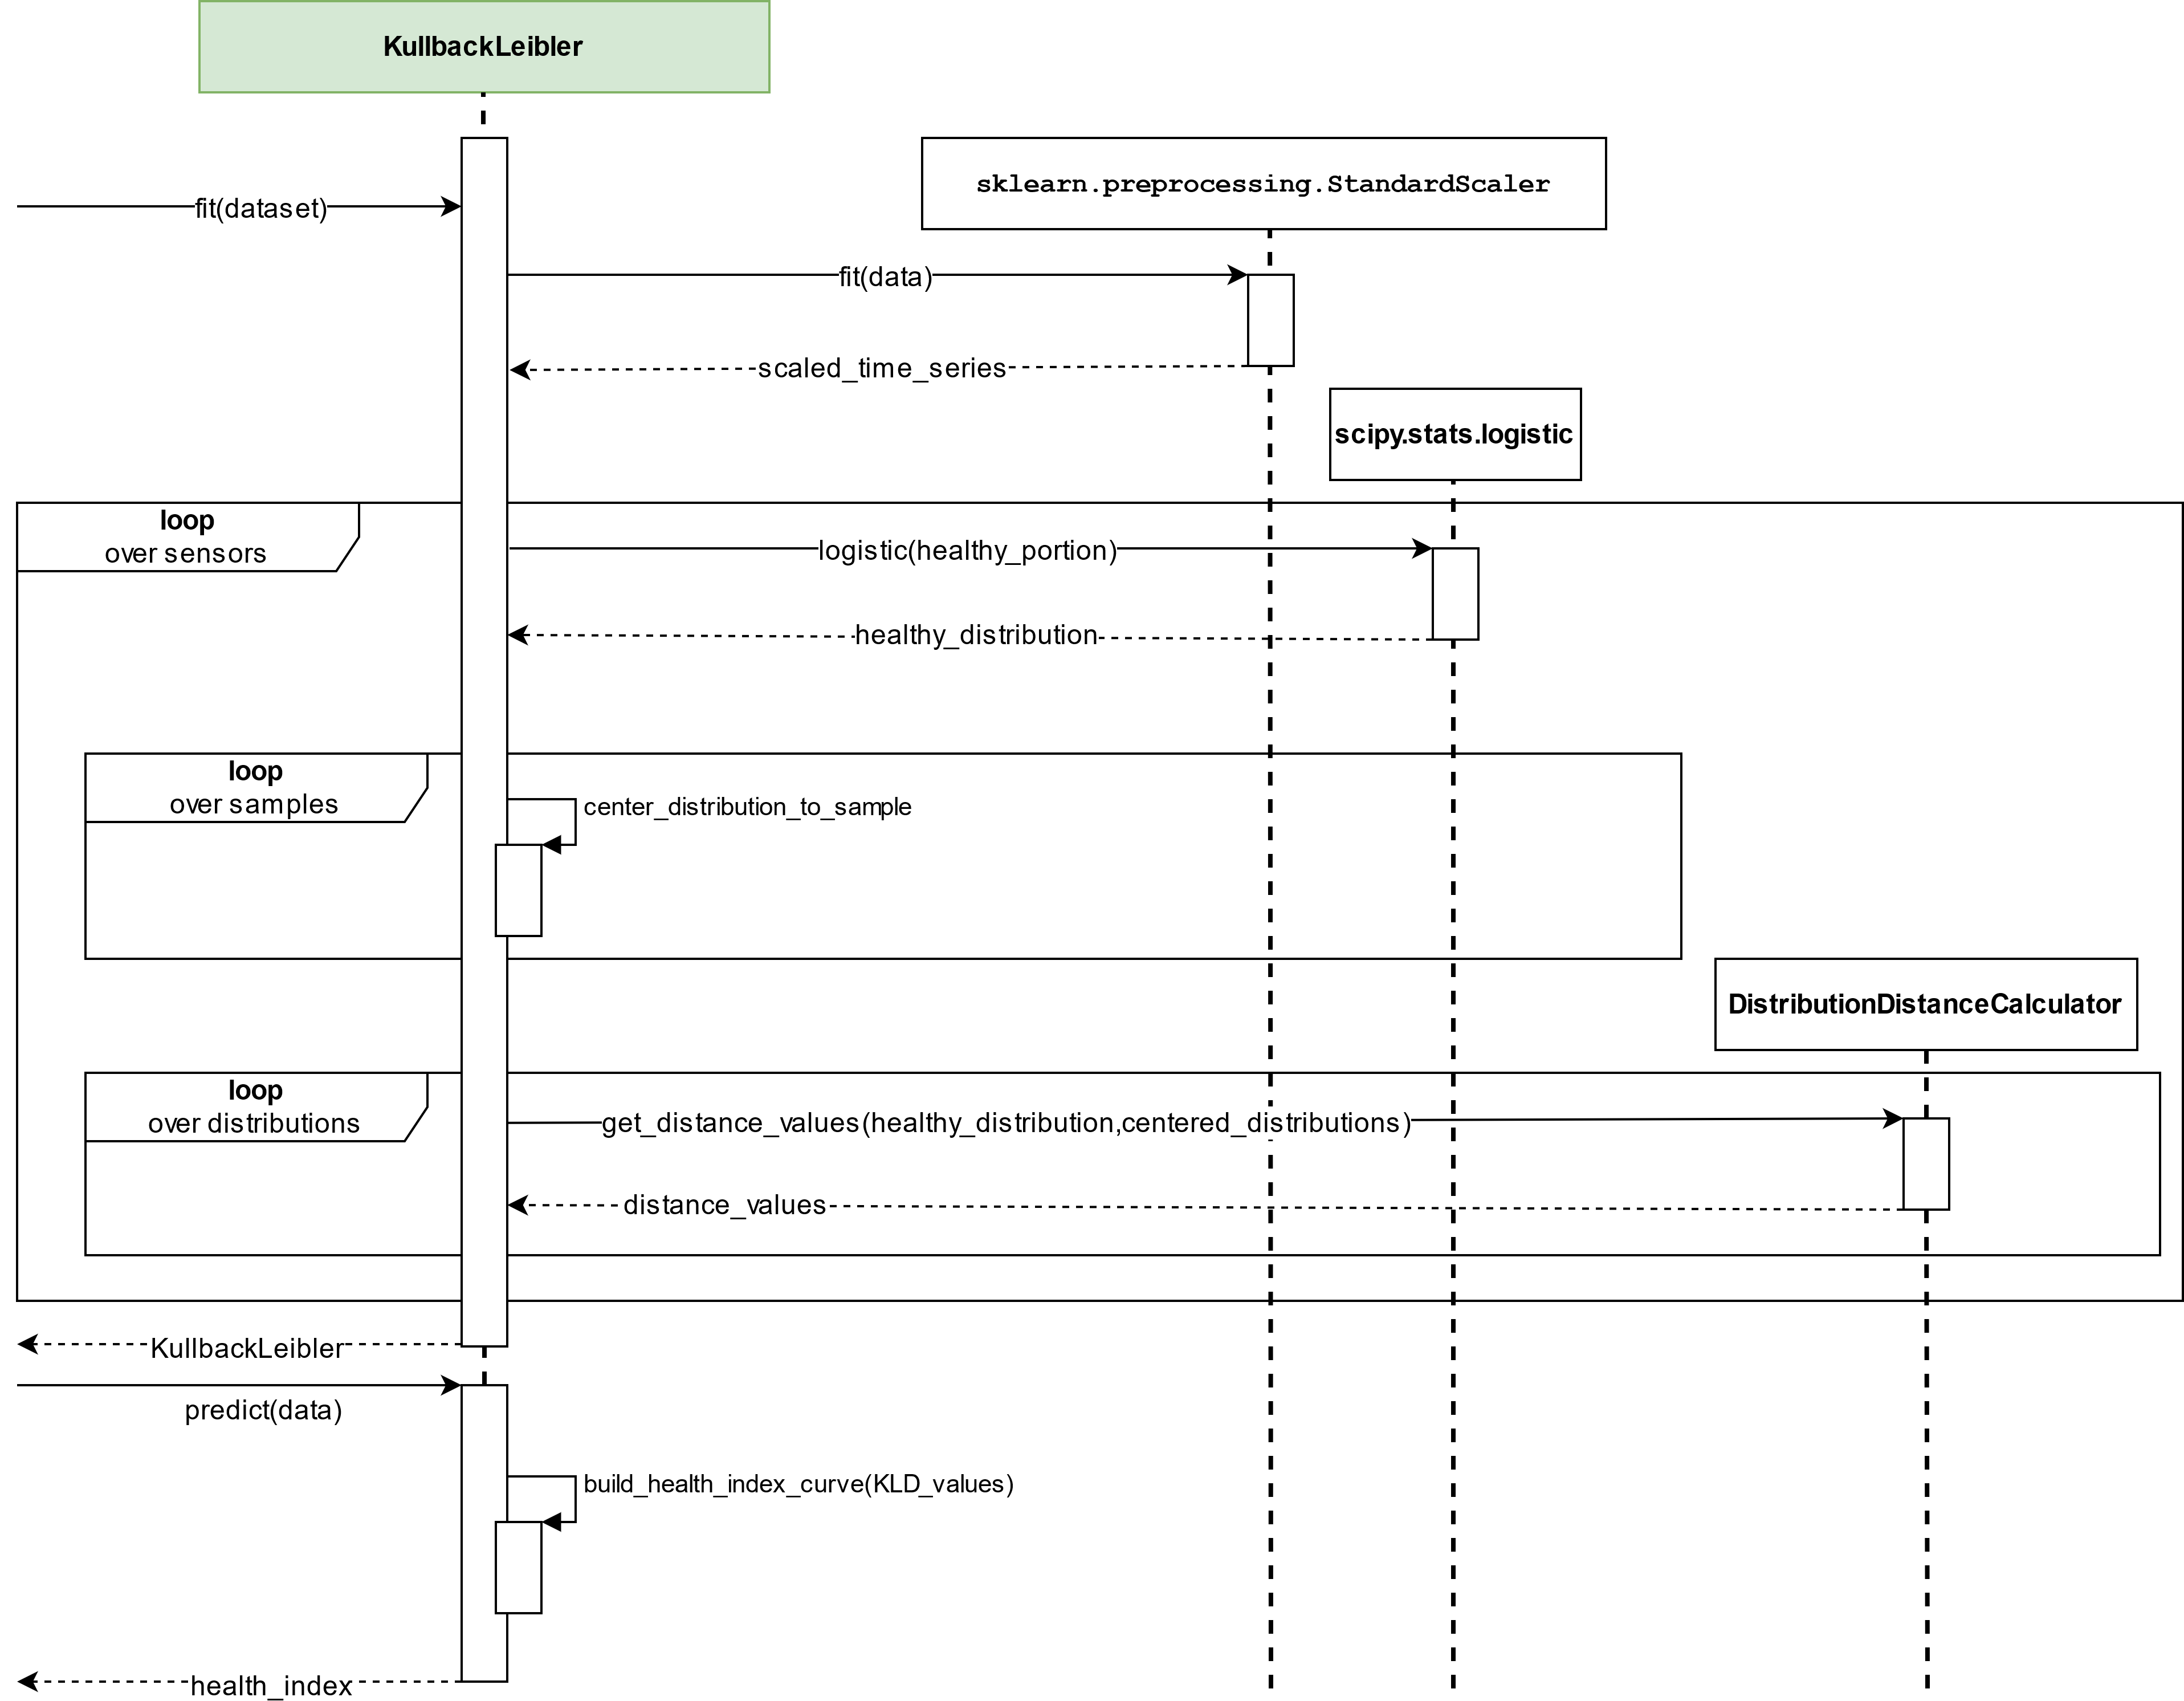
\includegraphics[width=\textwidth]{gfx/Kullbacksequencediagram.png}
    \caption{Kullback-Leibler Diveregence HI estimation sequence diagram}
    \label{fig:sequence_KLD}
\end{figure}

\section{Remaining Useful Lifetime Estimation}
\vspace*{-6.5mm}\hfill{\fontfamily{phv}\normalsize\emph{Vinay Kaundinya and Christopher Zinda}}

Different classes that are used in RUL estimation are described in this section, along with their parameters, methods and relationships.

\subsection*{Class diagram}
\vspace*{-12.5mm}\hfill{\fontfamily{phv}\normalsize\emph{Vinay Kaundinya and Christopher Zinda}}

The abstract class \textit{RemainingUsefulLifetimeEstimator} serves as a superclass for all RUL estimators and fixed pipelines. These will be described in an anti-clockwise manner in the following section.

The abstract class \textit{EnsembleApproach} in Figure \ref{fig:rul_class} acts as a superclass for all RUL approaches that consist of multiple elements of the same type. These elements are trained independently and when predicting the RUL, the individual predictions are aggregated to obtain a single prediction. One example of an ensemble approach is the \textit{MultipleClassifierApproach}. The \textit{MultipleClassifierApproach} saves the maximum failure horizon and holds multiple classifiers that are trained independently. The class \textit{EmbedRUL} resembles a pipeline out of four steps: \textit{WindowingApproach}, \textit{RNNAutoencoder}, \textit{HIEstimator}, \textit{RULEstimator}. Every pipeline step saves its configuration parameters that can also be set in the \textit{EmbedRUL} constructor. The \textit{transform} methods are specified to show the interconnection between the pipeline steps because the output of one step serves as an input to the next step. The abstract class \textit{CNN} in Figure \ref{fig:rul_class} acts as a superclass for all CNN approaches that allows user to choose only neural network model over the CNN approach that is proposed here. The abstract class \textit{SVR} then acts as a superclass for all SVR based approaches, which allows user to choose only SVR model over the Direct RUL approach which also extends an SVR model. The class \textit{LSTM} is nothing but a pipeline of calls to two normalizations \textit{MinMaxScaler} and \textit{StandardScaler} followed by different calls to methods in \textit{tf.keras.layers}.
\begin{figure}[H]
    \centering
    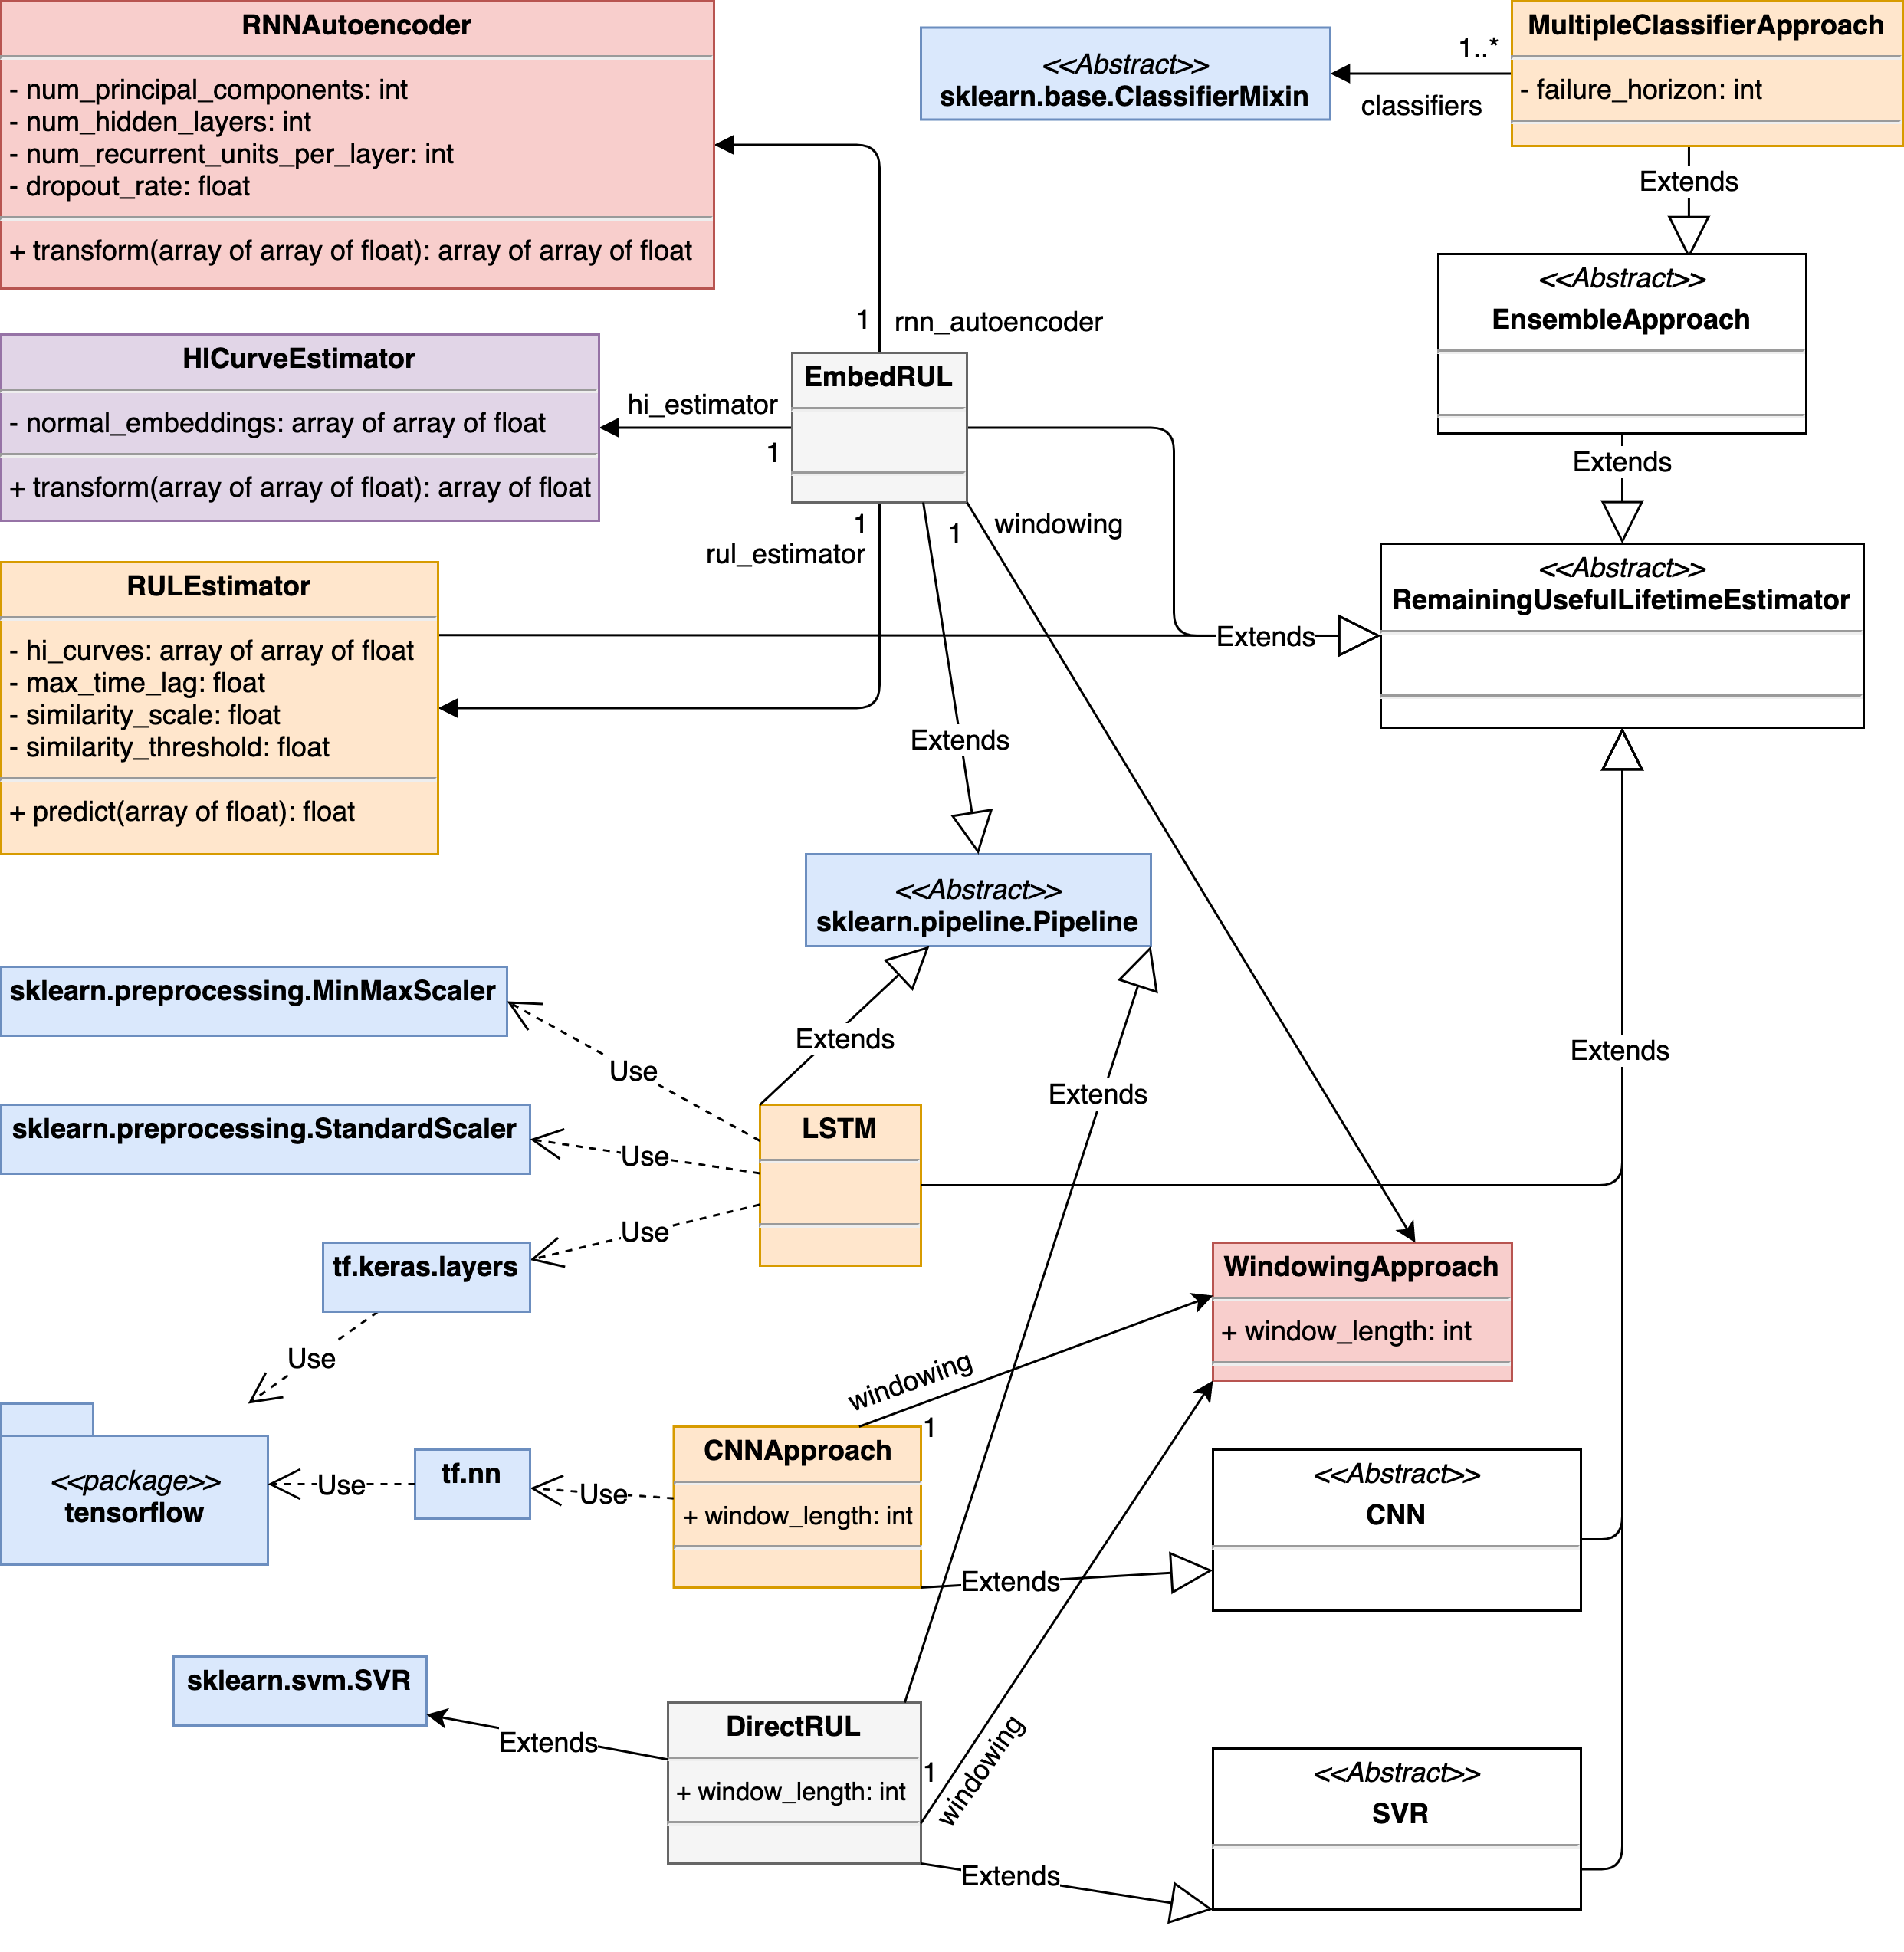
\includegraphics[width=\textwidth]{gfx/rul_class}
    \caption{Class diagram showing specific classes needed for Remaining Useful Lifetime Estimation.}
    \label{fig:rul_class}
\end{figure}

\subsection*{Sequence diagrams}
\vspace*{-12.5mm}\hfill{\fontfamily{phv}\normalsize\emph{Vinay Kaundinya and Christopher Zinda}}

Sequence diagrams for each of the RUL approaches are presented in the following section.

\subsubsection*{Multiple Classifier Approach}
\vspace*{-12.5mm}\hfill{\fontfamily{phv}\normalsize\emph{Christopher Zinda}}

The Multiple Classifier Approach is initialized with a parameter that defines the maximum failure horizon. As shown in Figure \ref{fig:rul_seq_multiple_classifier}, the array of \textit{ClassifierMixin} is initialized in the constructor. In the \textit{fit} method, the dataset is first prepared with annotations of different failure horizons. Every classifier is then fitted on one of the prepared datasets. In the \textit{predict} method we can then evaluate all classifiers and aggregate their predictions as described in the topic study document.
\begin{figure}[H]
    \centering
    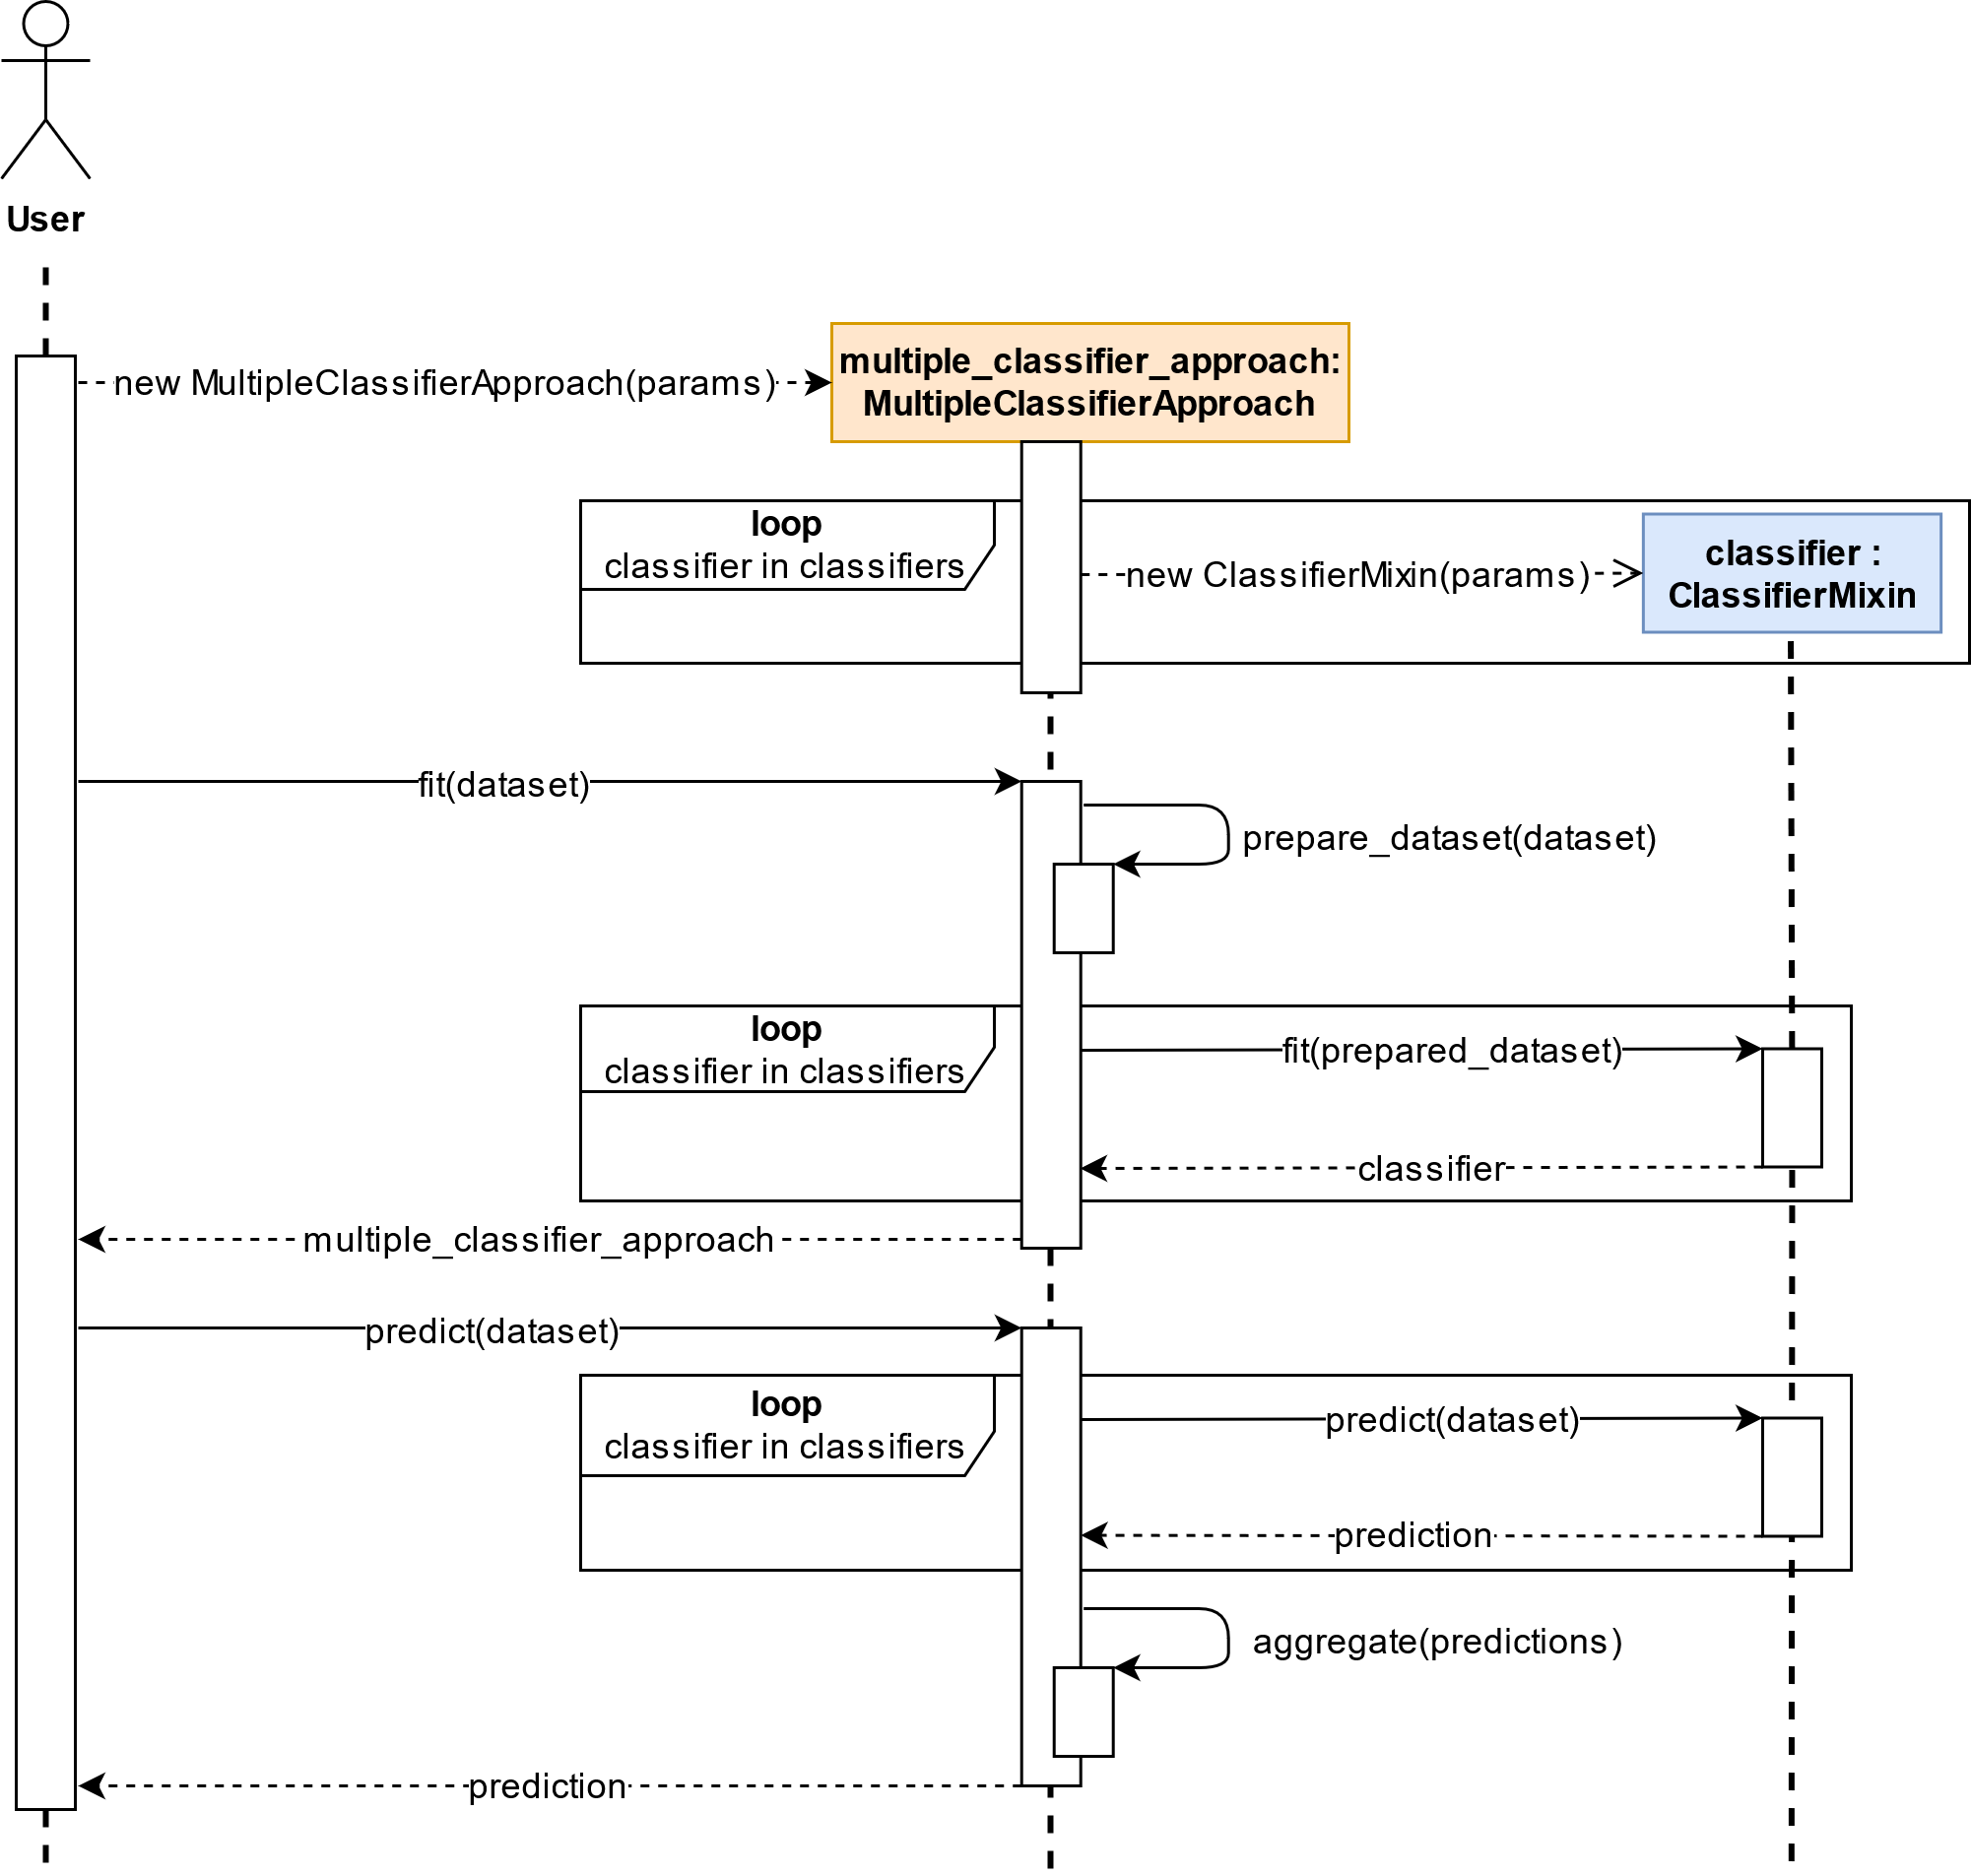
\includegraphics[width=\textwidth]{gfx/rul_seq_multiple_classifier}
    \caption{Sequence diagram of the Multiple Classifier Approach for fit and predict use case.}
    \label{fig:rul_seq_multiple_classifier}
\end{figure}

\subsubsection*{Embed RUL}
\vspace*{-12.5mm}\hfill{\fontfamily{phv}\normalsize\emph{Christopher Zinda}}

As shown in Figure \ref{fig:rul_seq_embed_rul}, the \textit{EmbedRUL} class first initializes the four pipeline steps \textit{WindowingApproach}, \textit{RNNAutoencoder}, \textit{HIEstimator} and \textit{RULEstimator}. These four elements are then also fitted in the same order. The output of one step is passed to the next step as input. The same pipeline execution happens in the \textit{predict} method to finally generate a RUL prediction. Details on the operation of each individual fit and transform/predict method can be found in the topic study document.
\begin{figure}[H]
    \centering
    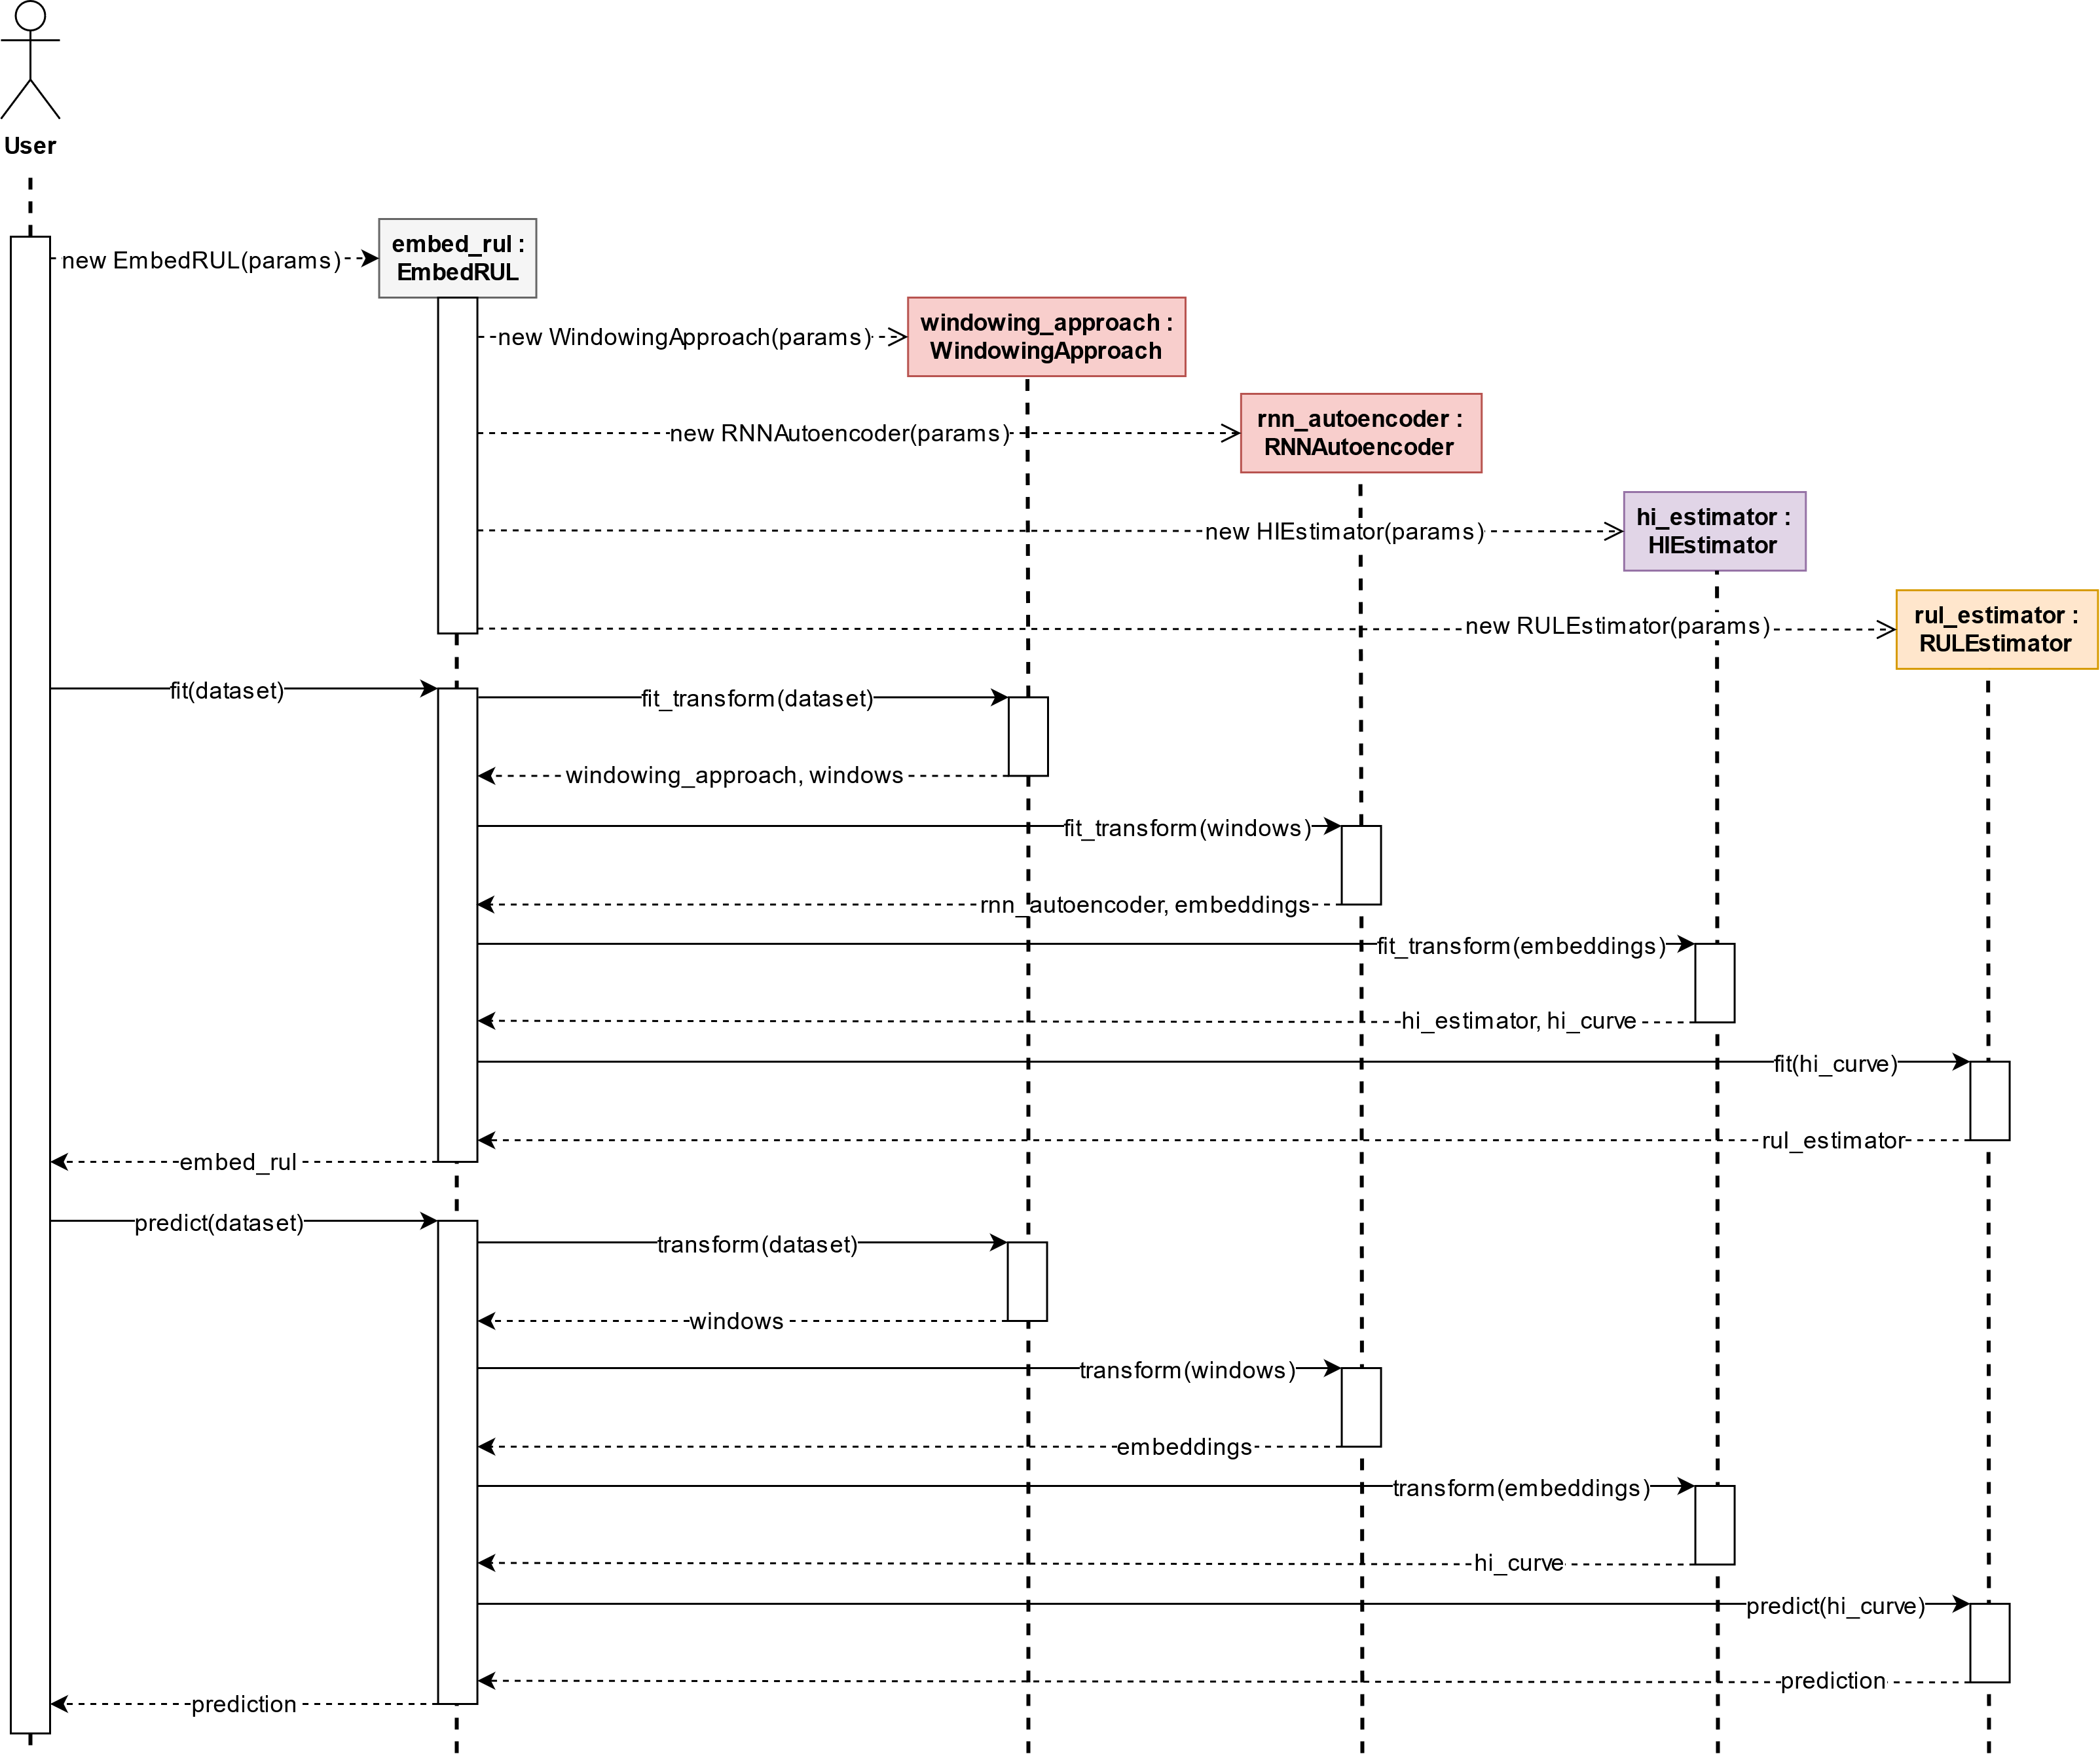
\includegraphics[width=\textwidth]{gfx/rul_seq_embed_rul}
    \caption{Sequence diagram of the Embed RUL class for fit and predict use case.}
    \label{fig:rul_seq_embed_rul}
\end{figure}

\subsubsection{Direct RUL}
\vspace*{-12.5mm}\hfill{\fontfamily{phv}\normalsize\emph{Vinay Kaundinya}}

Figure \ref{fig:rul_seq_direct_rul} shows how the \textit{DirectRUL} class first initializes \textit{WindowingApproach} and then initializes an \textit{SVR}, as a pipeline. The output of windowing approach is then passed to SVR as input. The same pipeline execution happens in both the \textit{fit} and \textit{predict} method to finally generate a RUL prediction.
\begin{figure}[H]
    \centering
    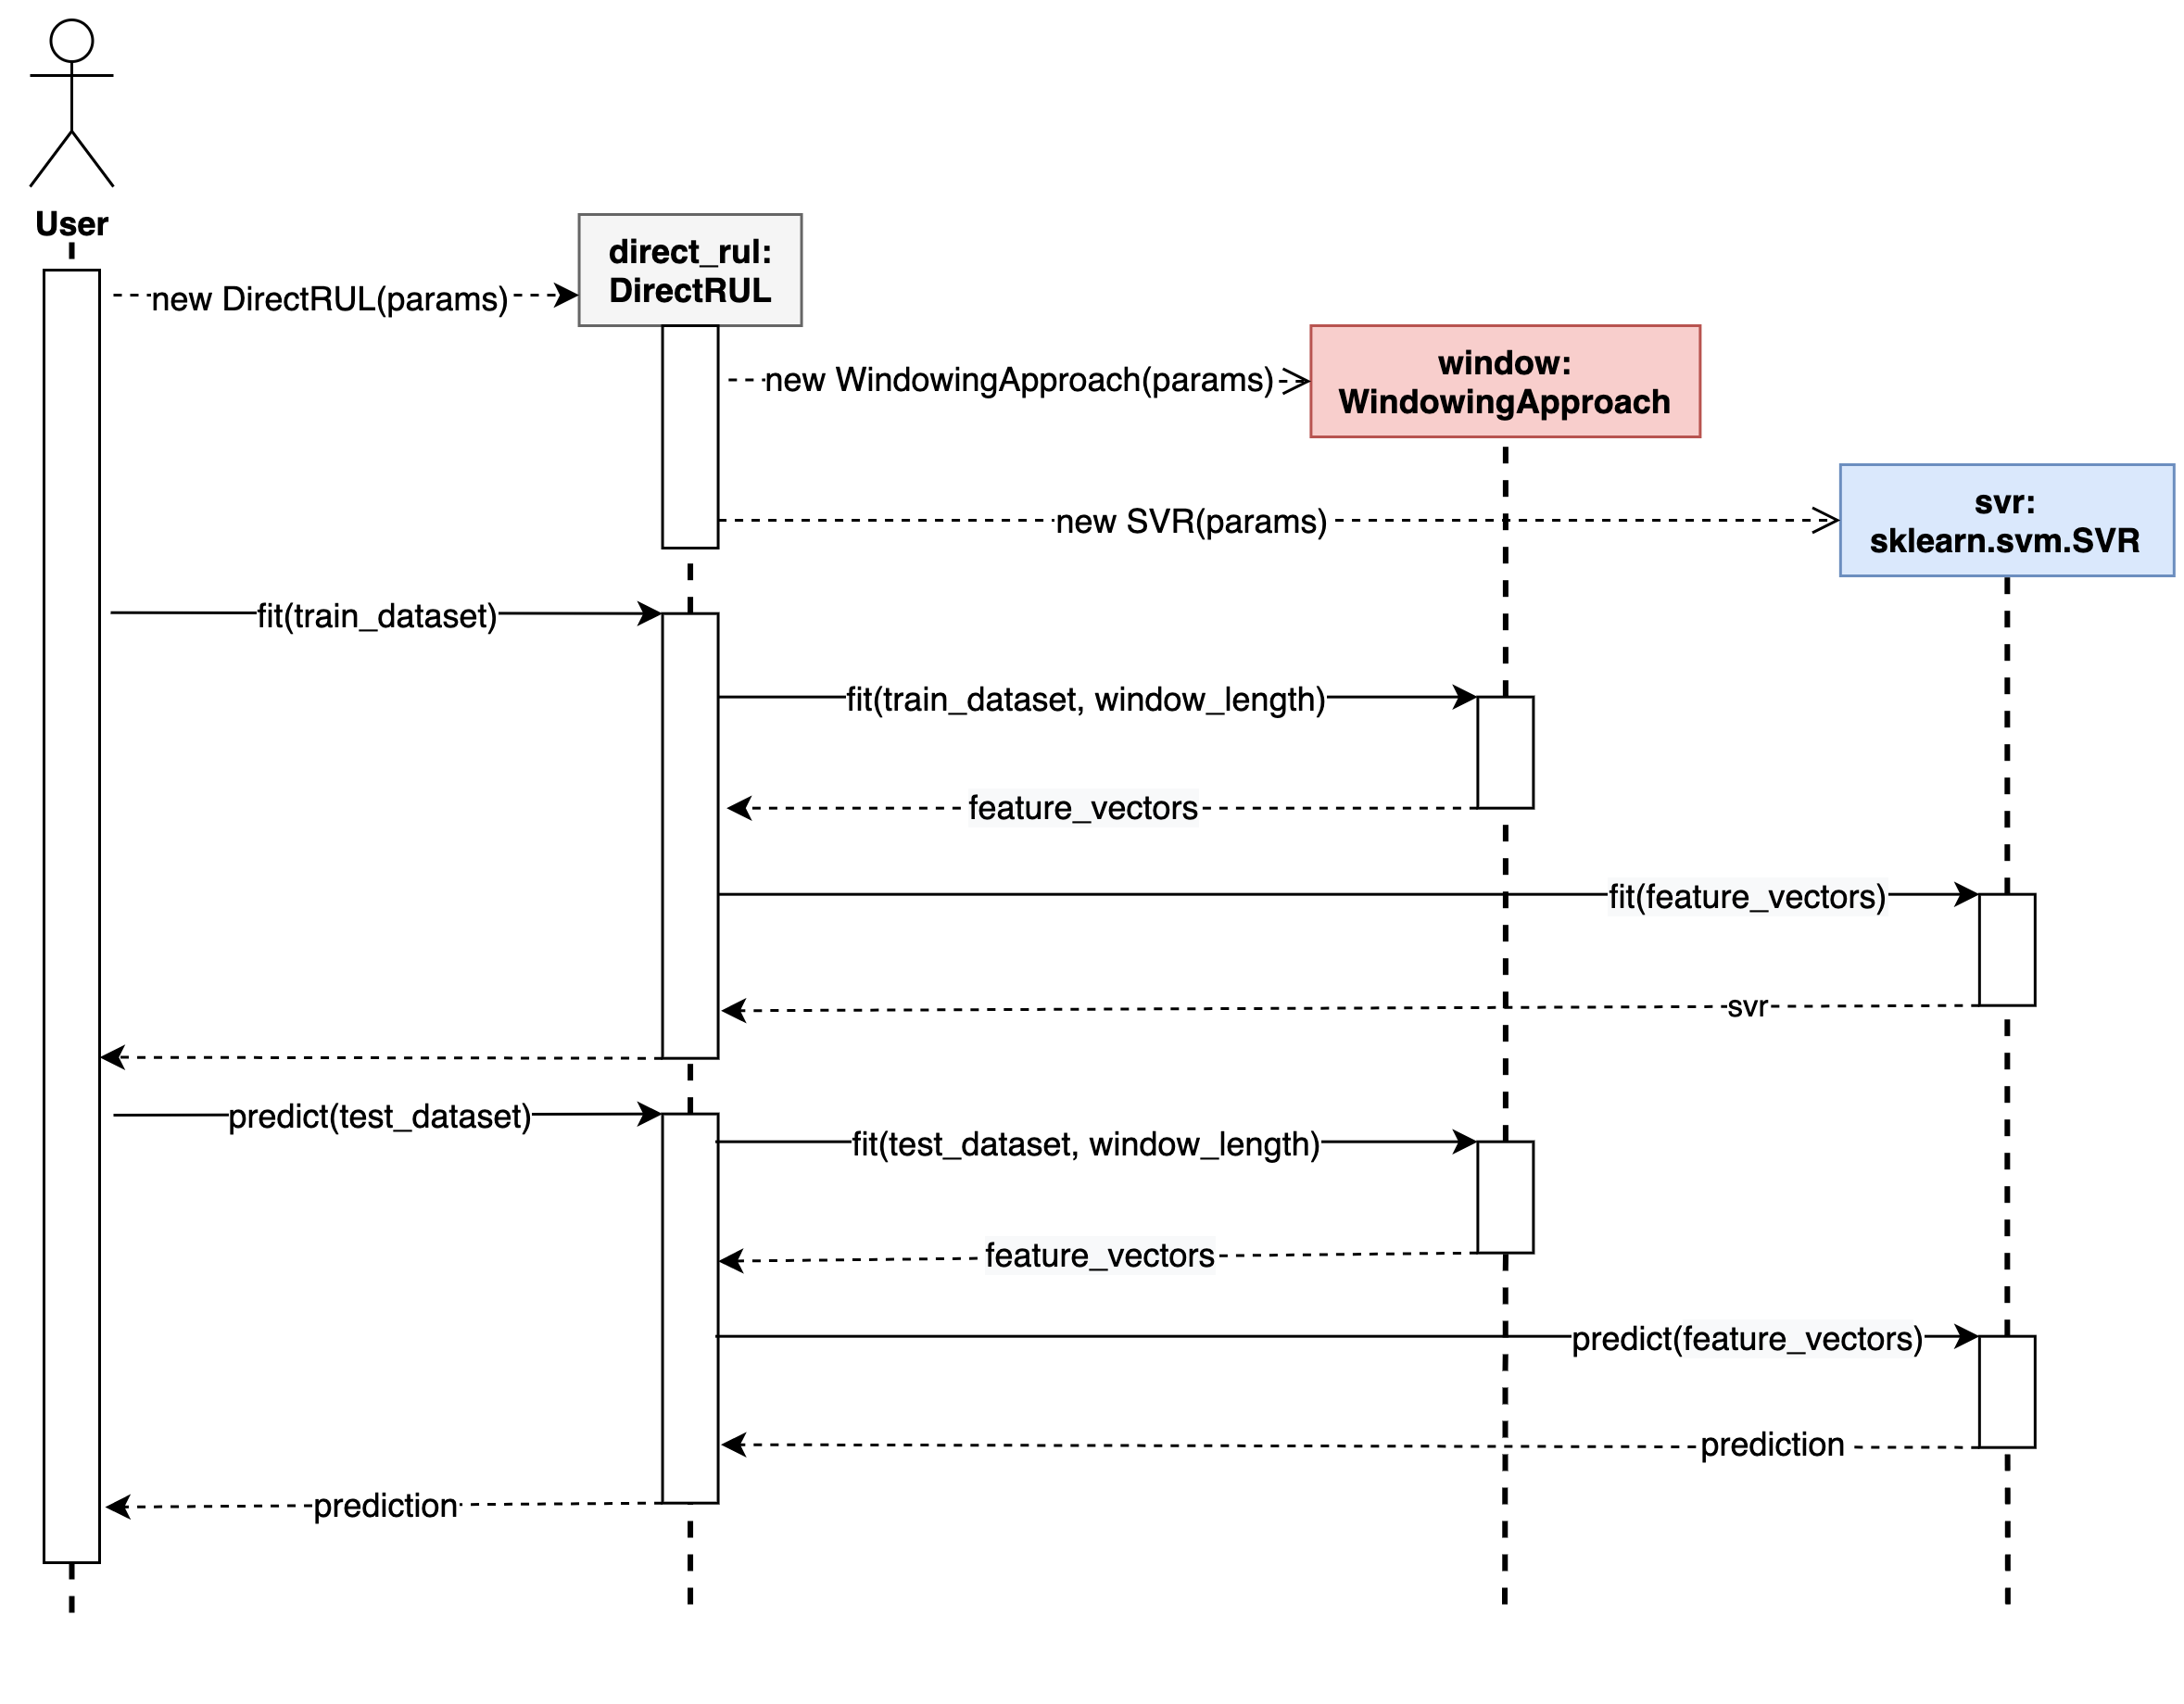
\includegraphics[width=\textwidth]{gfx/rul_seq_direct_rul}
    \caption{Sequence diagram of the direct RUL class for fit and predict use case.}
    \label{fig:rul_seq_direct_rul}
\end{figure}

\subsubsection{CNN}
\vspace*{-12.5mm}\hfill{\fontfamily{phv}\normalsize\emph{Vinay Kaundinya}}

Figure \ref{fig:rul_seq_cnn} shows how the \textit{CNN} class initializes \textit{WindowingApproach} and then initializes \textit{nn}(neural network module), as a pipeline. The output of windowing approach is then passed to neural network as input. The same pipeline execution happens in both the \textit{fit} and \textit{predict} method to finally generate a RUL prediction.
\begin{figure}[H]
    \centering
    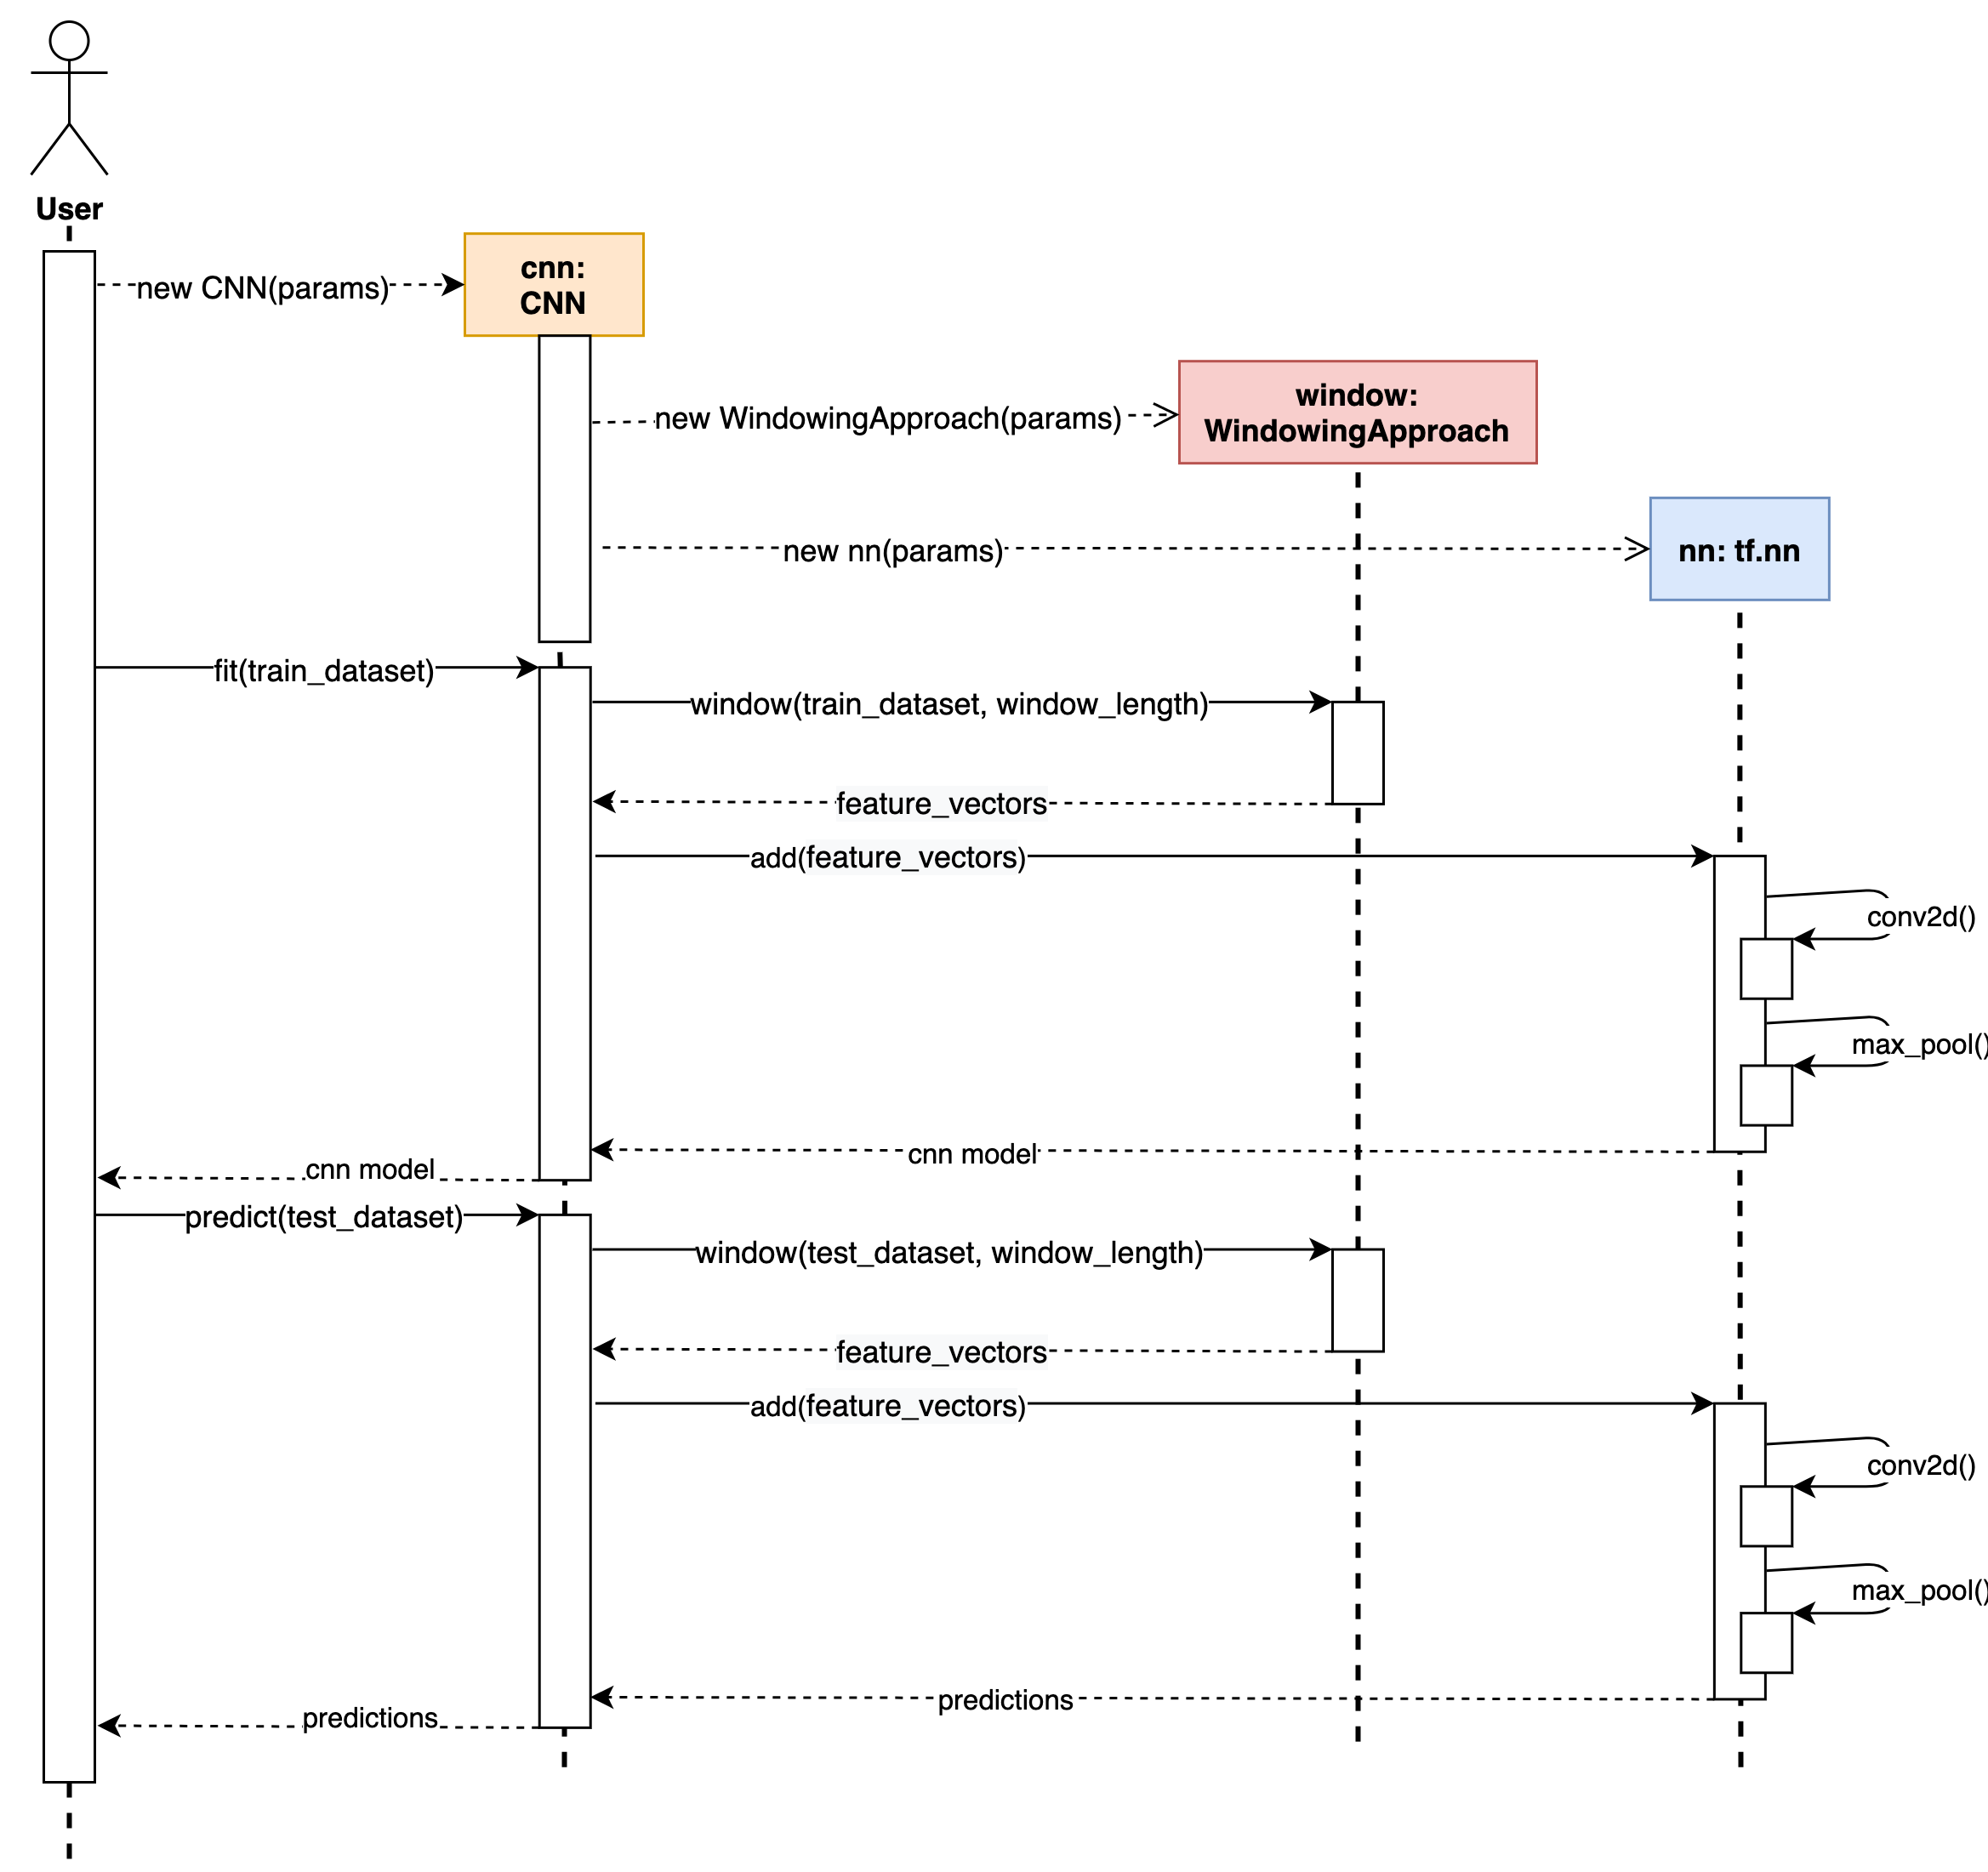
\includegraphics[width=\textwidth]{gfx/rul_seq_cnn}
    \caption{Sequence diagram of the CNN class for fit and predict use case.}
    \label{fig:rul_seq_cnn}
\end{figure}

\subsubsection{LSTM Approach}
\vspace*{-12.5mm}\hfill{\fontfamily{phv}\normalsize\emph{Vinay Kaundinya}}

In the figure \ref{fig:rul_seq_lstm}, \textit{LSTM} class initializes \textit{MinMaxScaler}, \textit{StandardScaler} and then initializes an instance of \textit{tf.keras.layers}. It shows that the dataset is passed through the two scalers before passing them into layers of LSTM.
\begin{figure}[H]
    \centering
    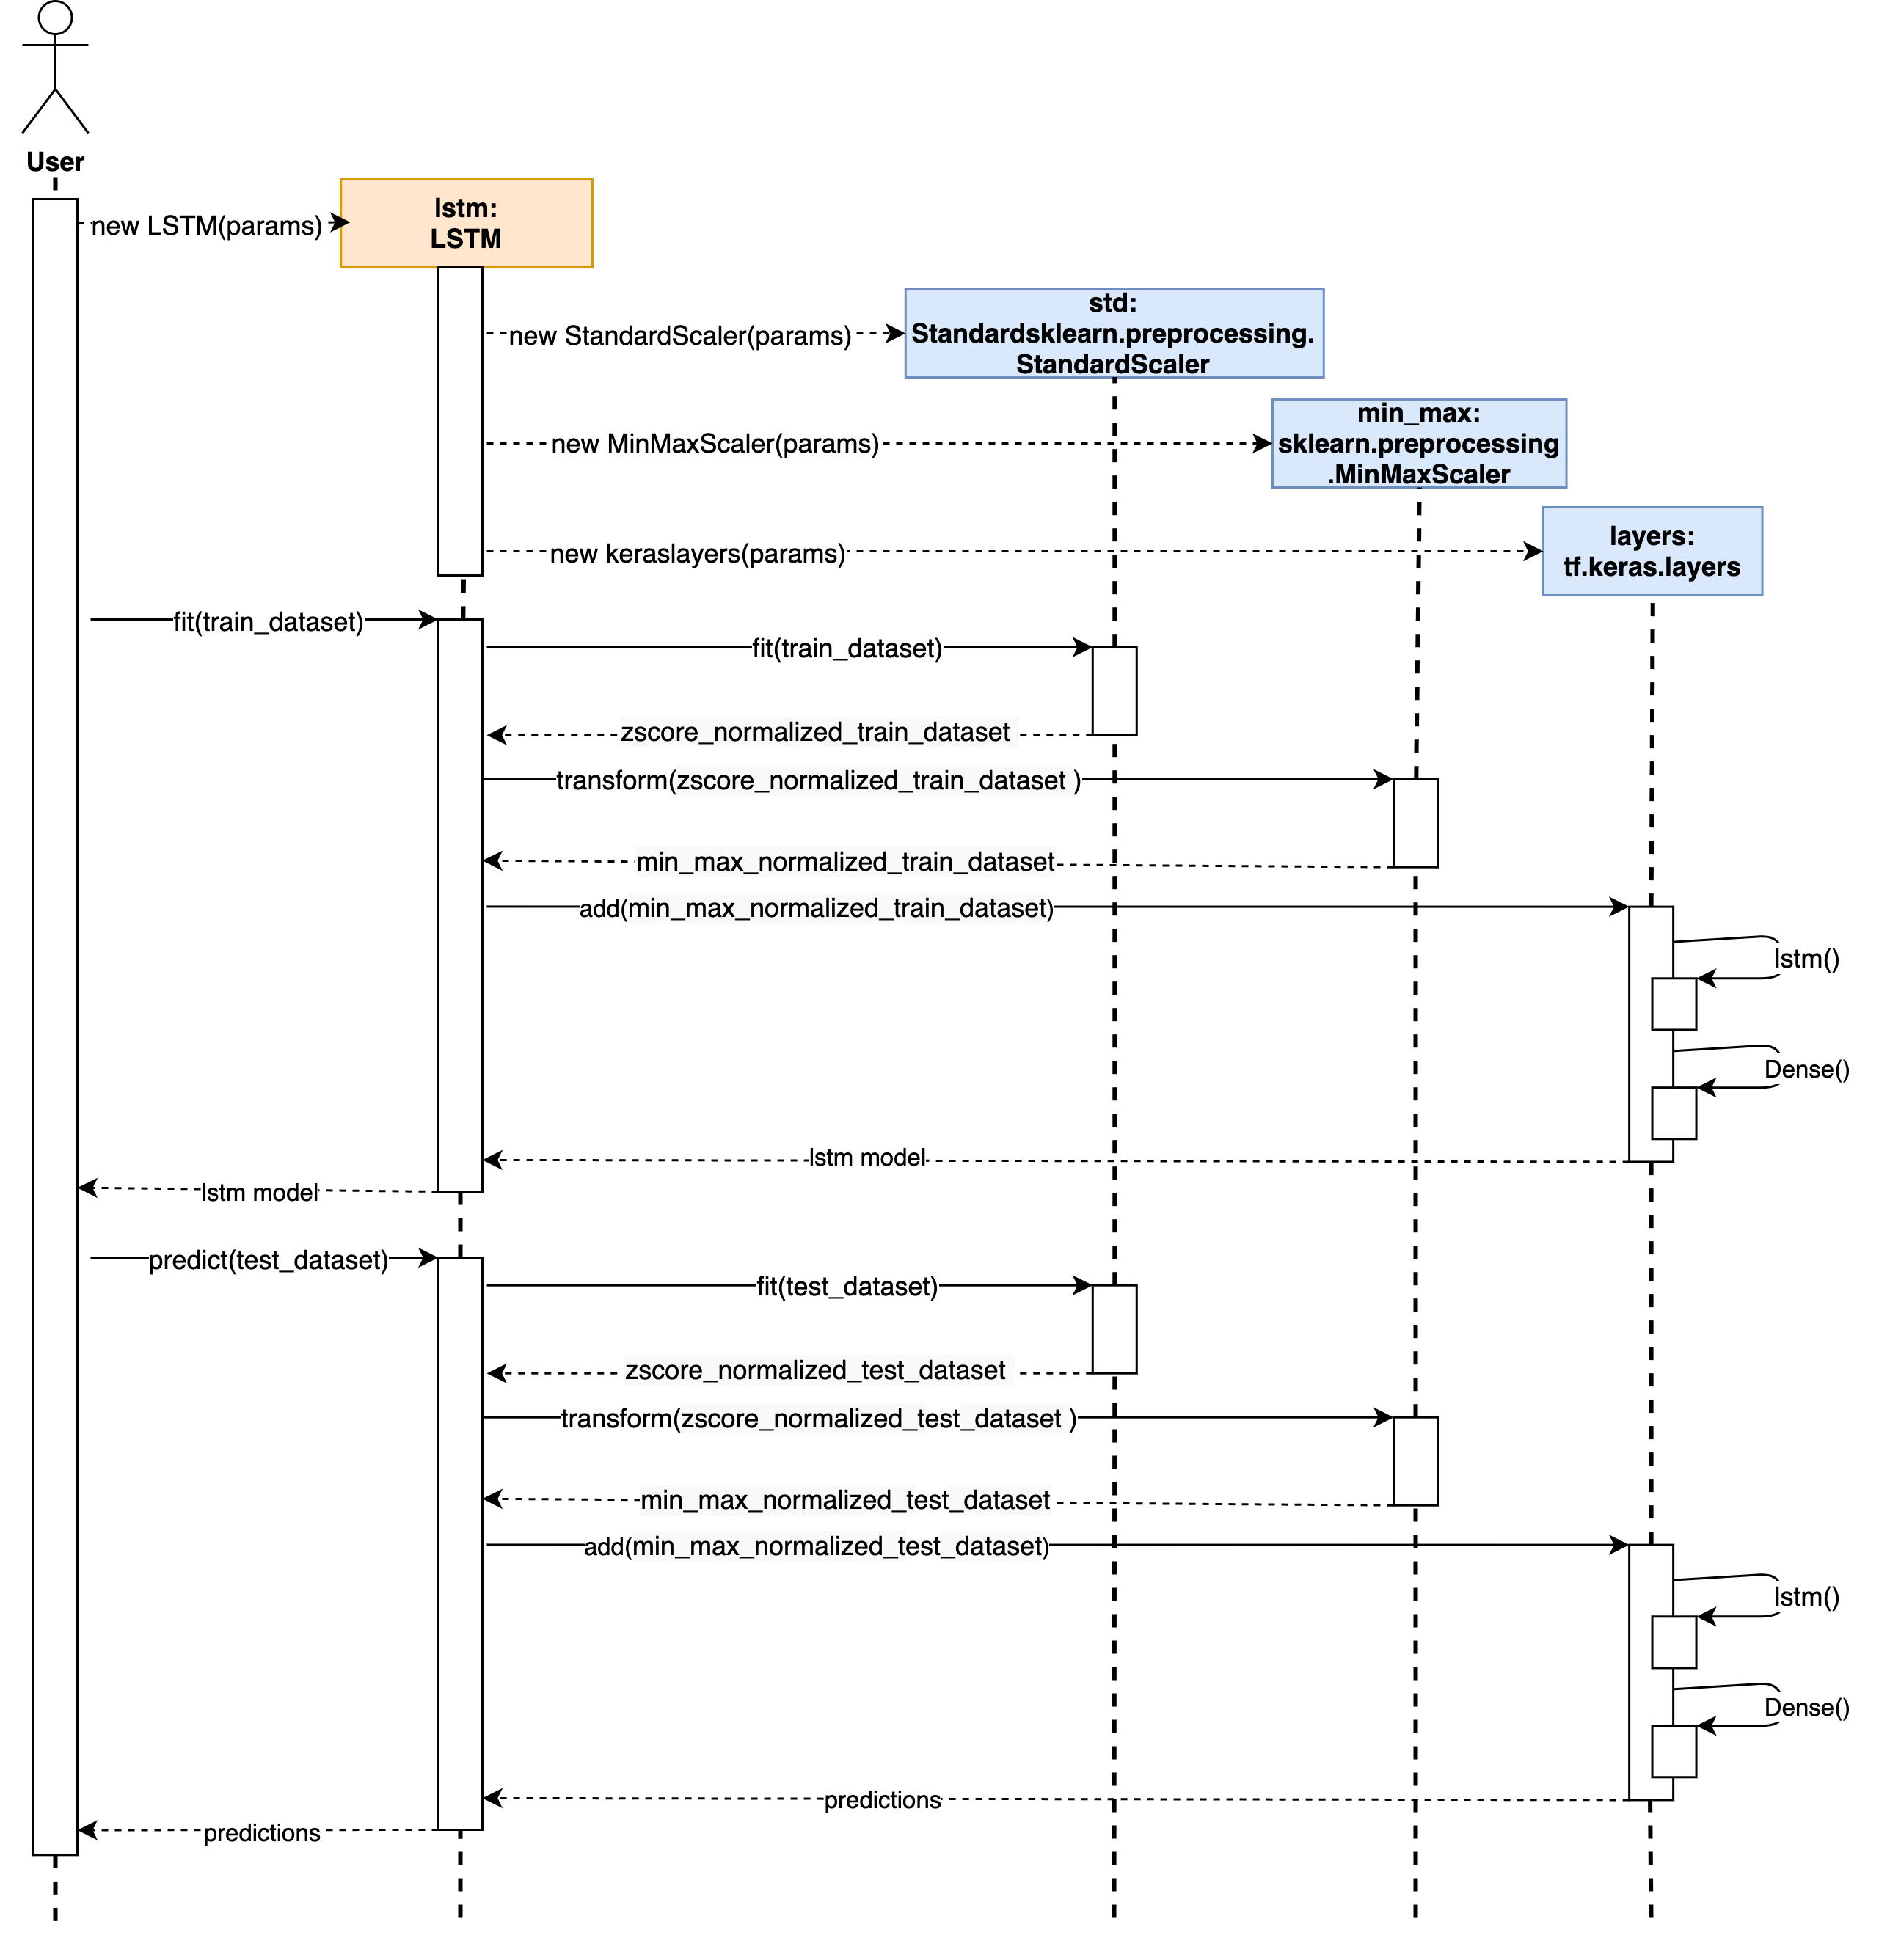
\includegraphics[width=\textwidth]{gfx/rul_seq_lstm}
    \caption{Sequence diagram of the LSTM class for fit and predict use case.}
    \label{fig:rul_seq_lstm}
\end{figure}           % INCLUDE: system-design
% !TEX root = ../main_sys.tex
%
\chapter{Quality Assurance}
\label{sec:quality_assurance}

In this chapter we describe our continuous integration pipeline, the testing strategy, our git strategy and our documentation strategy that are used during development of the ML4PdM library.

\section{Continuous Integration}
\vspace*{-10mm}\hfill{\fontfamily{phv}\normalsize\emph{Christopher Zinda}}
\label{sec:quality_assurance:ci}

For continuous integration while developing the ML4PdM library, the GitLab CI/CD pipeline is used. It is executed on every commit to the master and develop branches as well as merge requests and tags. This ensures a sufficient quality control while limiting the number of failed pipelines by not including feature branches.

The CI/CD pipeline contains two jobs which are running in parallel. One job submits the changes to the SonarQube\footnote{\href{https://www.sonarqube.org/}{https://www.sonarqube.org/}} which is a self-hosted version of the SonarCloud\footnote{\href{https://sonarcloud.io/}{https://sonarcloud.io/}}. It will detect bugs, vulnerabilities, code smells, failed tests and test coverage in an automated manner. The results are displayed on a detailed dashboard for manual analysis by the developers. The second job will use the Sphinx\footnote{\href{https://www.sphinx-doc.org/en/master/index.html}{https://www.sphinx-doc.org/en/master/index.html}} Python documentation generator to automatically generate a static HTML page as well as a PDF document containing the class documentation and usage examples. The documentation is described in detail in section \ref{sec:quality_assurance:doc}.

A failed pipeline execution has to be fixed by the author of the changes. Merges to the master branch are not allowed until all errors have been corrected and the pipeline runs without errors. This will always ensure a tested and working code base on the master branch.
\newpage
\section{Testing Strategy}
\vspace*{-10mm}\hfill{\fontfamily{phv}\normalsize\emph{Paul Fährmann}}
\label{sec:quality_assurance:testing}

We will use \textit{pytest}\footnote{\href{https://docs.pytest.org/en/stable/}{https://docs.pytest.org/en/stable/}} for our automated tests. We will try to automate all our tests, but we probably will have tests that are more sophisticated and it's unsure if they can be automated. We can identify three levels of testing which are progressively harder to test automatically:
\begin{enumerate}
	\item Unit Test\\
	      We test individual functions and classes.
	      \begin{itemize}
		      \item Testing all parser classes and their configuration classes as well as the DataSet class.\\
		            Testing some example configuration files, in wrong and correct format. Also using different sensor data types and testing the functionality of \verb|@Target| in our data format.
		      \item Testing every pipeline element class.\\
		            Checking that the input and output format types are correct and also that the classes calculate what they should calculate according to our topic study and system design document.
		      \item Testing the Evaluator\\
		            Checking that the evaluator correctly loops through all the components and that it aggregates the resulting scores/losses correctly.
		      \item Testing the metrics\\
		            Testing that the metrics calculate the correct values.
	      \end{itemize}
	\item Integration Test\\
	      Testing that our predictor/transformer classes can work together with the sklearn classes in make\_pipeline and make\_union as well as other ways of integrating \verb|sklearn| and \verb|ml4pdm|.
	\item System Test\\
	      For three different knowledge-levels of users (beginner, intermediate, professional) we have tests of our system.
	      \begin{enumerate}
		      \item[1)] Beginner level: check that our library/evaluator can be used easily via the command line and get out error/score values and an actual model.
		      \item[2)] Intermediate level: check that a small part of predefined pipeline can be changed easily.
		      \item[3)] Professional level: check that each component of our library can be accessed and used individually without changing anything in the library itself.
	      \end{enumerate}
\end{enumerate}

\section{Documentation Strategy}
\vspace*{-10mm}\hfill{\fontfamily{phv}\normalsize\emph{Vinay Kaundinya}}
\label{sec:quality_assurance:doc}

Here we present a wholesome strategy for documenting code in describing its use and functionality to users, that is applied in the development of ML4PdM approaches. The idea is to keep it concise enough to be easy to maintain but still be elaborate enough for users to understand how to use the documented code.

\subsection{Documenting Code}
We use \textit{Docstrings} in documenting our code. Docstrings are built-in strings when configured correctly can help in documenting library's functionality for its users.

Docstrings have documentation of code written within triple-double($"""$) quotes.
\begin{figure}[H]
	\centering
	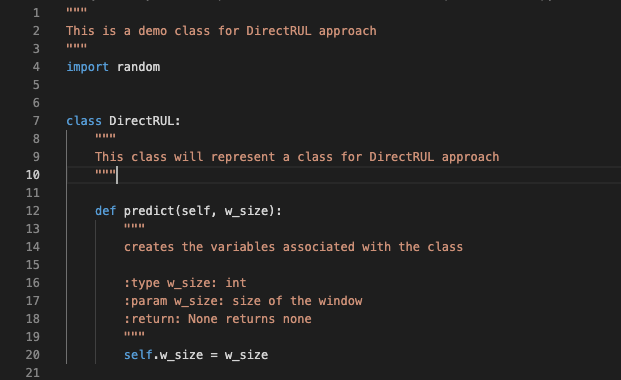
\includegraphics[width=10cm,height=6cm]{gfx/ex_docstring.png}
	\caption{Docstrings used in demo code describing a classes and its methods and parameters.}
	\label{fig:docstring}
\end{figure}
Docstrings are created for classes, as well as any class methods. The docstrings are placed immediately following the class or class method declaration. A docstring for a class should contain the following mandatory points,
\begin{itemize}
	\item A brief summary of its purpose and behavior.
	\item Any public methods, along with a brief description.
	\item Any class attributes.
\end{itemize}
An example of the same is also shown in the figure \ref{fig:docstring}.

\subsection{Document Generation}

We use Sphinx to generate documentation from docstrings in the python scripts of the project. Sphinx can provide documentation output in HTML, LaTeX (for printable PDF versions), ePub, Texinfo, manual pages, plain text formats. Sphinx uses reStructuredText as its markup language, and many of its strengths come from the power and straightforwardness of reStructuredText.

A reStructuredText document is made up of body or block-level elements, and may be structured into sections. Sections are indicated through title style (underlines and optional overlines). Sections contain body elements and/or subsections. Some body elements contain further elements, such as lists containing list items, which in turn may contain paragraphs and other body elements. Others, such as paragraphs, contain text.

Sections are identified through their titles, which are marked up with adornment: "underlines" below the title text, or underlines and matching "overlines" above the title.
Below are examples of section title styles:\begin{verbatim}
===============
 Section Title
===============

---------------
Section Title
---------------

Section Title
=============

Section Title
-------------

Section Title
`````````````

Section Title
*************

Section Title
+++++++++++++\end{verbatim}
\begin{figure}[H]
	\centering
	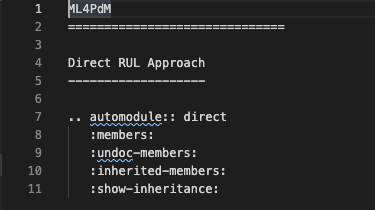
\includegraphics[width = 6cm]{gfx/ex_rst.png}
	\captionsetup{justification=centering}
	\caption{Example of reStructuredText document.}
	\label{fig:rst}
\end{figure}
In our document we use \textit{sphinx\_rtd\_theme} theme and this is configured while installing the sphinx document generator.
The documentation is then structured into following sections:
\begin{itemize}
	\item \textbf{Installation}: In this section we describe ways to invoke this library and all the other installation details.
	\item \textbf{Examples}: Here we list some examples of how the ML4PdM library can be used.
	\item \textbf{ML4PdM}: All the ML4PdM approaches, along with their classes, methods and parameters are documented under this section.
	\item \textbf{Release}: This section lists all the releases.
	\item \textbf{Glossary}: This section consists of keyword definitions used in documenting the approaches.
	\item \textbf{References}: Lists all the references to scientific papers, websites, books and datasets.
\end{itemize}
\begin{figure}[H]
	\centering
	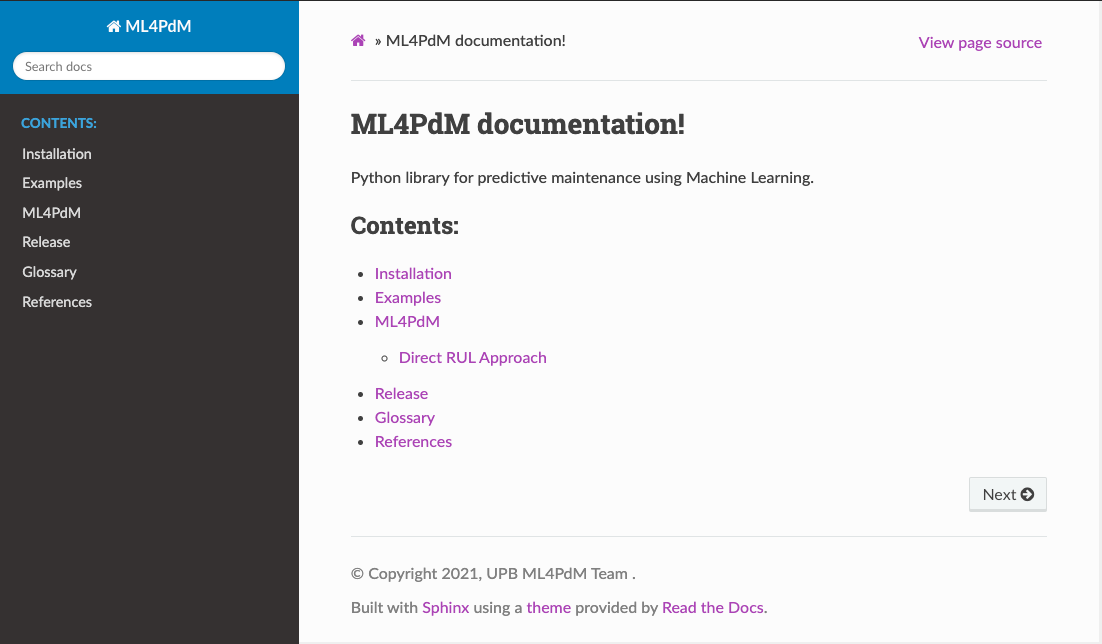
\includegraphics[width=12cm,height=6cm]{gfx/html.png}
	\caption{Example of HTML output of sphinx document generator for the planned sections.}
	\label{fig:html_output}
\end{figure}

\section{Git Strategy}
\vspace*{-10mm}\hfill{\fontfamily{phv}\normalsize\emph{Sanjay Gupta}}
\label{sec:quality_assurance:git}

In this section, we set the guidelines for the Git commit messages, versioning, Git structure, and branch merge. Git is a free and open-source distributed version control system that manages a project of any size. Having a good, git strategy will ease the work of DevOps which includes design, build, test, deploy, and maintenance. We are using the Gitflow workflow to achieve the task in a consistent and productive way. The Gitflow Workflow defines strict branching.

\subsection{Branches}
The Gitflow guides us to define what type of branches to set up and how to merge them together. Figure \ref{fig:git-workflow} demonstrates the working structure of Git workflow \cite{gitWorkflow}. The Git workflow consists of multiple branches of different types. For the ML4PdM project, we will define the three branches in the GitLab repository. The \textit{master} branch will be the default and stores the official release history in the repository. In \textit{master} branch will have only the tested and working implementations. The \textit{develop} branch will act as an integration branch for features. Each new feature should have its own branch, which is called the \textit{feature} branch. The \textit{feature} branch can be pushed or merged to develop and then master branch to make available that feature in a future release. The \textit{feature} branch isolates the task in-progress from the completed task. We are going to follow the \textbf{feature/<feature-name>} e.g.- feature/ci-pipeline as naming convention format for all \textit{feature} branches. We will not delete the \textit{feature} branches after the release So that we can apply bug fixes or hotfixes later on the same branch. The \textit{feature} branch use \textit{develop} as their parent branch. Once the feature is completed, it gets merged back into development. The \textit{master} should never interact directly with \textit{feature} branch. The \textit{feature} branch should be created from the latest \textit{develop} branch.
\begin{figure}[ht]
	\centering
	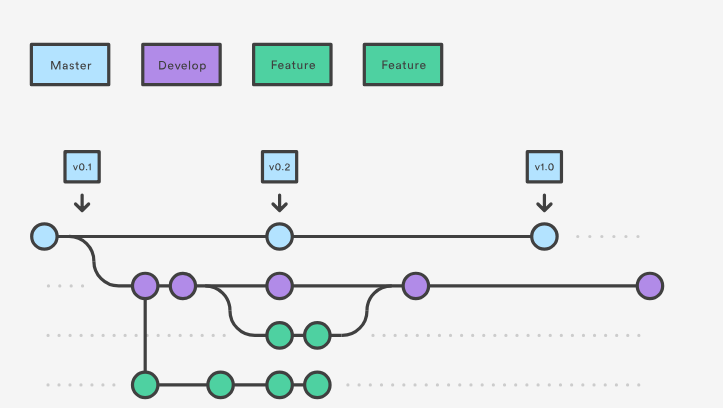
\includegraphics[width=\textwidth]{gfx/Git-Workflow.png}
	\captionsetup{justification=centering}
	\caption{Working of git workflow.}
	\label{fig:git-workflow}
\end{figure}

\subsection{Tags}
Tags are the process of assigning unique version numbers to unique states of the software packages. The tags are only created in the \textit{master} branch of the repository. For the ML4PdM project, we are going to follow the Semantic versioning tags for release packages. Semantic versioning is a standard convention for specifying compatibility using a three-part version number. We will follow the \textbf{Major.Minor.Patch} e.g.- v1.0.1, v1.0.0 format for our package release. The \textbf{Major} number is incremented when there are significant changes in functionality. The \textbf{Minor} number is incremented when only new features or major bug fixes have been added. The \textbf{Patch} number is incremented for minor changes and bug fixes.

\subsection{Commit Messages}
The content of the commit message outlining the change is just as important as the content of the change itself. For the ML4PdM project, we should use one of the below-listed commit constants in the subject line for the commit description.
\begin{enumerate}
	\item \textbf{[GEN]} - Use when code changes are related to general task like setup of document and etc.
	\item \textbf{[TFE]} - Use when code changes are related to Time Series Feature Extraction.
	\item \textbf{[HIE]} - Use when code changes are related to Health Index Estimation.
	\item \textbf{[RUL]} - Use when code changes are related to Remaining Useful Lifetime Estimation.
\end{enumerate}
While writing a commit message there are few important rules to keep in mind.
\begin{enumerate}
	\item Separate subject line from body with a blank line.
	\item Limit the subject line to 50 characters.
	\item Capitalize the subject line.
	\item Do not end the subject line with a period.
	\item Use the imperative mood in the subject line.
	\item Wrap the body at 72 characters.
	\item Can use the body to explain what and why vs how.
\end{enumerate}

\subsection{Merge}
The Merge command are designed to integrate changes from one branch into another branch. For ML4PdM project, We are using explicit merges (create new merge commit) strategy because it is simple, provide great traceability and context on the features being merged. The merge request should be reviewed by at least two people (Author and other team member) using GitLab approval feature in repository to maintain code quality. We are not going to squash and delete the source branch. Manual merge and rebase strictly not allowed in repository. The Figure \ref{fig:merge-request-template} show the merge request description template. Use the template, while requesting Merge Request (MR) to merge the proposed changes from one branch to another. In Added section, list or describe what are the new features added in proposed changes. In Changed section, list or describes the changes in the existing functionality. In Deprecated part, list or describe what are the feature will soon be removed. In Removed part, list or describe what features have been removed. In the Fixed part, list or describe what bugs fixes are.
\begin{figure}[ht]
	\centering
	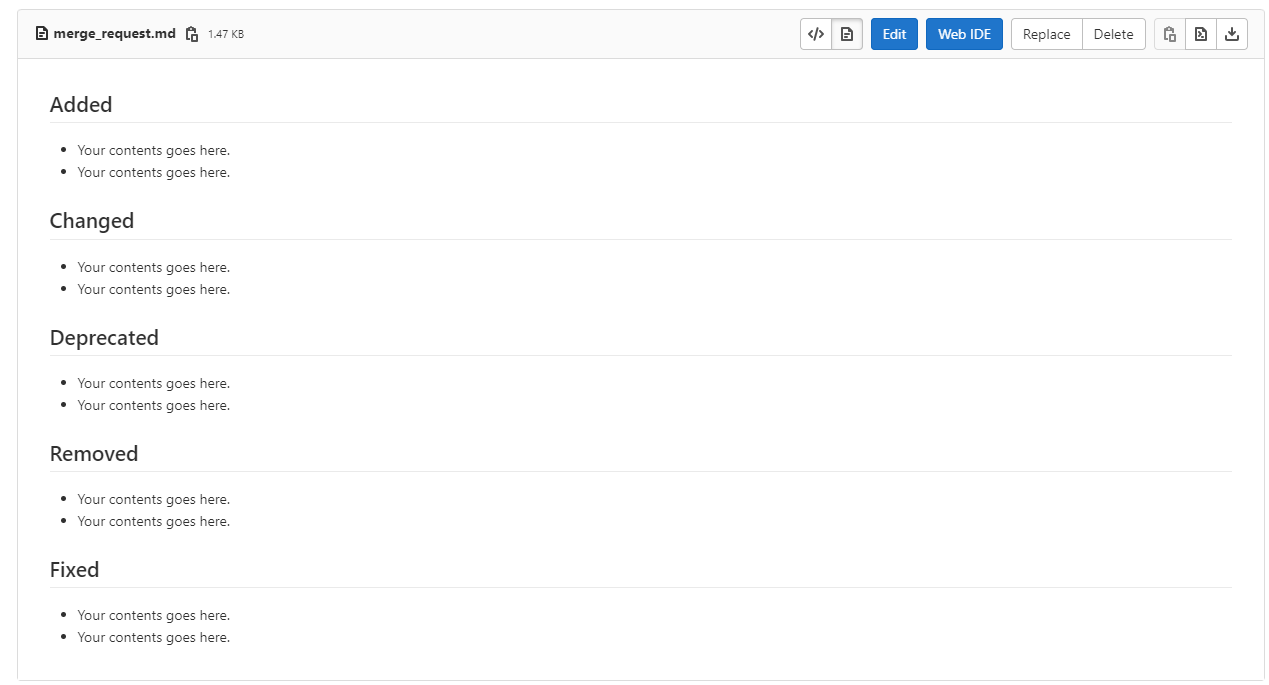
\includegraphics[width=\textwidth]{gfx/merge-request-template.PNG}
	\captionsetup{justification=centering}
	\caption{Structure of the Merge request template.}
	\label{fig:merge-request-template}
\end{figure}
               % INCLUDE: quality-assurance

% --------------------------
% Back matter
% --------------------------
% \appendix\cleardoublepage
% \input{content/chapter-appendix}       % INCLUDE: appendix
%
{%
    \setstretch{1.1}
    \renewcommand{\bibfont}{\normalfont\small}
    \setlength{\biblabelsep}{0pt}
    \setlength{\bibitemsep}{0.5\baselineskip plus 0.5\baselineskip}
    \printbibliography
    % [nottype=online]
    % \newrefcontext[labelprefix={@}]
    % \printbibliography[heading=subbibliography,title={Datasets},type=online]
}
\cleardoublepage
\listoffigures
\cleardoublepage
% \listoftables
% \cleardoublepage


% !TEX root = ../main.tex
%
\pagestyle{empty}
\hfill
\vfill
\pdfbookmark[0]{Colophon}{Colophon}
\section*{Colophon}

This thesis was typeset with \LaTeXe.
It uses the \textit{Clean Thesis} style developed by Ricardo Langner.
The design of the \textit{Clean Thesis} style is inspired by user guide documents from Apple Inc.

Download the \textit{Clean Thesis} style at \url{http://cleanthesis.der-ric.de/}.

% \cleardoublepage

% \input{content/declaration}
\clearpage
\newpage
\mbox{}

% **************************************************
% End of Document CONTENT
% **************************************************
\end{document}
